\section{Conventions}
\label{s:conv}
\thispagestyle{plain}

\subsection{Data Structure Notation Conventions}
\label{s:conv_language}

The intellectual content of the CGNS database is defined in terms of
C-like notation including typedefs and structures.  The database is made
up of entities, and each entity has a type associated with it.  Entities
include such things as the dimensionality of the grid, an array of grid
coordinates, or a zone which contains all the data associated with a
given region.  Entities are defined in terms of types, where a type can
be an integer or a collection of elements (a structure) or a hierarchy
of structures or other similar constructs.

The terminology ``instance of an entity'' is used to refer to an entity
that has been assigned a value or whose elements have been assigned
values.  The terminology ``specific instance of a structure'' is also used
in the following sections.  It is short for an instance of an entity
whose type is a structure.

Names of entities and types are constructed using conventions typical
of \textit{Mathematica}.\footnote{\textit{Mathematica 3.0}, Wolfram Research,
Inc., Champaign, IL (1996)}
Names or identifiers contain no spaces and capitalization is used to
distinguish individual words making up a name; names are case-sensitive.
The characters ``|.|'' and ``|/|'' should be avoided in names as these have
special meaning when referencing elements of a structure entity.

The following notational conventions are employed:

\begin{Ventryic}{\fort{Enumeration( )}}
\item [\fort{!}]
      comment to end of line
\item [\fort{\_t}]
      suffix used for naming a type
\item [\fort{;}]
      end of a definition, declaration, assignment or entity instance
\item [\fort{=}]
      assignment (takes on the value of)
\item [\fort{:=}]
      indicates a type definition (typedef)
\item [\fort{[ ]}]
      delimiters of an array
\item [\fort{\{ \}}]
      delimiters of a structure definition
\item [\fort{\{\{ \}\}}]
      delimiters of an instance of a structure entity
\item [\fort{< >}]
      delimiters of a structure parameter list
\item [\fort{int}]
      integer
\item [\fort{real}]
      floating-point number
\item [\fort{char}]
      character
\item [\fort{bit}]
      bit
\item [\fort{Enumeration( )}]
      indicates an enumeration type
\item [\fort{Data( )}]
      indicates an array of data, which may be multidimensional
\item [\fort{List( )}]
      indicates a list of entities
\item [\fort{Identifier( )}]
      indicates an entity identifier
\item [\fort{LogicalLink( )}]
      indicates a logical link
\item [\fort{/}]
      delimiter for element of a structure entity
\item [\fort{../}]
      delimiter for parent of a structure entity
\item [\fort{(r)}]
      designation for a required structure element
\item [\fort{(o)}]
      designation for an optional structure element
\item [\fort{(o/d)}]
      designation for an optional structure element with default if absent
\end{Ventryic} 

An enumeration type is a set of values identified by names; names of
values within a given enumeration declaration must be unique.  An
example of an enumeration type is the following:
\begin{alltt}
  Enumeration( Dog, Cat, Bird, Frog ) 
\end{alltt}
This defines an enumeration type which contains four values.  

|Data()| identifies an array of given dimensionality and size in each
dimension, whose elements are all of a given data type.
It is written as,
\begin{alltt}
  Data( DataType, Dimension, DimensionValues[] ) ;
\end{alltt}
|Dimension| is an integer, and |DimensionValues[]| is an array of integers
of size |Dimension|.
\texttt{Dimension} and \texttt{DimensionValues[]} specify the 
dimensionality of the array and its size in each dimension.
|DataType| specifies the data type of the array's elements; it may consist
of one of the following: |int|, |real|, |char| or |bit|.
For multidimensional arrays, FORTRAN indexing conventions are used.  
|Data()| is formulated to map directly onto the data section of an ADF node.

A typedef establishes a new type and defines it in terms of previously
defined types.
Types are identified by the suffix ``|_t|'', and the symbol ``|:=|'' is used
to establish a type definition (or typedef).
For example, the above enumeration example can be used in a typedef:
\begin{alltt}
  Pet\_t := Enumeration( Dog, Cat, Bird, Frog ) ;
\end{alltt}
This defines a new type |Pet_t|, which can then be used to declare a new
entity, such as,
\begin{alltt}
  Pet\_t MyFavoritePet ;
\end{alltt}
By the above typedef and declaration, |MyFavoritePet| is an entity of type
|Pet_t| and can have the values |Dog|, |Cat|, |Bird| or |Frog|.
A specific instance of |MyFavoritePet| is setting it equal to one of these
values (e.g., |MyFavoritePet| |=| |Bird|).

A structure is a type that can contain any number of elements, including
elements that are also structures.
An example of a structure type definition is:
\begin{alltt}
  Sample\_t :=
    \{
    int Dimension ;                                                         (r)

    real[4] Vector ;                                                        (o)

    Pet\_t ObnoxiousPet ;                                                    (o)
    \} ;
\end{alltt}
where |Sample_t| is the type of the structure.
This structure contains three elements, |Dimension|, |Vector| and
|ObnoxiousPet|, whose types are |int|, |real[4]| and |Pet_t|, respectively.
The type |int| specifies an integer, and |real[4]| specifies an array of
reals that is one-dimensional with a length of four.
The ``|(r)|'' and ``|(o)|'' notation in the right margin is explained below.
Given the definition of |Sample_t|, entities of this type can then be
declared (e.g., |Sample_t| |Sample1;|).
An example of an instance of a structure entity is given by,
\begin{alltt}
  Sample\_t Sample1 = 
    \{\{
    Dimension = 3 ;
    Vector = [1.0, 3.45, 2.1, 5.4] ;
    ObnoxiousPet = Dog ;
    \}\} ;
\end{alltt}
Note the different functions played by single braces ``|{|'' and double
braces ``|{{|''.
The first is used to delimit the definition of a structure type; the
second is used to delimit a specific instance of a structure entity.

Some structure type definitions contain arbitrarily long lists of other
structures or types.
These lists will be identified by the notation,
\begin{alltt}
  List( Sample\_t Sample1 ... SampleN ) ;
\end{alltt}
where |Sample1 ... SampleN| is the list of structure names or
identifiers, each of which has the type |Sample_t|.
Within each list, the individual structure names are user-defined.

In the CGNS database it is sometimes necessary to reference the name or
identifier of a structure entity.  References to entities are denoted by
|Identifier()|, whose single argument is a structure type.  For example,
\begin{alltt}
  Identifier(Sample\_t) SampleName ;
\end{alltt}
declares an entity, |SampleName|, whose value is the identifier of
a structure entity of type |Sample_t|.
Given this declaration, |SampleName| could be assigned the value
|Sample1| (i.e., |SampleName| = |Sample1|).

It is sometimes convenient to directly identify an element of a specific
structure entity.  It is also convenient to indicate that two entities
with different names are actually the same entity.  We borrow UNIX
conventions to indicate both these features, and make the analogy
that a structure entity is a UNIX directory and its elements are UNIX
files.  An element of an entity is designated by ``|/|''; an example is
|Sample1/Vector|).  The structure entity that a given element belongs
to is designated ``|../|'' A UNIX-like logical link that specifies
the sameness of two apparently different entities is identified by
|LogicalLink()|; it has one argument.  An example of a logical link is
as follows:  Suppose a specific instance of a structure entity contains
two elements that are of type |Sample_t|; call them |SampleA| and
|SampleB|.  The statement that |SampleB| is actually the same entity as
|SampleA| is,
\begin{alltt}
  SampleB = LogicalLink(../SampleA) ;
\end{alltt}
The argument of |LogicalLink()| is the UNIX-like ``path name'' of the
entity with which the link is made.
In this document, |LogicalLink()| and the direct specification of a
structure element via ``|/|'' and ``|../|'' are actually seldom used.
These language elements are never used in the actual definition of a
structure type.

Structure type definitions include three additional syntactic/semantic
notions.
These are parameterized structures, structure-related functions, and the
identification of required and optional fields within a structure.

As previously stated, one of our design objectives is to minimize
duplication of information within the CGNS database.  To meet this
objective, information is often stored in only one location of the
hierarchy; however, that information is typically used in other parts
of the hierarchy.  A consequence of this is that it may not be possible
to decipher all the information associated with a given entity in the
hierarchy without knowledge of data contained in higher level entities.
For example, the grid size of a zone is stored in one location (in
|Zone_t|, see \autoref{s:Zone}), but is needed in many substructures to
define the size of grid and solution-data arrays.

This organization of information must be reflected in the language
used to describe the database.  First, parameterized structures are
introduced to formalize the notion that information must be passed down
the hierarchy.  A given structure type is defined in terms of a list
of parameters that precisely specify what information must be obtained
from the structure's parent.  These structure-defining parameters
play a similar role to subroutine parameters in C or FORTRAN and are
used to define fields within the structure; they are also passed onto
substructures.  Parameterized structures are also loosely tied to
templates in C++.

Parameterized structures are identified by the delimiters |< >|
enclosing the list of parameters.
Each structure parameter in a structure-type definition consists of a
type and an identifier.
Examples of parameterized structure type definitions are:
\begin{alltt}
  NewSample\_t< int Dimension, int Fred > :=
    \{
    int[Dimension] Vector ;                                                 (o)

    Pet\_t ObnoxiousPet ;                                                    (o)

    Stuff\_t<Fred> Thingy ;                                                  (o)
    \} ;

  Stuff\_t< int George > :=
    \{
    real[George] IrrelevantStuff ;                                          (r)
    \} ;
\end{alltt}
|NewSample_t| and |Stuff_t| are parameterized structure types.  |Dimension|
and |Fred| are the structure parameters of |NewSample_t|.  |George| is the
structure parameter of |Stuff_t|.  All structure parameters in this example
are of type |int|.  |Thingy| is a structure entity of type |Stuff_t|; it uses
the parameter |Fred| to complete its declaration.  Note the use of |George|
and |Fred| in the above example.  |George| is a parameter in the definition
of |Stuff_t|; |Fred| is an argument in the declaration of an entity of type
|Stuff_t|.  This mimics the use of parameters in function definitions in C.

A second language feature required to cope with the cascade of information
within the hierarchy is structure-related functions.  For example, the size
of an array within a given structure may be a function of one or more of the
structure-defining parameters, or the array size may be a function of an
optional field within the structure.  No new syntax is provided to
incorporate structure-related functions; they are instead described in terms
of their return values, dependencies, and functionality.

An additional notation used in structure typedefs is that each element or
field within a structure definition is identified as required, optional, or
optional with a default if absent; these are designated by ``|(r)|'', ``|(o)|'',
and ``|(o/d)|'', respectively, in the right margin of the structure
definition.  These designations are included to assist in implementation of
the data structures into an actual database and can be used to guide mapping
of data as well as error checking.  ``Required'' fields are those essential to
the interpretation of the information contained within the data structure.
``Optional'' fields are those that are not necessary but potentially useful,
such as documentation.  ``Defaulted-optional'' fields are those that take on a
known default if absent from the database.

In the example of |Sample_t| above, only the element |Dimension| is
required.  Both elements |Vector| and |ObnoxiousPet| are optional.  This
means that in any specific instance of the structure, only |Dimension|
must be present.  An alternative instance of the entity |Sample1| shown
above is the following:
\begin{alltt}
  Sample\_t Sample1 = 
    \{\{
    Dimension = 4 ;
    \}\} ;
\end{alltt}

None of the entities and types defined in the above examples are actually
used in the definition of the SIDS.

As a final note, the reader should be aware that the SIDS is a 
conceptual description of the form of the data.
The actual location of data in the file is determined by the file
mapping, defined by the appropriate \textit{File Mapping Manual}.

\subsection{Structured Grid Notation and Indexing Conventions} 
\label{s:structgrid}

A \emph{grid} is defined by its vertices.  In a 3-D structured grid,
the volume is the ensemble of cells, where each cell is the hexahedron
region defined by eight nearest neighbor vertices.  Each cell is bounded
by six faces, where each face is the quadrilateral made up of four
vertices.  An edge links two nearest-neighbor vertices; a face is
bounded by four edges.

In a 2-D structured grid, the notation is more ambiguous.  Typically,
the quadrilateral area composed of four nearest-neighbor vertices
is referred to as a cell.  The sides of each cell, the line linking
two vertices, is either a face or an edge.  In a 1-D grid, the line
connecting two vertices is a cell.

A \emph{structured multizone grid} is composed of multiple regions
called \emph{zones}, where each zone includes all the vertices, cells,
faces, and edges that constitute the grid in that region.

Indices describing a 3-D grid are ordered $(i,j,k)$;
$(i,j)$ is used for 2-D and $(i)$ for 1-D.

Cell centers, face centers, and edge centers are indexed by the minimum
$i$, $j$, and $k$ indices of the connecting vertices.
For example, a 2-D cell center (or face center on a 3-D grid) would have
the following convention:

\begin{center}
\begin{picture}(4,1.2)
% \put(0,0){ \framebox(2,1){} }
% \put(2,0){ \framebox(2,1){} }

 \multiput(0,0)(0,1){2}{ \line(1,0){4} }
 \multiput(0,0)(2,0){3}{ \line(0,1){1} }
 \multiput(0,0)(2,0){3}{ \makebox(0,0){$\bullet$} }
 \multiput(0,1)(2,0){3}{ \makebox(0,0){$\bullet$} }

 \put(1,0.5){ \makebox(0,0){\small $(i,j)$} }
 \put(3,0.5){ \makebox(0,0){\small $(i+1,j)$} }

 \put(0,-0.05){ \makebox(0,0)[t]{\small $(i,j)$} }
 \put(2,-0.05){ \makebox(0,0)[t]{\small $(i+1,j)$} }
 \put(4,-0.05){ \makebox(0,0)[t]{\small $(i+2,j)$} }
 \put(0, 1.08){ \makebox(0,0)[b]{\small $(i,j+1)$} }
 \put(2, 1.08){ \makebox(0,0)[b]{\small $(i+1,j+1)$} }
 \put(4, 1.08){ \makebox(0,0)[b]{\small $(i+2,j+1)$} }
\end{picture}
\end{center}

\noindent
In addition, the default beginning vertex for the grid in a given
zone is $(1,1,1)$; this means the default beginning cell center of the
grid in that zone is also $(1,1,1)$.

A zone may contain grid-coordinate or flow-solution data defined at a
set of points outside the zone itself.
These are referred to as ``rind'' or ghost points and may be associated
with fictitious vertices or cell centers.
They are distinguished from the vertices and cells making up the grid
within the zone (including its boundary vertices), which are referred to
as ``core'' points.
The following is a 2-D zone with a single row of rind vertices at the
minimum and maximum $i$-faces.
The grid size (i.e., the number of core vertices in each direction) is
$5\cross4$. Core vertices are designated by ``$\bullet$'', and rind
vertices by ``$\times$''.
Default indexing is also shown for the vertices.

\begin{center}
\begin{picture}(4,1)(0,-0.25)
% \put(0,0){ \framebox(2,1){} }
% \put(2,0){ \framebox(2,1){} }

\multiput(0,0)(0,0.25){4}{ \line(1,0){4.0} }
\multiput(0,0)(1,0){5}{ \line(0,1){0.75} }

\multiput(0,0.00)(1,0){5}{ \makebox(0,0){$\bullet$} }
\multiput(0,0.25)(1,0){5}{ \makebox(0,0){$\bullet$} }
\multiput(0,0.50)(1,0){5}{ \makebox(0,0){$\bullet$} }
\multiput(0,0.75)(1,0){5}{ \makebox(0,0){$\bullet$} }

\multiput(-1,0)(0,0.25){3}{ \dashbox{0.05}(1.0,0.25){} }
\multiput(-1,0)(0,0.25){4}{ \makebox(0,0){$\times$} }

\multiput(4,0)(0,0.25){3}{ \dashbox{0.05}(1.0,0.25){} }
\multiput(5,0)(0,0.25){4}{ \makebox(0,0){$\times$} }

\put(-1,-0.05){ \makebox(0,0)[t]{$(0,1)$} }
\put( 0,-0.05){ \makebox(0,0)[t]{$(1,1)$} }
\put( 4,-0.05){ \makebox(0,0)[t]{$(5,1)$} }
\put( 5,-0.05){ \makebox(0,0)[t]{$(6,1)$} }

\put( 4,0.83){ \makebox(0,0)[b]{$(5,4)$} }
\end{picture}
\end{center}

For a zone, the minimum faces in each coordinate direction are denoted
$i$-min, $j$-min and $k$-min; the maximum faces are denoted $i$-max,
$j$-max and $k$-max.
These are the minimum and maximum core faces.
For example, $i$-min is the face or grid plane whose core vertices
have minimum $i$ index (which if using default indexing is 1).

\subsection{Unstructured Grid Element Numbering Conventions} 
\label{s:unstructgrid}

The major difference in the way structured and unstructured grids are
recorded is the element definition.
In a structured grid, the elements can always be recomputed easily
using the computational coordinates, and therefore they are usually
not written in the data file.
For an unstructured grid, the element connectivity cannot be easily
built, so this additional information is generally added to the data file.
The element information typically includes the element type or shape,
and the list of nodes for each element.

In an unstructured zone, the nodes are ordered from 1 to $N$, where $N$
is the number of nodes in the zone.
An element is defined as a group of one or more nodes, where each node
is represented by its index.
The elements are indexed from 1 to $M$ within a zone, where $M$
is the total number of elements defined for the zone.

CGNS supports eight element shapes --- points, lines, triangles,
quadrangles, tetrahedra, pentahedra, pyramids, and hexahedra.
Elements describing a volume are referred to as 3-D elements.
Those defining a surface are 2-D elements.
Line and point elements are called 1-D and 0-D elements, respectively.

In a 3-D unstructured mesh, the cells are defined using 3-D elements,
while the boundary patches may be described using 2-D elements.
The complete element definition may include more than just the cells.

Each element shape may have a different number of nodes, depending on
whether linear, quadratic, or cubic interpolation is used.
Therefore the name of each type of element is composed of two parts;
the first part identifies the element shape, and the second part the
number of nodes.
\autoref{t:elementtypes} summarizes the element types supported in CGNS.

\begin{table}[htbp]
\centering
\caption[Element Types in CGNS]{\textbf{Element Types in CGNS}}
\label{t:elementtypes}
\begin{tabular}{c >{\quad}l >{\quad}l >{\quad}l >{\quad}l}
\\ \hline\hline \\*[-2ex]
\bold{Dimensionality} &                        & \bold{Linear}        & \bold{Quadratic}     & \bold{Cubic}\\
\bold{of the Element} & \spantwo{\bold{Shape}} & \bold{Interpolation} & \bold{Interpolation} & \bold{Interpolation}
\\*[1ex] \hline\hline \\*[-2ex]
0-D & Point       & \fort{NODE}     & \fort{NODE}                 & \fort{NODE} \\
1-D & Line        & \fort{BAR\_2}   & \fort{BAR\_3}               & \fort{BAR\_4} \\
2-D & Triangle    & \fort{TRI\_3}   & \fort{TRI\_6}               & \fort{TRI\_9, TRI\_10} \\
    & Quadrangle  & \fort{QUAD\_4}  & \fort{QUAD\_8,}             & \fort{QUAD\_12,} \\
    &             &                 & \fort{QUAD\_9}              & \fort{QUAD\_16} \\
3-D & Tetrahedron & \fort{TETRA\_4} & \fort{TETRA\_10}            & \fort{TETRA\_16, TETRA\_20} \\
    & Pyramid     & \fort{PYRA\_5}  & \fort{PYRA\_13,}            & \fort{PYRA\_21, PYRA\_29,} \\
    &             &                 & \fort{PYRA\_14}             & \fort{PYRA\_30} \\
    & Pentahedron & \fort{PENTA\_6} & \fort{PENTA\_15,}           & \fort{PENTA\_24, PENTA\_38,} \\
    &             &                 & \fort{PENTA\_18}            & \fort{PENTA\_40} \\
    & Hexahedron  & \fort{HEXA\_8}  & \fort{HEXA\_20,}            & \fort{HEXA\_32, HEXA\_56,} \\
    &             &                 & \fort{HEXA\_27}             & \fort{HEXA\_64}
\\*[1ex] \hline\hline
\end{tabular}
\end{table}

General polyhedral elements can be recorded using the CGNS
generic element types \fort{NGON\_n} and \fort{NFACE\_n}.
See \autoref{s:Elements} for more detail.

The ordering of the nodes within an element is important.
Since the nodes in each element type could be ordered in multiple ways,
it is necessary to define numbering conventions.
The following sections describe the element numbering conventions
used in CGNS.

Like a structured zone, an unstructured zone may contain
grid-coordinates or flow-solution data at points outside of the zone
itself, through the use of ghost or ``rind'' points and elements.
However, unlike for structured zones, rind data for unstructured zones
cannot be defined implicitly (i.e., via indexing conventions alone).
In other words, when using rind with unstructured zones, the rind grid
points and their element connectivity information should always be
given.

\setlength{\tmplength}{0.25\linewidth-1.25in}

\subsubsection{1-D (Line) Elements}

1-D elements represent geometrically a line (or bar).
The linear form, \fort{BAR\_2}, is composed of two nodes at each
extremity of the line.
The quadratic form, \fort{BAR\_3}, has an additional node located at
the middle of the line.
The cubic form of the line, \fort{BAR\_4}, contains two nodes
interior to the endpoints.

\underbar{Linear and Quadratic Elements:}

\begin{minipage}[t]{0.5\linewidth}
   \vspace{0pt}
   \centering
   \hspace*{\tmplength}\fort{BAR\_2}\hfill\mbox{} \\[\baselineskip]
   \begin{picture}(2.0,0.0)
      \drawline(0.0,0.0)(2.0,0.0)
      \put( 0.00, 0.00){\circle*{0.1}}
      \put(-0.10, 0.00){\makebox(0,0)[r]{1}}
      \put( 2.00, 0.00){\circle*{0.1}}
      \put( 2.10, 0.00){\makebox(0,0)[l]{2}}
   \end{picture}
\end{minipage}%
\begin{minipage}[t]{0.5\linewidth}
   \vspace{0pt}
   \centering
   \hspace*{\tmplength}\fort{BAR\_3}\hfill\mbox{} \\[\baselineskip]
   \begin{picture}(2.0,0.1)
      \drawline(0.0,0.0)(2.0,0.0)
      \put( 0.00, 0.00){\circle*{0.1}}
      \put(-0.10, 0.00){\makebox(0,0)[r]{1}}
      \put( 2.00, 0.00){\circle*{0.1}}
      \put( 2.10, 0.00){\makebox(0,0)[l]{2}}
      \put( 1.00, 0.00){\color{red}\circle*{0.1}}
      \put( 0.95,-0.05){\color{red}\makebox(0,0)[rt]{3}}
   \end{picture}
\end{minipage}

\bigskip

\begin{tabular}{@{}>{\ttfamily}c >{\ttfamily}c >{\ttfamily\color{red}}c}
   \multicolumn{3}{@{}l}{\uline{\textit{Edge Definition}}} \\[6pt]
   \uline{\textnormal{Oriented edge}} & \uline{\textnormal{Corner nodes}} & \uline{\textnormal{Mid-node}} \\[3pt]
   E1 & N1,N2 & N3
\end{tabular}

\underbar{Cubic Elements:}

BAR\_4
\begin{figure}[!htb]
%   \centering
   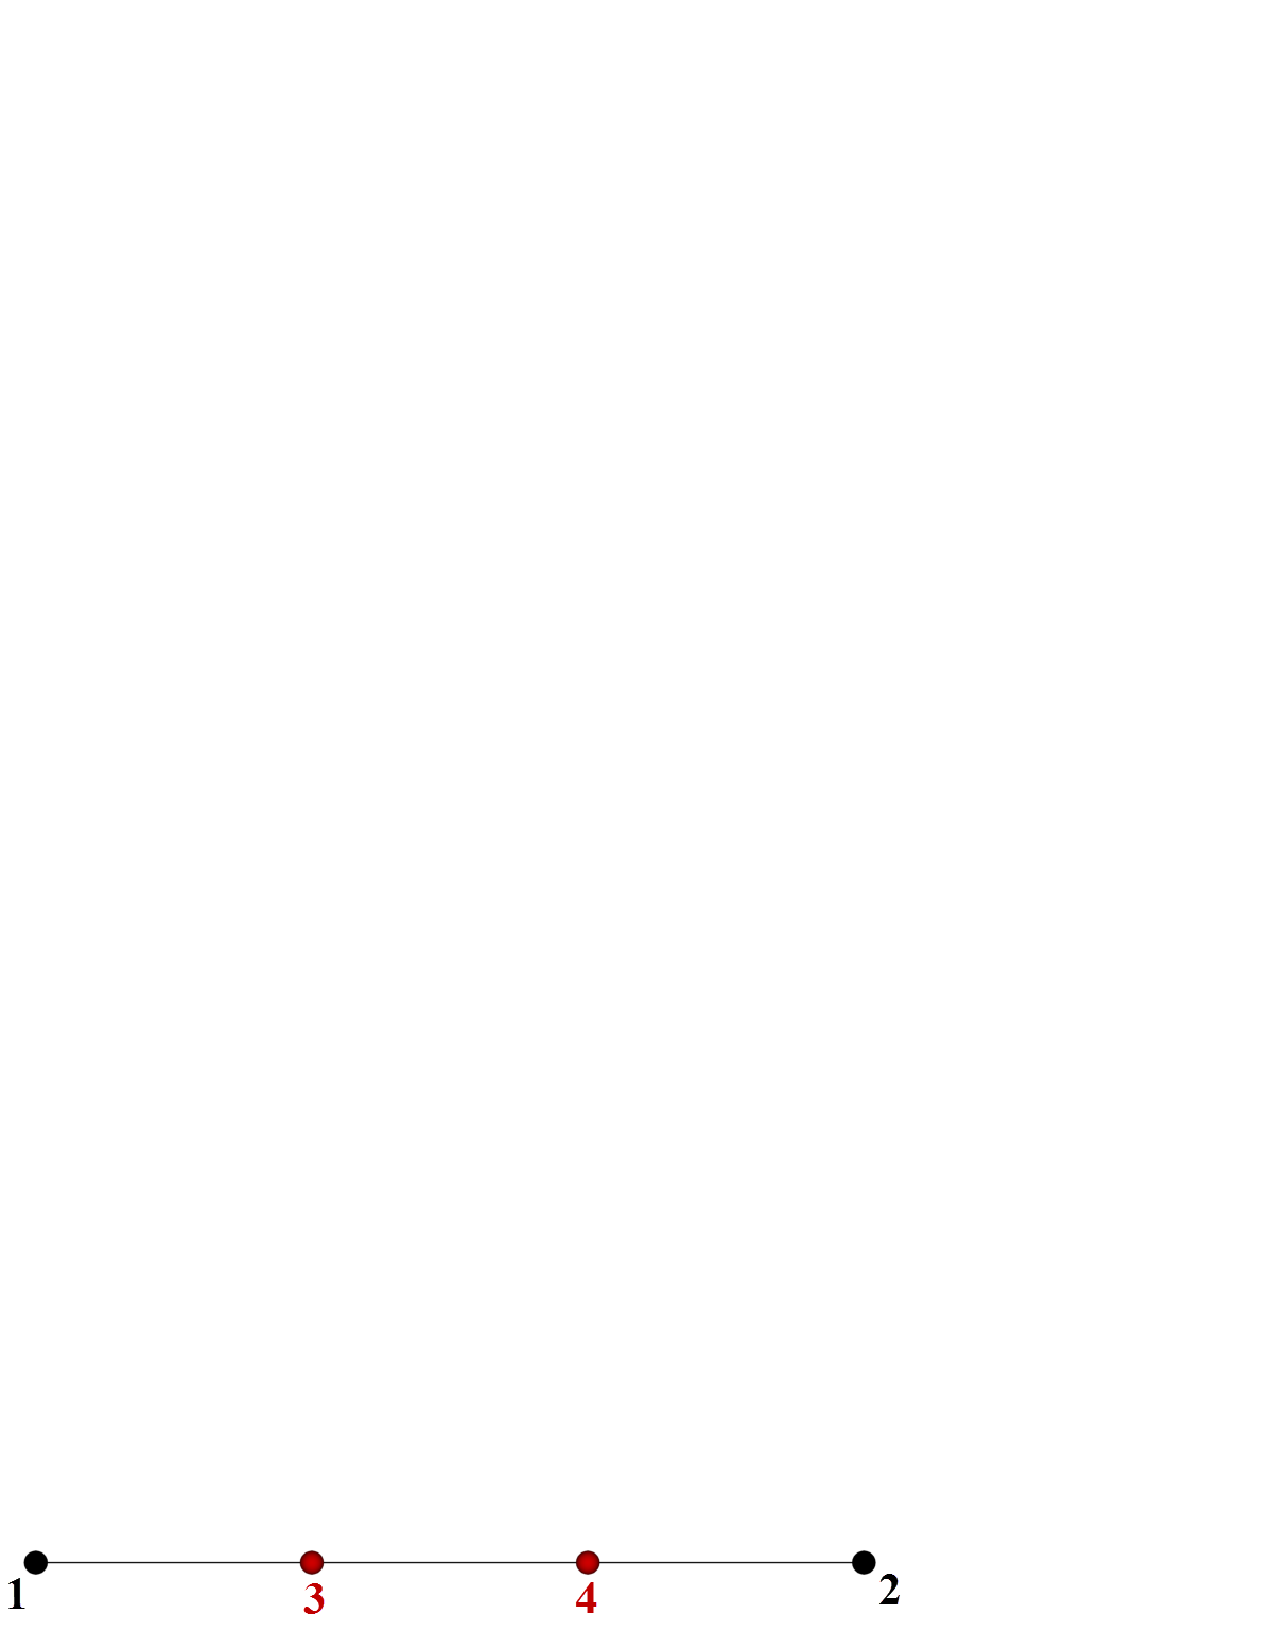
\includegraphics[width=3in]{conv.figs/TecplotFiles_Cubic_Element/All_Figures/bar_p3}
\end{figure}

\begin{tabular}{@{}>{\ttfamily}c >{\ttfamily}c >{\ttfamily\color{red}}c}
   \multicolumn{3}{@{}l}{\uline{\textit{Edge Definition}}} \\[6pt]
   \uline{\textnormal{Oriented edge}} & \uline{\textnormal{Corner nodes}} & \uline{\textnormal{Mid-nodes}} \\[3pt]
   E1 & N1,N2 & N3,N4
\end{tabular}

\subsubsection{2-D (Surface) Elements}
\label{s:unstructgrid_2d}

2-D elements represent a surface in either 2-D or 3-D space.
Note that in physical space, the surface need not be planar, but
may be curved.
In a 2-D mesh the elements represent the cells themselves; in a 3-D
mesh they represent faces.
CGNS supports two shapes of 2-D elements --- triangles and quadrangles.

The normal vector of a 2-D element is computed using the cross product
of a vector from the first to second node, with a vector from the first
to third node.
The direction of the normal is such that the three
vectors (i.e., $(\overrightarrow{N2} - \overrightarrow{N1})$, 
$(\overrightarrow{N3} - \overrightarrow{N1})$, and $\overrightarrow{N}$)
form a right-handed triad.
$$
\overrightarrow{N} = (\overrightarrow{N2} - \overrightarrow{N1}) \times
                     (\overrightarrow{N3} - \overrightarrow{N1})
$$
In a 2-D mesh, all elements must be oriented the same way; i.e., all
normals must point toward the same side of the mesh.

\paragraph{Triangular Elements}
Four types of triangular elements are supported in CGNS, \fort{TRI\_3},
\fort{TRI\_6}, \fort{TRI\_9}, and \fort{TRI\_10}.
\fort{TRI\_3} elements are composed of three nodes located at the
three geometric corners of the triangle.
\fort{TRI\_6} elements have three additional nodes located at the
middles of the three edges.
The cubic forms of triangular elements, \fort{TRI\_9} and \fort{TRI\_10}
contain two interior nodes along each edge, and an interior face node
in the case of \fort{TRI\_10}.

\underbar{Linear and Quadratic Elements:}

\begin{minipage}[t]{0.5\linewidth}
   \vspace{0pt}
   \centering
   \hspace*{\tmplength}\fort{TRI\_3}\hfill\mbox{} \\[\baselineskip]
   \begin{picture}(2.0,0.75)
      \drawline(0.0,0.75)(2.0,0.75)(1.0,0.0)(0.0,0.75)
      \put( 1.00, 0.00){\circle*{0.1}}
      \put( 0.95,-0.05){\makebox(0,0)[rt]{1}}
      \put( 2.00, 0.75){\circle*{0.1}}
      \put( 2.10, 0.75){\makebox(0,0)[l]{2}}
      \put( 0.00, 0.75){\circle*{0.1}}
      \put(-0.10, 0.75){\makebox(0,0)[r]{3}}
      \put(1.00,0.50){\vector(0,1){0.5}}
      \put(1.10,1.00){\makebox(0,0)[l]{$\overrightarrow{N}$}}
   \end{picture}
\end{minipage}%
\begin{minipage}[t]{0.5\linewidth}
   \vspace{0pt}
   \centering
   \hspace*{\tmplength}\fort{TRI\_6}\hfill\mbox{} \\[\baselineskip]
   \begin{picture}(2.0,0.75)
      \drawline(0.0,0.75)(2.0,0.75)(1.0,0.0)(0.0,0.75)
      \put( 1.00, 0.00){\circle*{0.1}}
      \put( 0.95,-0.05){\makebox(0,0)[rt]{1}}
      \put( 2.00, 0.75){\circle*{0.1}}
      \put( 2.10, 0.75){\makebox(0,0)[l]{2}}
      \put( 0.00, 0.75){\circle*{0.1}}
      \put(-0.10, 0.75){\makebox(0,0)[r]{3}}
      {\color{red}
       \dashline[25]{0.025}(0.5,0.375)(1.5,0.375)(1.0,0.75)(0.5,0.375)
      }
      \put( 1.50, 0.375){\color{red}\circle*{0.1}}
      \put( 1.55, 0.325){\color{red}\makebox(0,0)[lt]{4}}
      \put( 1.00, 0.75 ){\color{red}\circle*{0.1}}
      \put( 0.95, 0.80 ){\color{red}\makebox(0,0)[rb]{5}}
      \put( 0.50, 0.375){\color{red}\circle*{0.1}}
      \put( 0.45, 0.325){\color{red}\makebox(0,0)[rt]{6}}
   \end{picture}
\end{minipage}

\vspace{1.5\baselineskip}

\begin{minipage}[t]{0.35\linewidth}
   \vspace{0pt}
   \begin{tabular}{@{}>{\ttfamily}l >{\ttfamily}l >{\ttfamily\color{red}}l}
      \multicolumn{3}{@{}l}{\uline{\textit{Edge Definition}}} \\[6pt]
      \textnormal{Oriented}      & \textnormal{Corner}	   & \textnormal{Mid-} \\
      \uline{\textnormal{edges}} & \uline{\textnormal{nodes}} & \uline{\textnormal{node}} \\[3pt]
      E1  & N1,N2 & N4 \\
      E2  & N2,N3 & N5 \\
      E3  & N3,N1 & N6
   \end{tabular}
\end{minipage}%
\begin{minipage}[t]{0.65\linewidth}
   \vspace{0pt}
   \begin{tabular}{@{}>{\ttfamily}c >{\ttfamily}l >{\ttfamily\color{red}}l >{\ttfamily}l}
      \multicolumn{4}{@{}l}{\uline{\textit{Face Definition}}} \\[6pt]
      \uline{\textnormal{Face}} & \uline{\textnormal{Corner nodes}} & \uline{\textnormal{Mid-edge nodes}} & \uline{\textnormal{Oriented edges}} \\[3pt]
      F1 & N1,N2,N3 & N4,N5,N6  & E1,E2,E3
   \end{tabular}
\end{minipage}

\underbar{Cubic Elements:}

TRI\_9~~~~~~~~~~~~~~~~~~~~~~~~~~~~~~~~~~~~~~~~~~~~~~~~~~~~TRI\_10
\begin{figure}[!htb]
%   \centering
   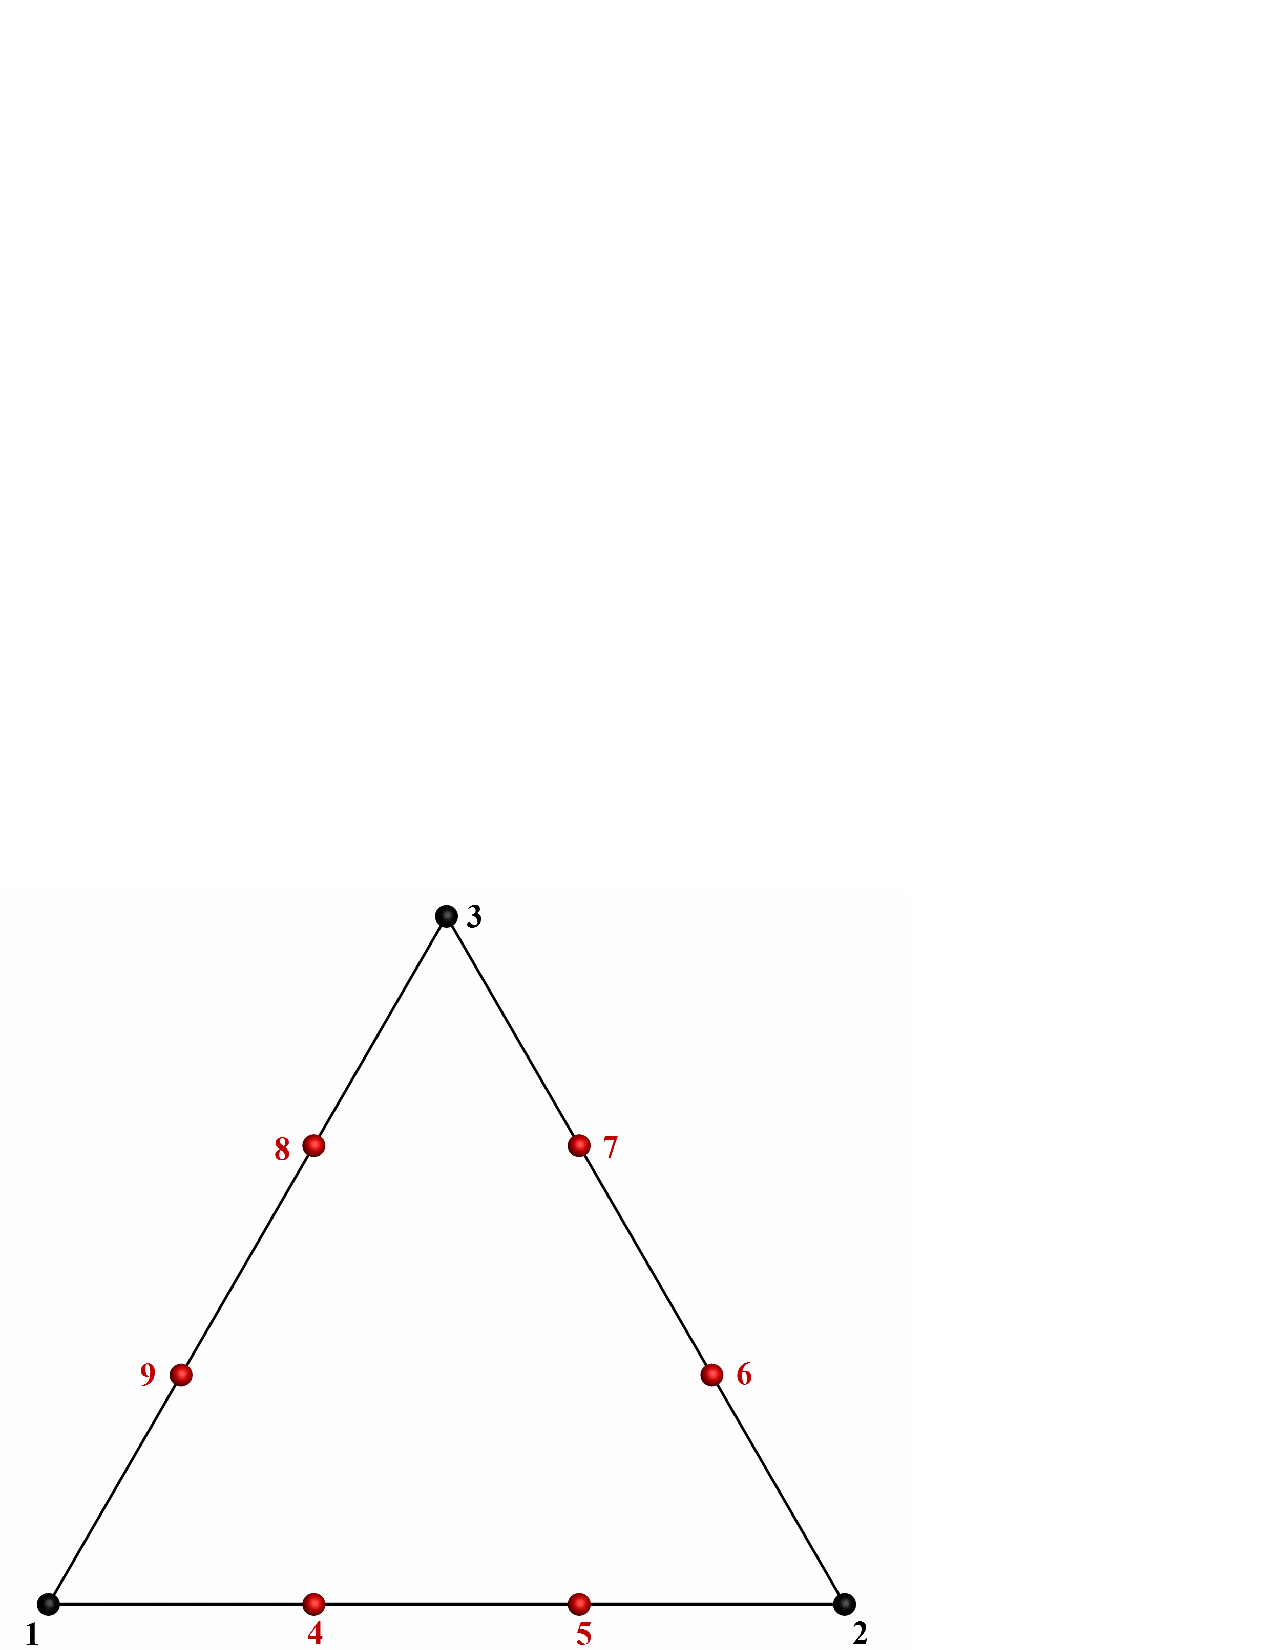
\includegraphics[width=2.5in]{conv.figs/TecplotFiles_Cubic_Element/All_Figures/Tri_9}
   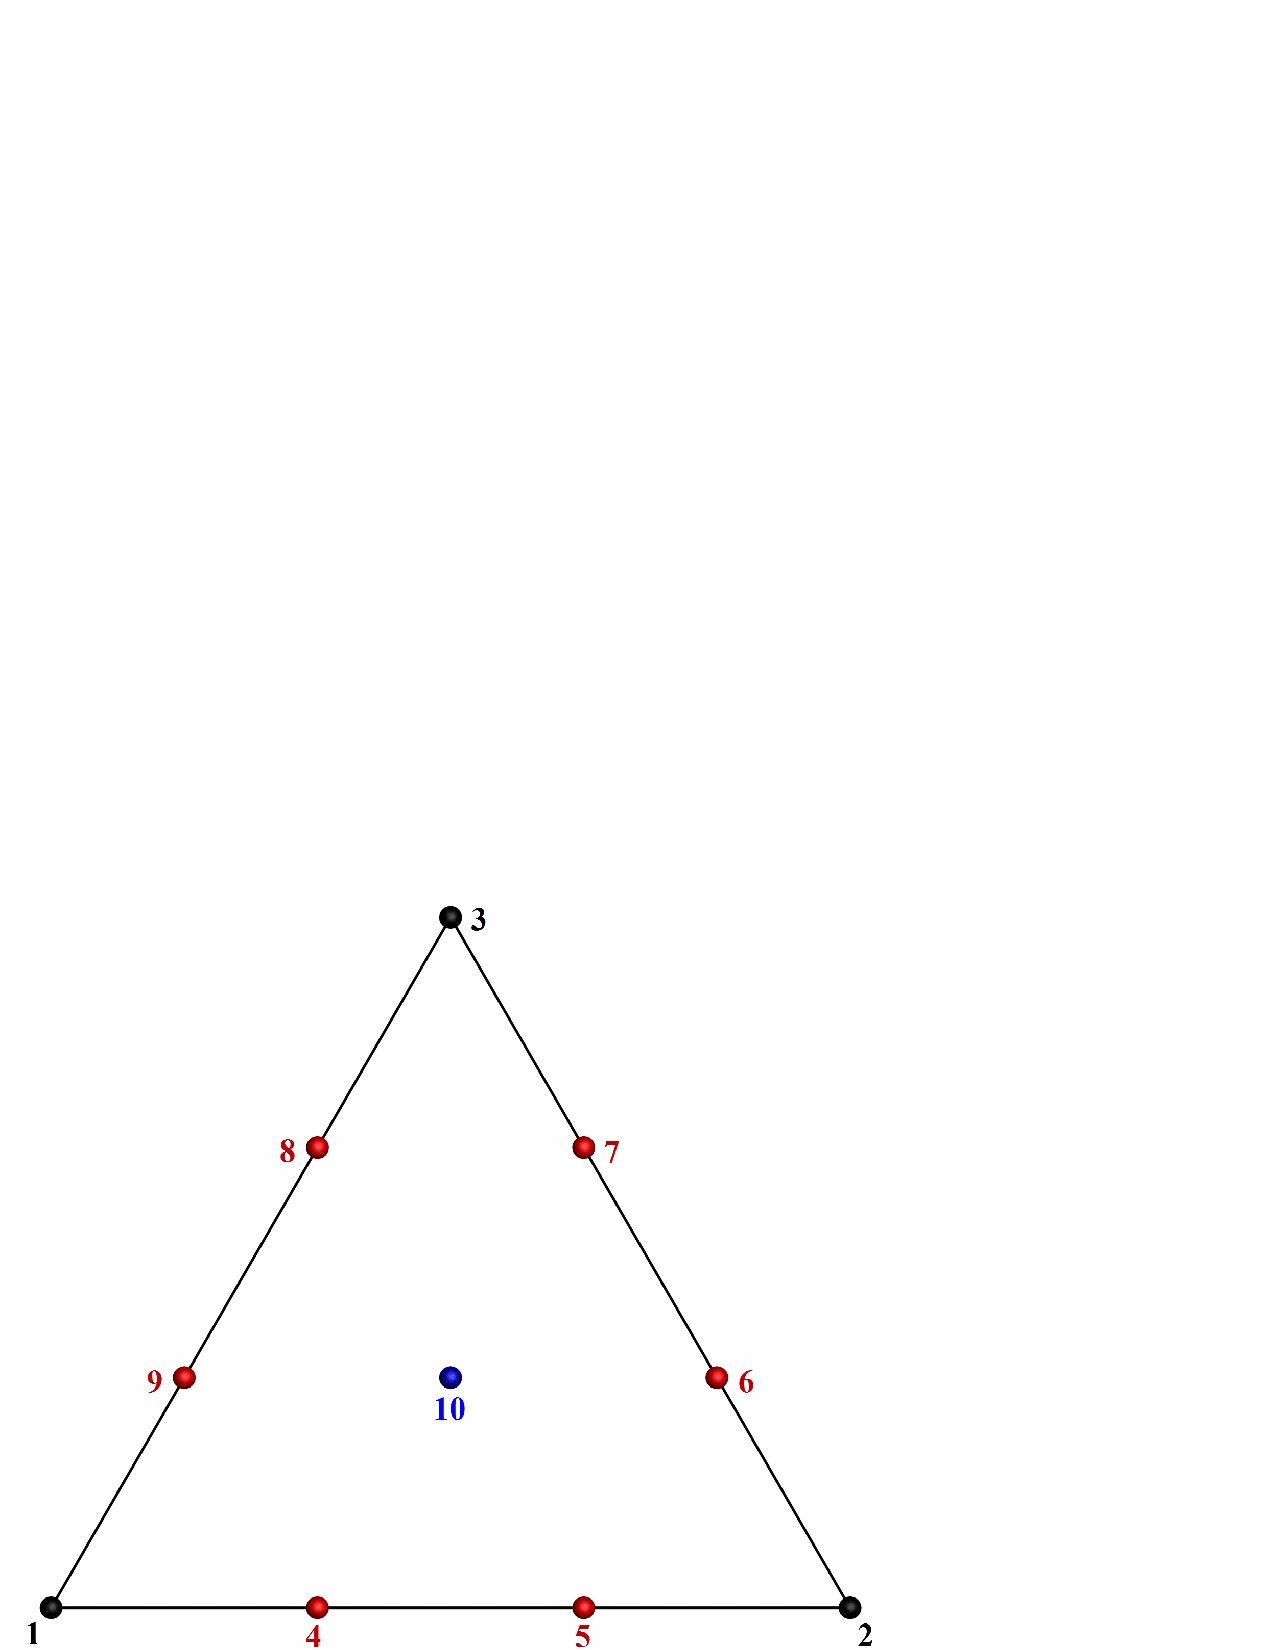
\includegraphics[width=2.5in]{conv.figs/TecplotFiles_Cubic_Element/All_Figures/Tri_10}
\end{figure}

\vspace{1.5\baselineskip}

\begin{minipage}[t]{0.35\linewidth}
   \vspace{0pt}
   \begin{tabular}{@{}>{\ttfamily}l >{\ttfamily}l >{\ttfamily\color{red}}l}
      \multicolumn{3}{@{}l}{\uline{\textit{Edge Definition}}} \\[6pt]
      \textnormal{Oriented}      & \textnormal{Corner}     & \textnormal{Mid-} \\
      \uline{\textnormal{edges}} & \uline{\textnormal{nodes}} & \uline{\textnormal{node}} \\[3pt]
      E1  & N1,N2 & N4,N5 \\
      E2  & N2,N3 & N6,N7 \\
      E3  & N3,N1 & N8,N9
   \end{tabular}
\end{minipage}%
\begin{minipage}[t]{0.65\linewidth}
   \vspace{0pt}
   \begin{tabular}{@{}>{\ttfamily}c >{\ttfamily}l >{\ttfamily\color{red}}l >{\ttfamily\color{blue}}l >{\ttfamily}l}
      \multicolumn{5}{@{}l}{\uline{\textit{Face Definition}}} \\[6pt]
      \textnormal{Face} & \textnormal{Corner} & \textnormal{Mid-edge} & \textnormal{Mid-face} & \textnormal{Oriented} \\
      \uline{\textnormal{}} & \uline{\textnormal{nodes}} & \uline{\textnormal{nodes}} & \uline{\textnormal{node}} & \uline{\textnormal{edges}} \\[3pt]
      F1 & N1,N2,N3 & N4,N5,N6,N7,N8,N9  & N10  & E1,E2,E3
   \end{tabular}
\end{minipage}

\bigskip

\uline{\textit{Notes}}%
\begin{Ventryi}{\fort{N1,\ldots,N27}}
   \item [\fort{N1,\ldots,N10}]
         Grid point identification number.
         Integer $\ge 0$ or blank, and no two values may be the same.
         Grid points \fort{N1}, \fort{N2}, and \fort{N3} are in
         consecutive order about the triangle.
   \item [\fort{E1,E2,E3}]
         Edge identification number.
   \item [\fort{F1}]
         Face identification number.
\end{Ventryi}

\paragraph{Quadrilateral Elements}
CGNS supports five types of quadrilateral elements, \fort{QUAD\_4},
\fort{QUAD\_8}, \fort{QUAD\_9}, \fort{QUAD\_12}, and \fort{QUAD\_16}.
\fort{QUAD\_4} elements are composed of four nodes located at the
four geometric corners of the quadrangle.
In addition, \fort{QUAD\_8} and \fort{QUAD\_9} elements have four
mid-edge nodes, and \fort{QUAD\_9} adds a mid-face node.
The cubic forms of quadrilateral elements, \fort{QUAD\_12} and \fort{QUAD\_16}
contain two interior nodes along each edge, and four interior face nodes
in the case of \fort{QUAD\_16}.

\underbar{Linear and Quadratic Elements:}

\begin{minipage}[t]{0.5\linewidth}
   \vspace{0pt}
   \centering
   \hspace*{\tmplength}\fort{QUAD\_4}\hfill\mbox{} \\[\baselineskip]
   \begin{picture}(2.0,0.75)
      \drawline(0.0,0.0)(1.5,0.0)(2.0,0.75)(0.5,0.75)(0.0,0.0)
      \put( 1.50, 0.00){\circle*{0.1}}
      \put( 1.55,-0.05){\makebox(0,0)[lt]{1}}
      \put( 2.00, 0.75){\circle*{0.1}}
      \put( 2.05, 0.80){\makebox(0,0)[lb]{2}}
      \put( 0.50, 0.75){\circle*{0.1}}
      \put( 0.45, 0.80){\makebox(0,0)[rb]{3}}
      \put( 0.00, 0.00){\circle*{0.1}}
      \put(-0.05,-0.05){\makebox(0,0)[rt]{4}}
      \put(1.00,0.50){\vector(0,1){0.5}}
      \put(1.10,1.00){\makebox(0,0)[l]{$\overrightarrow{N}$}}
   \end{picture}
\end{minipage}%
\begin{minipage}[t]{0.5\linewidth}
   \vspace{0pt}
   \centering
   \hspace*{\tmplength}\fort{QUAD\_8}\hfill\mbox{} \\[\baselineskip]
   \begin{picture}(2.0,0.75)
      \drawline(0.0,0.0)(1.5,0.0)(2.0,0.75)(0.5,0.75)(0.0,0.0)
      \put( 1.50, 0.00){\circle*{0.1}}
      \put( 1.55,-0.05){\makebox(0,0)[lt]{1}}
      \put( 2.00, 0.75){\circle*{0.1}}
      \put( 2.05, 0.80){\makebox(0,0)[lb]{2}}
      \put( 0.50, 0.75){\circle*{0.1}}
      \put( 0.45, 0.80){\makebox(0,0)[rb]{3}}
      \put( 0.00, 0.00){\circle*{0.1}}
      \put(-0.05,-0.05){\makebox(0,0)[rt]{4}}
      {\color{red}
       \dashline[25]{0.025}(0.25,0.375)(1.75,0.375)
       \dashline[25]{0.025}(0.75,0.00 )(1.25,0.75 )
      }
      \put( 1.75, 0.375){\color{red}\circle*{0.1}}
      \put( 1.85, 0.375){\color{red}\makebox(0,0)[l]{5}}
      \put( 1.25, 0.75 ){\color{red}\circle*{0.1}}
      \put( 1.30, 0.80 ){\color{red}\makebox(0,0)[lb]{6}}
      \put( 0.25, 0.375){\color{red}\circle*{0.1}}
      \put( 0.15, 0.375){\color{red}\makebox(0,0)[r]{7}}
      \put( 0.75, 0.00 ){\color{red}\circle*{0.1}}
      \put( 0.70,-0.05 ){\color{red}\makebox(0,0)[rt]{8}}
   \end{picture}
\end{minipage}

\vspace{1.5\baselineskip}

\begin{minipage}[t]{0.5\linewidth}
   \vspace{0pt}
   \centering
   \hspace*{\tmplength}\fort{QUAD\_9}\hfill\mbox{} \\[\baselineskip]
   \begin{picture}(2.0,0.75)
      \drawline(0.0,0.0)(1.5,0.0)(2.0,0.75)(0.5,0.75)(0.0,0.0)
      \put( 1.50, 0.00){\circle*{0.1}}
      \put( 1.55,-0.05){\makebox(0,0)[lt]{1}}
      \put( 2.00, 0.75){\circle*{0.1}}
      \put( 2.05, 0.80){\makebox(0,0)[lb]{2}}
      \put( 0.50, 0.75){\circle*{0.1}}
      \put( 0.45, 0.80){\makebox(0,0)[rb]{3}}
      \put( 0.00, 0.00){\circle*{0.1}}
      \put(-0.05,-0.05){\makebox(0,0)[rt]{4}}
      {\color{red}
       \dashline[25]{0.025}(0.25,0.375)(1.75,0.375)
       \dashline[25]{0.025}(0.75,0.00 )(1.25,0.75 )
      }
      \put( 1.75, 0.375){\color{red}\circle*{0.1}}
      \put( 1.85, 0.375){\color{red}\makebox(0,0)[l]{5}}
      \put( 1.25, 0.75 ){\color{red}\circle*{0.1}}
      \put( 1.30, 0.80 ){\color{red}\makebox(0,0)[lb]{6}}
      \put( 0.25, 0.375){\color{red}\circle*{0.1}}
      \put( 0.15, 0.375){\color{red}\makebox(0,0)[r]{7}}
      \put( 0.75, 0.00 ){\color{red}\circle*{0.1}}
      \put( 0.70,-0.05 ){\color{red}\makebox(0,0)[rt]{8}}
      \put( 1.00, 0.375){\color{blue}\circle*{0.1}}
      \put( 1.05, 0.325){\color{blue}\makebox(0,0)[lt]{9}}
   \end{picture}
\end{minipage}%
\begin{minipage}[t]{0.5\linewidth}
   \vspace{0pt}
   \centering
   \begin{tabular}{@{}>{\ttfamily}l >{\ttfamily}l >{\ttfamily\color{red}}l}
      \multicolumn{3}{@{}l}{\uline{\textit{Edge Definition}}} \\[6pt]
      \textnormal{Oriented}      & \textnormal{Corner}        & \textnormal{Mid-} \\
      \uline{\textnormal{edges}} & \uline{\textnormal{nodes}} & \uline{\textnormal{node}} \\[3pt]
      E1  & N1,N2 & N5 \\
      E2  & N2,N3 & N6 \\
      E3  & N3,N4 & N7 \\
      E4  & N4,N1 & N8
   \end{tabular}
\end{minipage}

\medskip

\begin{tabular}{@{}>{\ttfamily}c >{\ttfamily}l >{\ttfamily\color{red}}l >{\ttfamily\color{blue}}c >{\ttfamily}l}
   \multicolumn{5}{@{}l}{\uline{\textit{Face Definition}}} \\[6pt]
   \uline{\textnormal{Face}} & \uline{\textnormal{Corner nodes}} & \uline{\textnormal{Mid-edge nodes}} & \uline{\textnormal{Mid-face node}} & \uline{\textnormal{Oriented edges}} \\[3pt]
   F1 & N1,N2,N3,N4 & N5,N6,N7,N8   & N9 & E1,E2,E3,E4
\end{tabular}

\newpage

\underbar{Cubic Elements:}

QUAD\_12~~~~~~~~~~~~~~~~~~~~~~~~~~~~~~~~~~~~~~~~~~~~~~~~~~~~QUAD\_16
\begin{figure}[!htb]
%   \centering
   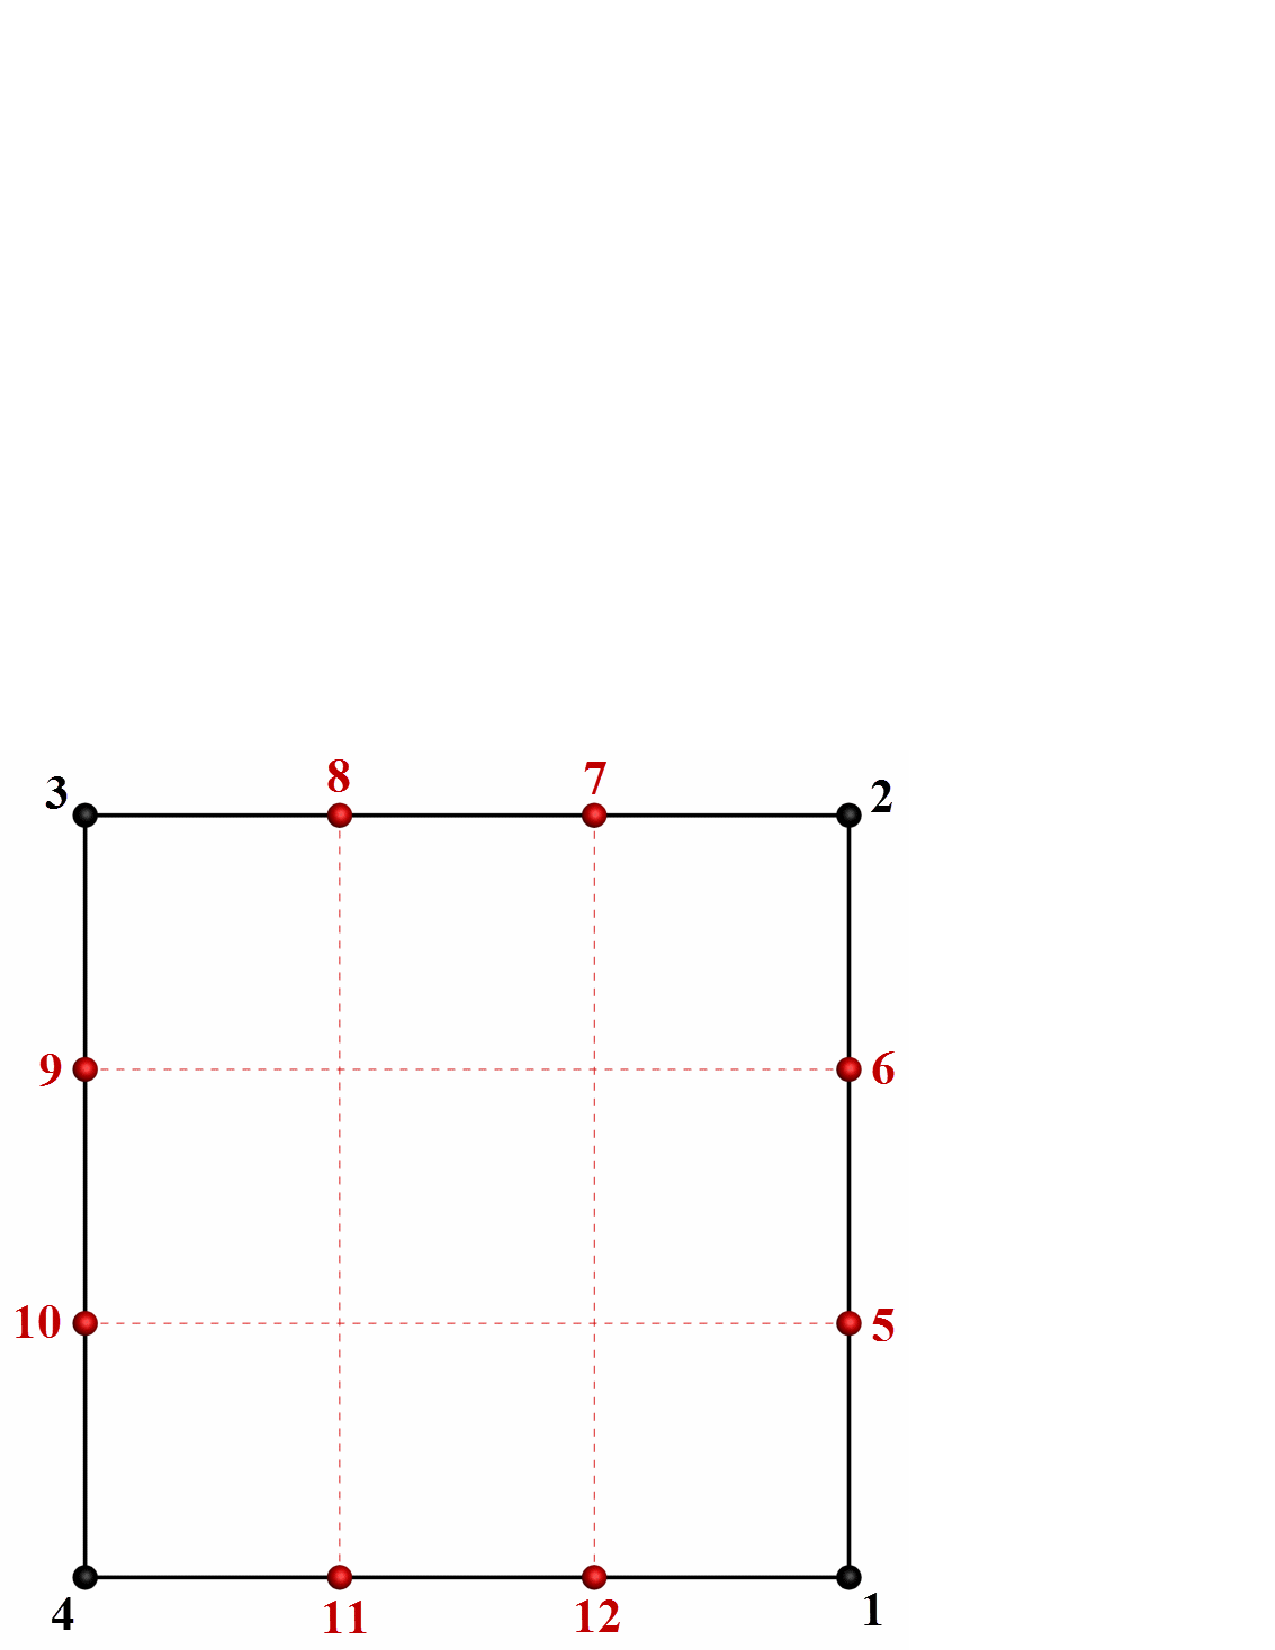
\includegraphics[width=2.5in]{conv.figs/TecplotFiles_Cubic_Element/All_Figures/quad_p3_12}
   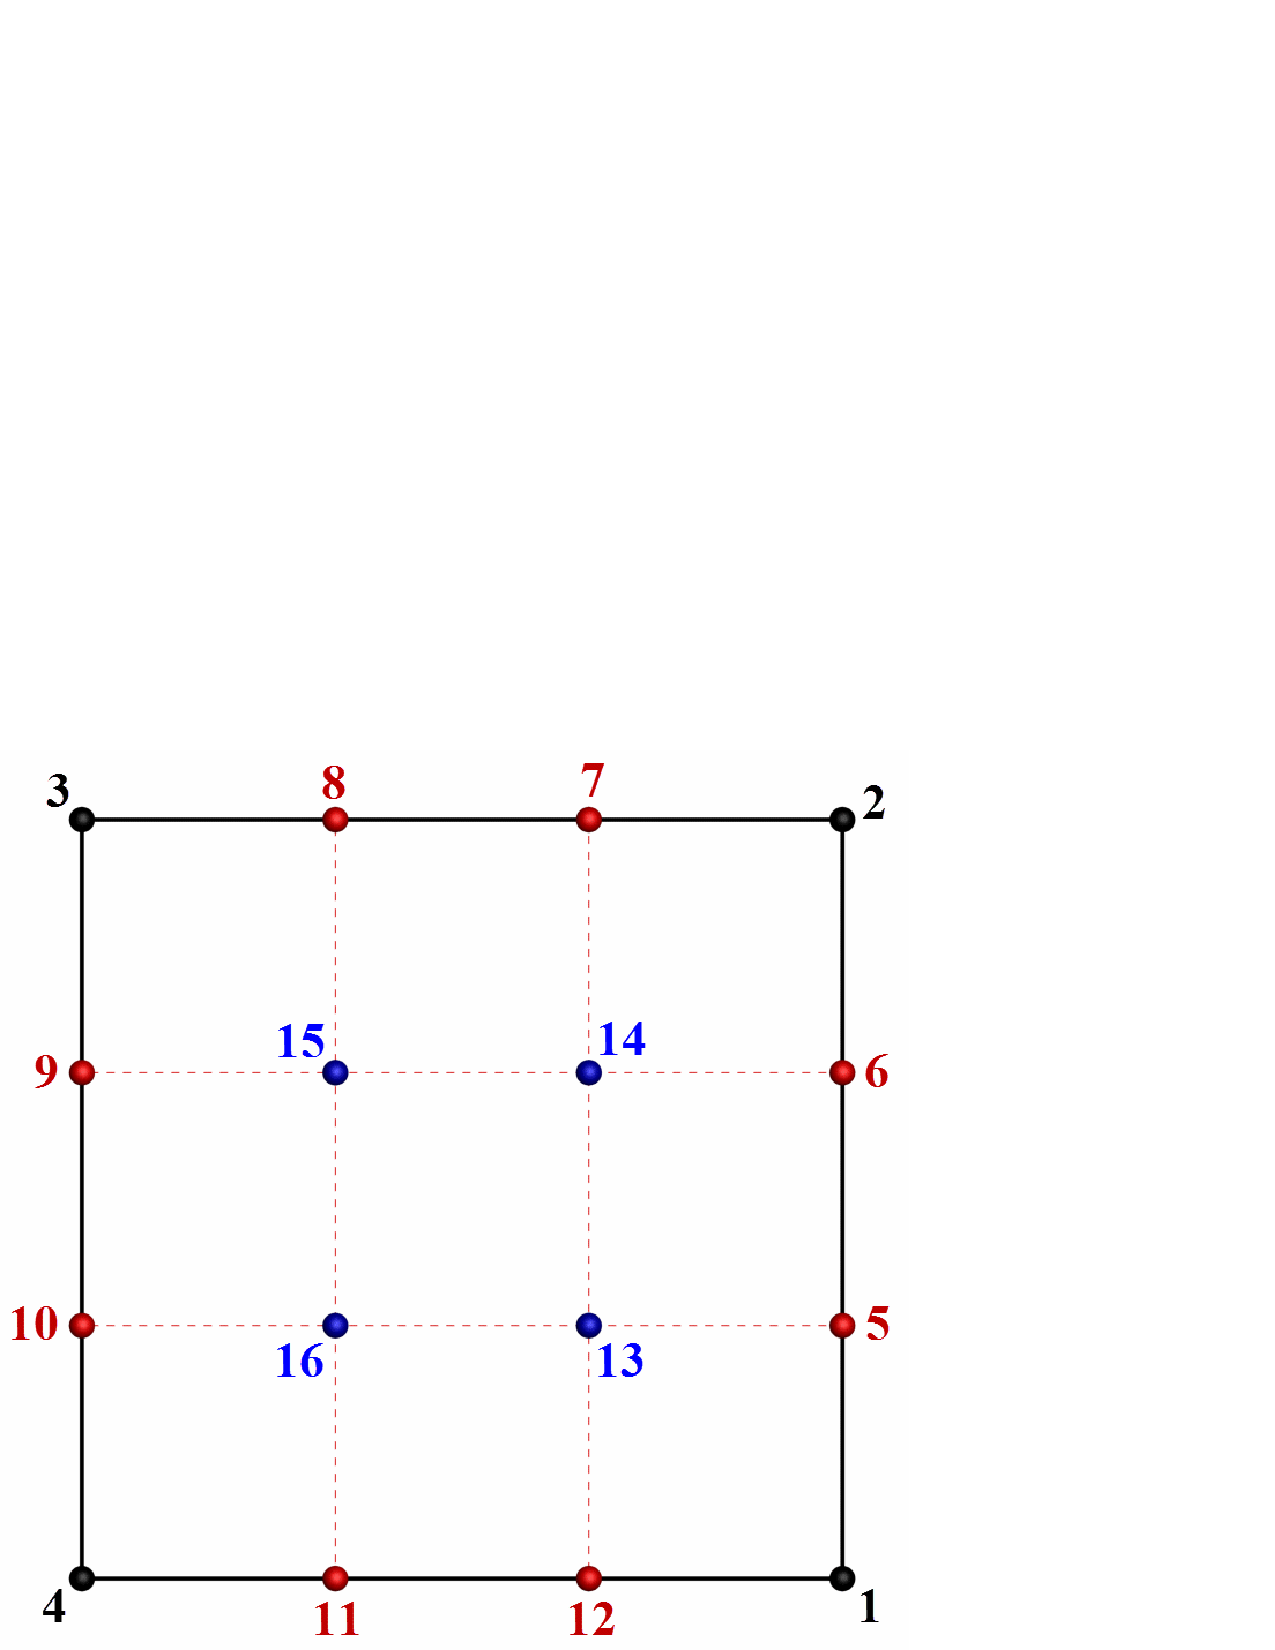
\includegraphics[width=2.5in]{conv.figs/TecplotFiles_Cubic_Element/All_Figures/quad_p3_16}
\end{figure}

\begin{minipage}[t]{0.5\linewidth}
   \vspace{0pt}
   \centering
   \begin{tabular}{@{}>{\ttfamily}l >{\ttfamily}l >{\ttfamily\color{red}}l}
      \multicolumn{3}{@{}l}{\uline{\textit{Edge Definition}}} \\[6pt]
      \textnormal{Oriented}      & \textnormal{Corner}        & \textnormal{Mid-} \\
      \uline{\textnormal{edges}} & \uline{\textnormal{nodes}} & \uline{\textnormal{node}} \\[3pt]
      E1  & N1,N2 & N5,N6 \\
      E2  & N2,N3 & N7,N8 \\
      E3  & N3,N4 & N9,N10 \\
      E4  & N4,N1 & N11,N12
   \end{tabular}
\end{minipage}

\medskip

\begin{tabular}{@{}>{\ttfamily}c >{\ttfamily}l >{\ttfamily\color{red}}l >{\ttfamily\color{blue}}c >{\ttfamily}l}
   \multicolumn{5}{@{}l}{\uline{\textit{Face Definition}}} \\[6pt]
   \uline{\textnormal{Face}} & \uline{\textnormal{Corner nodes}} & \uline{\textnormal{Mid-edge nodes}} & \uline{\textnormal{Mid-face node}} & \uline{\textnormal{Oriented edges}} \\[3pt]
   F1 & N1,N2,N3,N4 & N5,N6,N7,N8,N9,N10,N11,N12   & N13,N14,N15,N16 & E1,E2,E3,E4
\end{tabular}

\vspace{1.5\baselineskip}

\uline{\textit{Notes}}%
\begin{Ventryi}{\fort{N1,\ldots,N27}}
   \item [\fort{N1,\ldots,N16}]
         Grid point identification number.
         Integer $\ge 0$ or blank, and no two values may be the same.
         Grid points \fort{N1}\ldots\fort{N4} are in
         consecutive order about the quadrangle.
   \item [\fort{E1,\ldots,E4}]
         Edge identification number.
   \item [\fort{F1}]
         Face identification number.
\end{Ventryi}

\subsubsection{3-D (Volume) Elements}
\label{s:unstructgrid_3d}

3-D elements represent a volume in 3-D space, and constitute the cells
of a 3-D mesh.
CGNS supports four different shapes of 3-D elements --- tetrahedra,
pyramids, pentahedra, and hexahedra.

\paragraph{Tetrahedral Elements}
CGNS supports four types of tetrahedral elements, \fort{TETRA\_4},
\fort{TETRA\_10}, \fort{TETRA\_16}, and \fort{TETRA\_20}.
\fort{TETRA\_4} elements are composed of four nodes located at the
four geometric corners of the tetrahedron.
\fort{TETRA\_10} elements have six additional nodes, at the middle
of each of the six edges.
The cubic forms of tetrahedral elements, \fort{TETRA\_16} and \fort{TETRA\_20}
contain two interior nodes along each edge, and four interior face nodes
in the case of \fort{TETRA\_20}.

\underbar{Linear and Quadratic Elements:}

\begin{minipage}[t]{0.5\linewidth}
   \vspace{0pt}
   \centering
   \hspace*{\tmplength}\fort{TETRA\_4}\hfill\mbox{} \\[\baselineskip]
   \begin{picture}(2.0,1.75)
      \drawline(0.0,0.75)(1.125,0.0)(2.0,0.875)(1.0,1.75)(0.0,0.75)
      \drawline(1.125,0.0)(1.0,1.75)
      \dashline{0.05}(0.0,0.75)(2.0,0.875)
      \put( 0.00,  0.75 ){\circle*{0.1}}
      \put(-0.10,  0.75 ){\makebox(0,0)[r]{1}}
      \put( 1.125, 0.00 ){\circle*{0.1}}
      \put( 1.175,-0.05 ){\makebox(0,0)[lt]{2}}
      \put( 2.00,  0.875){\circle*{0.1}}
      \put( 2.10,  0.875){\makebox(0,0)[l]{3}}
      \put( 1.00,  1.75 ){\circle*{0.1}}
      \put( 1.05,  1.80 ){\makebox(0,0)[lb]{4}}
   \end{picture}
\end{minipage}%
\begin{minipage}[t]{0.5\linewidth}
   \vspace{0pt}
   \centering
   \hspace*{\tmplength}\fort{TETRA\_10}\hfill\mbox{} \\[\baselineskip]
   \begin{picture}(2.0,1.75)
      \drawline(0.0,0.75)(1.125,0.0)(2.0,0.875)(1.0,1.75)(0.0,0.75)
      \drawline(1.125,0.0)(1.0,1.75)
      \dashline{0.05}(0.0,0.75)(2.0,0.875)
      \put( 0.00,  0.75 ){\circle*{0.1}}
      \put(-0.10,  0.75 ){\makebox(0,0)[r]{1}}
      \put( 1.125, 0.00 ){\circle*{0.1}}
      \put( 1.175,-0.05 ){\makebox(0,0)[lt]{2}}
      \put( 2.00,  0.875){\circle*{0.1}}
      \put( 2.10,  0.875){\makebox(0,0)[l]{3}}
      \put( 1.00,  1.75 ){\circle*{0.1}}
      \put( 1.05,  1.80 ){\makebox(0,0)[lb]{4}}
      {\color{red}
       \dashline[25]{0.025}(0.5625,0.375)(1.5625,0.4375)(0.875,0.8047)(0.5625,0.375)
       \dashline[25]{0.025}(0.50,1.25)(1.0536,1.00)(1.50,1.3125)(0.50,1.25)
      }
      \put(0.5625,0.375 ){\color{red}\circle*{0.1}}
      \put(0.5125,0.325 ){\color{red}\makebox(0,0)[rt]{5}}
      \put(1.5625,0.4375){\color{red}\circle*{0.1}}
      \put(1.6125,0.3875){\color{red}\makebox(0,0)[lt]{6}}
      \put(0.875 ,0.8047){\color{red}\circle*{0.1}}
      \put(0.825 ,0.8547){\color{red}\makebox(0,0)[rb]{7}}
      \put(0.50  ,1.25  ){\color{red}\circle*{0.1}}
      \put(0.45  ,1.30  ){\color{red}\makebox(0,0)[rb]{8}}
      \put(1.0536,1.00  ){\color{red}\circle*{0.1}}
      \put(1.1536,1.00  ){\color{red}\makebox(0,0)[l]{9}}
      \put(1.50  ,1.3125){\color{red}\circle*{0.1}}
      \put(1.55  ,1.3625){\color{red}\makebox(0,0)[lb]{10}}
   \end{picture}
\end{minipage}

\vspace{1.5\baselineskip}

\begin{minipage}[t]{0.35\linewidth}
   \vspace{0pt}
   \begin{tabular}{@{}>{\ttfamily}l >{\ttfamily}l >{\ttfamily\color{red}}l}
      \multicolumn{3}{@{}l}{\uline{\textit{Edge Definition}}} \\[6pt]
      \textnormal{Oriented}      & \textnormal{Corner}	   & \textnormal{Mid-} \\
      \uline{\textnormal{edges}} & \uline{\textnormal{nodes}} & \uline{\textnormal{node}} \\[3pt]
      E1  & N1,N2 & N5  \\
      E2  & N2,N3 & N6  \\
      E3  & N3,N1 & N7  \\
      E4  & N1,N4 & N8  \\
      E5  & N2,N4 & N9  \\
      E6  & N3,N4 & N10
   \end{tabular}
\end{minipage}%
\begin{minipage}[t]{0.65\linewidth}
   \vspace{0pt}
   \begin{tabular}{@{}>{\ttfamily}c >{\ttfamily}l >{\ttfamily\color{red}}l >{\ttfamily}l}
      \multicolumn{4}{@{}l}{\uline{\textit{Face Definition}}} \\[6pt]
      \uline{\textnormal{Face}} & \uline{\textnormal{Corner nodes}} & \uline{\textnormal{Mid-edge nodes}} & \uline{\textnormal{Oriented edges}} \\[3pt]
      F1 & N1,N3,N2 & N7,N6,\ N5  & -E3,-E2,-E1   \\
      F2 & N1,N2,N4 & N5,N9,\ N8  & \ E1,\ E5,-E4 \\
      F3 & N2,N3,N4 & N6,N10,N9   & \ E2,\ E6,-E5 \\
      F4 & N3,N1,N4 & N7,N8,\ N10 & \ E3,\ E4,-E6
   \end{tabular}
\end{minipage}

\underbar{Cubic Elements:}

TETRA\_16
\begin{figure}[!htb]
%   \centering
   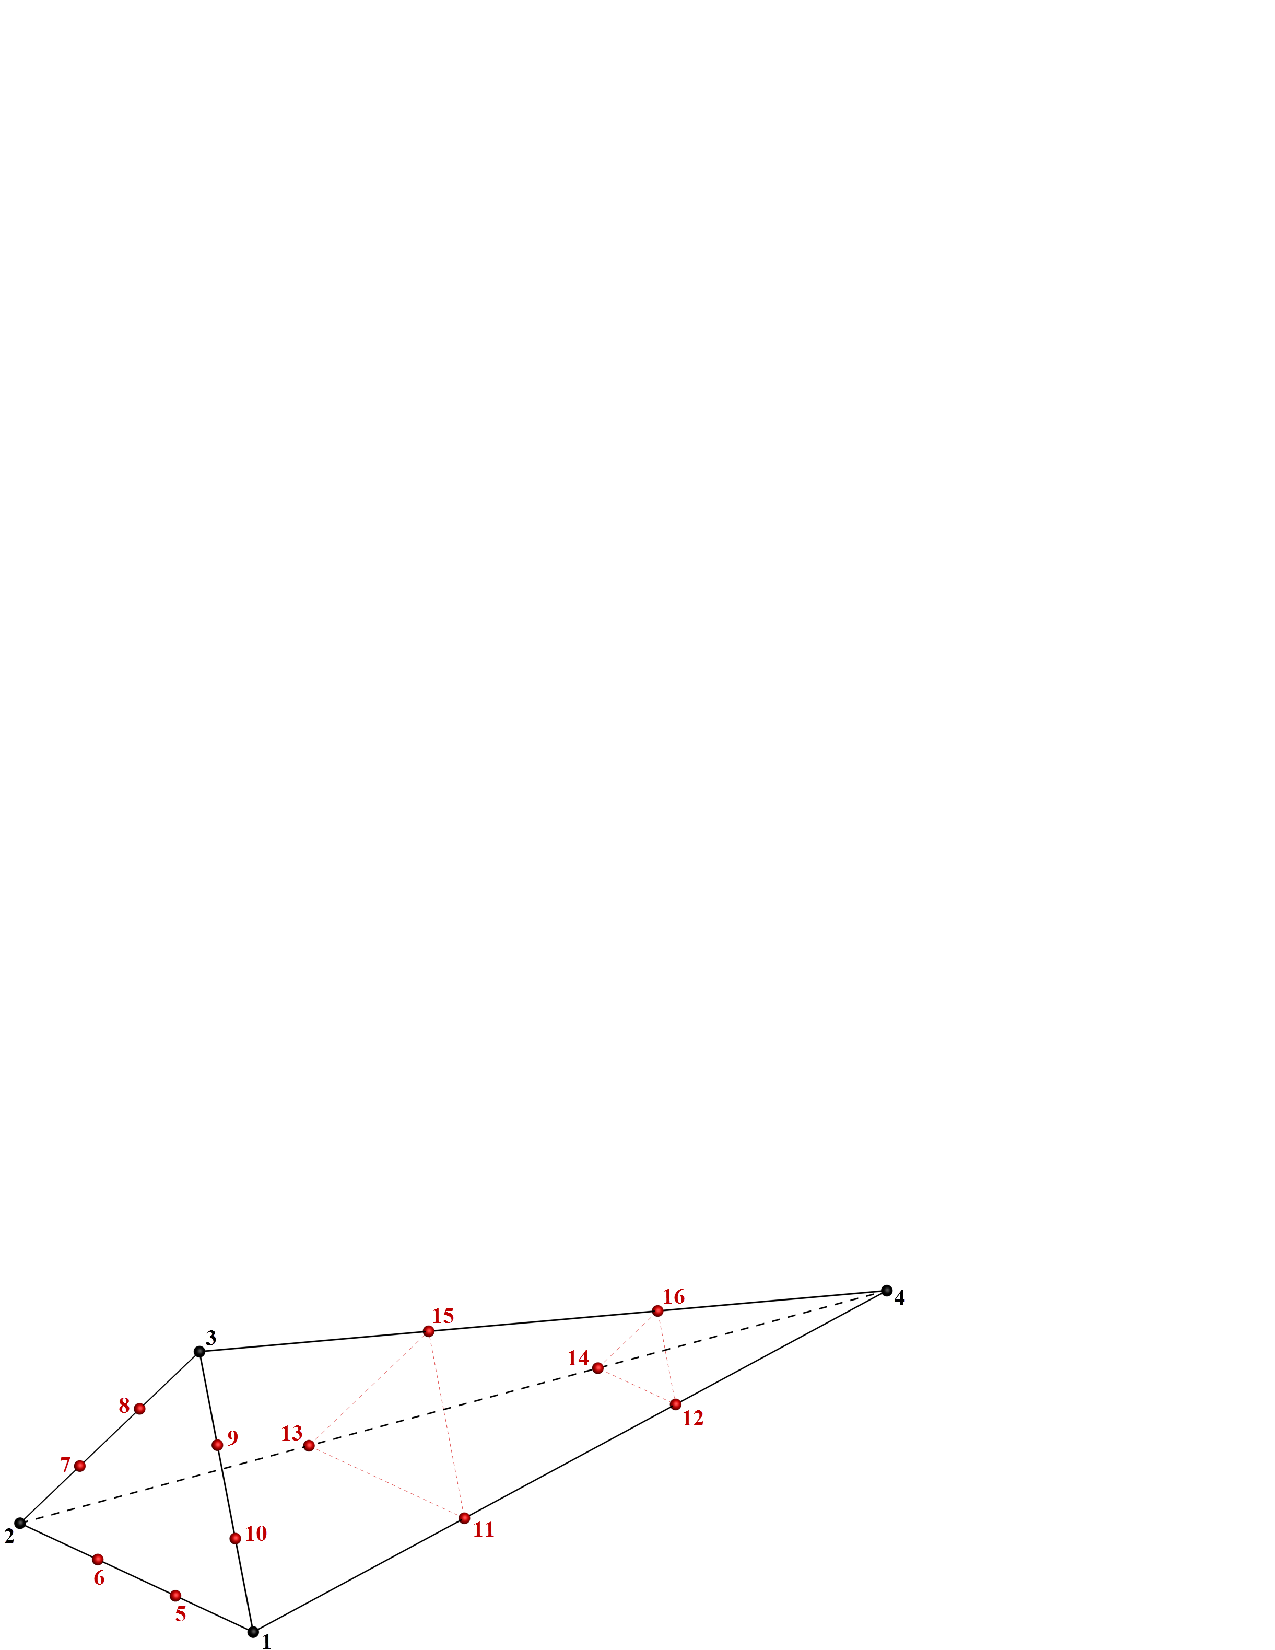
\includegraphics[width=4in]{conv.figs/TecplotFiles_Cubic_Element/All_Figures/tetra_16}
\end{figure}

\bigskip

TETRA\_20
\begin{figure}[!htb]
%   \centering
   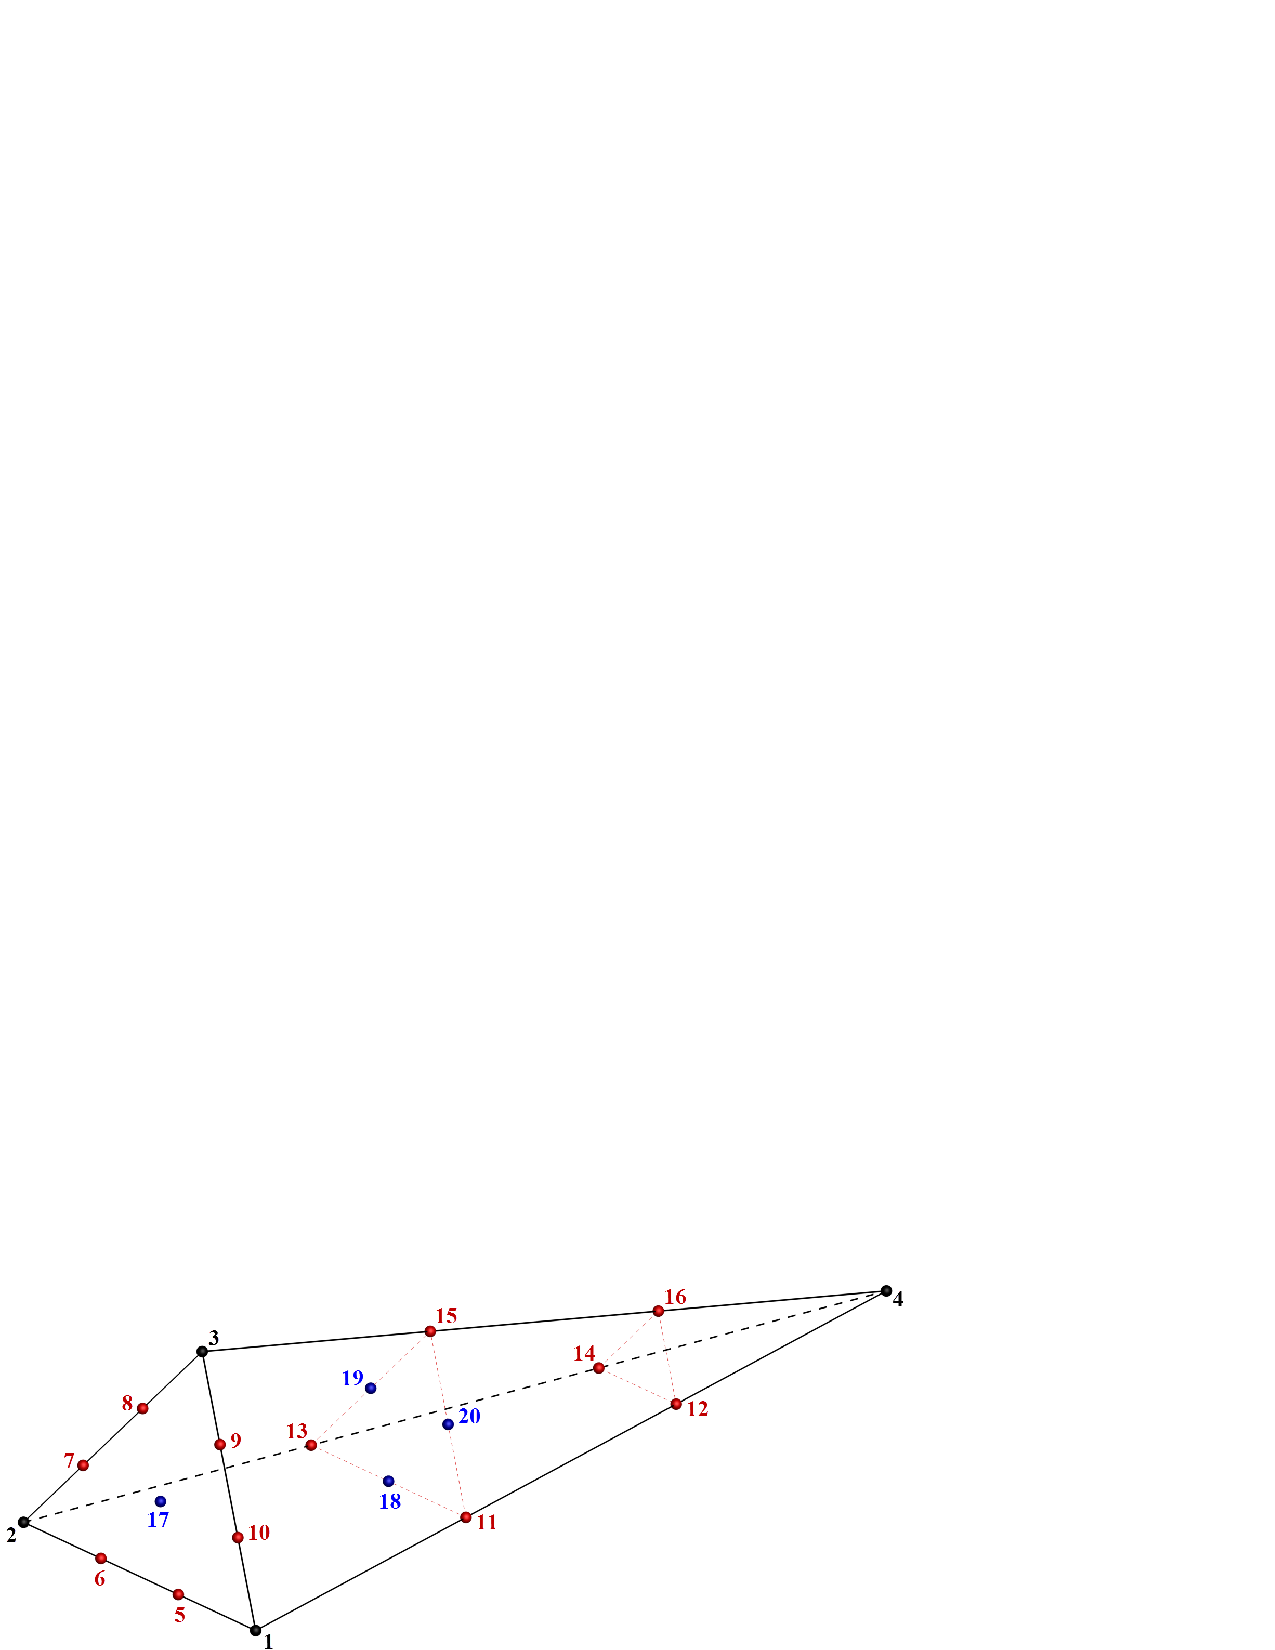
\includegraphics[width=4in]{conv.figs/TecplotFiles_Cubic_Element/All_Figures/tetra_20}
\end{figure}

\begin{minipage}[t]{0.35\linewidth}
   \vspace{0pt}
   \begin{tabular}{@{}>{\ttfamily}l >{\ttfamily}l >{\ttfamily\color{red}}l}
      \multicolumn{3}{@{}l}{\uline{\textit{Edge Definition}}} \\[6pt]
      \textnormal{Oriented}      & \textnormal{Corner}     & \textnormal{Mid-} \\
      \uline{\textnormal{edges}} & \uline{\textnormal{nodes}} & \uline{\textnormal{node}} \\[3pt]
      E1  & N1,N2 & N5,N6  \\
      E2  & N2,N3 & N7,N8  \\
      E3  & N3,N1 & N9,N10  \\
      E4  & N1,N4 & N11,N12  \\
      E5  & N2,N4 & N13,N14  \\
      E6  & N3,N4 & N15,N16
   \end{tabular}
\end{minipage}

\begin{minipage}[t]{0.65\linewidth}
   \vspace{0pt}
   \begin{tabular}{@{}>{\ttfamily}c >{\ttfamily}l >{\ttfamily\color{red}}l >{\ttfamily\color{blue}}l >{\ttfamily}l}
      \multicolumn{5}{@{}l}{\uline{\textit{Face Definition}}} \\[6pt]
      \uline{\textnormal{Face}} & \uline{\textnormal{Corner nodes}} & \uline{\textnormal{Mid-edge nodes}} & \uline{\textnormal{Mid-face node}} & \uline{\textnormal{Oriented edges}} \\[3pt]
      F1 & N1,N3,N2 & N10,N9,N8,N7,N6,N5     & N17 & -E3,-E2,-E1   \\
      F2 & N1,N2,N4 & N5,N6,N13,N14,N12,N11  & N18 & \ E1,\ E5,-E4 \\
      F3 & N2,N3,N4 & N7,N8,N15,N16,N14,N13  & N19 & \ E2,\ E6,-E5 \\
      F4 & N3,N1,N4 & N9,N10,N11,N12,N16,N15 & N20 & \ E3,\ E4,-E6
   \end{tabular}
\end{minipage}

\bigskip

\uline{\textit{Notes}}%
\begin{Ventryi}{\fort{N1,\ldots,N27}}
   \item [\fort{N1,\ldots,N20}]
         Grid point identification number.
         Integer $\ge 0$ or blank, and no two values may be the same.
         Grid points \fort{N1}\ldots\fort{N3} are in consecutive order about
         one trilateral face.
         The cross product of a vector going from \fort{N1} to \fort{N2},
         with a vector going from \fort{N1} to \fort{N3}, must result in a
         vector oriented from face \fort{F1} toward \fort{N4}.
   \item [\fort{E1,\ldots,E6}]
         Edge identification number.
         The edges are oriented from the first to the second node.
         A negative edge (e.g., \fort{-E1}) means that the edge is used in
         its reverse direction.
   \item [\fort{F1,\ldots,F4}]
         Face identification number.
         The faces are oriented so that the cross product of a vector
         from its first to second node, with a vector from its first to
         third node, is oriented outward.
\end{Ventryi}

\paragraph{Pyramid Elements}
CGNS supports six types of pyramid elements, \fort{PYRA\_5},
\texttt{PYRA\_13}, \texttt{PYRA\_14}, \texttt{PYRA\_21}, \texttt{PYRA\_29}, and \texttt{PYRA\_30}.
\fort{PYRA\_5} elements are composed of five nodes located at the
five geometric corners of the pyramid.
In addition, \texttt{PYRA\_13} and \texttt{PYRA\_14} elements have a node
at the middle of each of the eight edges; \texttt{PYRA\_14} adds a node
at the middle of the quadrilateral face.
The cubic forms of pyramid elements, \fort{PYRA\_21},
\fort{PYRA\_29}, and \fort{PYRA\_30}
contain two interior nodes along each edge, eight interior face nodes
in the case of \fort{PYRA\_29} and \fort{PYRA\_30}, and an additonal
interior volume node for \fort{PYRA\_30}.

\underbar{Linear and Quadratic Elements:}

\begin{minipage}[t]{0.5\linewidth}
   \vspace{0pt}
   \centering
   \hspace*{\tmplength}\fort{PYRA\_5}\hfill\mbox{} \\[\baselineskip]
   \begin{picture}(2.0,2.125)
      \drawline(1.375,2.125)(0.0,0.875)(0.5,0.0)(2.0,0.125)(1.375,2.125)(0.5,0.0)
      \dashline{0.05}(0.0,0.875)(1.375,1.0)(2.0,0.125)
      \dashline{0.05}(1.375,2.125)(1.375,1.0)
      \put( 0.50,  0.00 ){\circle*{0.1}}
      \put( 0.45, -0.05 ){\makebox(0,0)[rt]{1}}
      \put( 2.00,  0.125){\circle*{0.1}}
      \put( 2.05,  0.075){\makebox(0,0)[lt]{2}}
      \put( 1.375, 1.00 ){\circle*{0.1}}
      \put( 1.475, 1.00 ){\makebox(0,0)[l]{3}}
      \put( 0.00,  0.875){\circle*{0.1}}
      \put(-0.05,  0.825){\makebox(0,0)[rt]{4}}
      \put( 1.375, 2.125){\circle*{0.1}}
      \put( 1.425, 2.175){\makebox(0,0)[lb]{5}}
   \end{picture}
\end{minipage}%
\begin{minipage}[t]{0.5\linewidth}
   \vspace{0pt}
   \centering
   \hspace*{\tmplength}\fort{PYRA\_13}\hfill\mbox{} \\[\baselineskip]
   \begin{picture}(2.0,2.125)
      \drawline(1.375,2.125)(0.0,0.875)(0.5,0.0)(2.0,0.125)(1.375,2.125)(0.5,0.0)
      \dashline{0.05}(0.0,0.875)(1.375,1.0)(2.0,0.125)
      \dashline{0.05}(1.375,2.125)(1.375,1.0)
      \put( 0.50,  0.00 ){\circle*{0.1}}
      \put( 0.45, -0.05 ){\makebox(0,0)[rt]{1}}
      \put( 2.00,  0.125){\circle*{0.1}}
      \put( 2.05,  0.075){\makebox(0,0)[lt]{2}}
      \put( 1.375, 1.00 ){\circle*{0.1}}
      \put( 1.475, 1.00 ){\makebox(0,0)[l]{3}}
      \put( 0.00,  0.875){\circle*{0.1}}
      \put(-0.05,  0.825){\makebox(0,0)[rt]{4}}
      \put( 1.375, 2.125){\circle*{0.1}}
      \put( 1.425, 2.175){\makebox(0,0)[lb]{5}}
      {\color{red}
       \dashline[25]{0.025}(1.25,0.0625)(0.6875,0.9375)
       \dashline[25]{0.025}(0.25,0.4375)(1.6875,0.5625)
       \dashline[25]{0.025}(0.9375,1.0625)(1.6875,1.125)(1.375,1.5625)(0.6875,1.5)(0.9375,1.0625)
      }
      \put(1.25,  0.0625){\color{red}\circle*{0.1}}
      \put(1.30,  0.0125){\color{red}\makebox(0,0)[lt]{6}}
      \put(1.6875,0.5625){\color{red}\circle*{0.1}}
      \put(1.6375,0.5125){\color{red}\makebox(0,0)[rt]{7}}
      \put(0.6875,0.9375){\color{red}\circle*{0.1}}
      \put(0.6375,0.9875){\color{red}\makebox(0,0)[rb]{8}}
      \put(0.25,  0.4375){\color{red}\circle*{0.1}}
      \put(0.20,  0.3875){\color{red}\makebox(0,0)[rt]{9}}
      \put(0.9375,1.0625){\color{red}\circle*{0.1}}
      \put(0.9875,1.1125){\color{red}\makebox(0,0)[lb]{10}}
      \put(1.6875,1.125 ){\color{red}\circle*{0.1}}
      \put(1.7375,1.175 ){\color{red}\makebox(0,0)[lb]{11}}
      \put(1.375, 1.5625){\color{red}\circle*{0.1}}
      \put(1.325, 1.5125){\color{red}\makebox(0,0)[rt]{12}}
      \put(0.6875,1.5   ){\color{red}\circle*{0.1}}
      \put(0.6375,1.55  ){\color{red}\makebox(0,0)[rb]{13}}
   \end{picture}
\end{minipage}

\vspace{1.5\baselineskip}

\begin{minipage}[t]{0.5\linewidth}
   \vspace{0pt}
   \centering
   \hspace*{\tmplength}\fort{PYRA\_14}\hfill\mbox{} \\[\baselineskip]
   \begin{picture}(2.0,2.125)
      \drawline(1.375,2.125)(0.0,0.875)(0.5,0.0)(2.0,0.125)(1.375,2.125)(0.5,0.0)
      \dashline{0.05}(0.0,0.875)(1.375,1.0)(2.0,0.125)
      \dashline{0.05}(1.375,2.125)(1.375,1.0)
      \put( 0.50,  0.00 ){\circle*{0.1}}
      \put( 0.45, -0.05 ){\makebox(0,0)[rt]{1}}
      \put( 2.00,  0.125){\circle*{0.1}}
      \put( 2.05,  0.075){\makebox(0,0)[lt]{2}}
      \put( 1.375, 1.00 ){\circle*{0.1}}
      \put( 1.475, 1.00 ){\makebox(0,0)[l]{3}}
      \put( 0.00,  0.875){\circle*{0.1}}
      \put(-0.05,  0.825){\makebox(0,0)[rt]{4}}
      \put( 1.375, 2.125){\circle*{0.1}}
      \put( 1.425, 2.175){\makebox(0,0)[lb]{5}}
      {\color{red}
       \dashline[25]{0.025}(1.25,0.0625)(0.6875,0.9375)
       \dashline[25]{0.025}(0.25,0.4375)(1.6875,0.5625)
       \dashline[25]{0.025}(0.9375,1.0625)(1.6875,1.125)(1.375,1.5625)(0.6875,1.5)(0.9375,1.0625)
      }
      \put(1.25,  0.0625){\color{red}\circle*{0.1}}
      \put(1.30,  0.0125){\color{red}\makebox(0,0)[lt]{6}}
      \put(1.6875,0.5625){\color{red}\circle*{0.1}}
      \put(1.6375,0.5125){\color{red}\makebox(0,0)[rt]{7}}
      \put(0.6875,0.9375){\color{red}\circle*{0.1}}
      \put(0.6375,0.9875){\color{red}\makebox(0,0)[rb]{8}}
      \put(0.25,  0.4375){\color{red}\circle*{0.1}}
      \put(0.20,  0.3875){\color{red}\makebox(0,0)[rt]{9}}
      \put(0.9375,1.0625){\color{red}\circle*{0.1}}
      \put(0.9875,1.1125){\color{red}\makebox(0,0)[lb]{10}}
      \put(1.6875,1.125 ){\color{red}\circle*{0.1}}
      \put(1.7375,1.175 ){\color{red}\makebox(0,0)[lb]{11}}
      \put(1.375, 1.5625){\color{red}\circle*{0.1}}
      \put(1.325, 1.5125){\color{red}\makebox(0,0)[rt]{12}}
      \put(0.6875,1.5   ){\color{red}\circle*{0.1}}
      \put(0.6375,1.55  ){\color{red}\makebox(0,0)[rb]{13}}
      \put(0.96875, 0.5 ){\color{blue}\circle*{0.1}}
      \put(0.91875, 0.45){\color{blue}\makebox(0,0)[rt]{14}}
   \end{picture}
\end{minipage}%
\begin{minipage}[t]{0.5\linewidth}
   \vspace{0pt}
   \centering
   \begin{tabular}{@{}>{\ttfamily}l >{\ttfamily}l >{\ttfamily\color{red}}l}
      \multicolumn{3}{@{}l}{\uline{\textit{Edge Definition}}} \\[6pt]
      \textnormal{Oriented}      & \textnormal{Corner}        & \textnormal{Mid-} \\
      \uline{\textnormal{edges}} & \uline{\textnormal{nodes}} & \uline{\textnormal{node}} \\[3pt]
      E1  & N1,N2 & N6  \\
      E2  & N2,N3 & N7  \\
      E3  & N3,N4 & N8  \\
      E4  & N4,N1 & N9  \\
      E5  & N1,N5 & N10 \\
      E6  & N2,N5 & N11 \\
      E7  & N3,N5 & N12 \\
      E8  & N4,N5 & N13
   \end{tabular}
\end{minipage}

\medskip

\begin{tabular}{@{}>{\ttfamily}c >{\ttfamily}l >{\ttfamily\color{red}}l >{\ttfamily\color{blue}}c >{\ttfamily}l}
   \multicolumn{5}{@{}l}{\uline{\textit{Face Definition}}} \\[6pt]
   \uline{\textnormal{Face}} & \uline{\textnormal{Corner nodes}} & \uline{\textnormal{Mid-edge nodes}} & \uline{\textnormal{Mid-face node}} & \uline{\textnormal{Oriented edges}} \\[3pt]
   F1 & N1,N4,N3,N2 & N9,N8,\ N7,\ N6  & N14 & -E4,-E3,-E2,-E1 \\
   F2 & N1,N2,N5    & N6,N11,N10       &     & \ E1,\ E6,-E5   \\
   F3 & N2,N3,N5    & N7,N12,N11       &     & \ E2,\ E7,-E6   \\
   F4 & N3,N4,N5    & N8,N13,N12       &     & \ E3,\ E8,-E7   \\
   F5 & N4,N1,N5    & N9,N10,N13       &     & \ E4,\ E5,-E8
\end{tabular}

\underbar{Cubic Elements:}

PYRA\_21
\begin{figure}[!htb]
%   \centering
   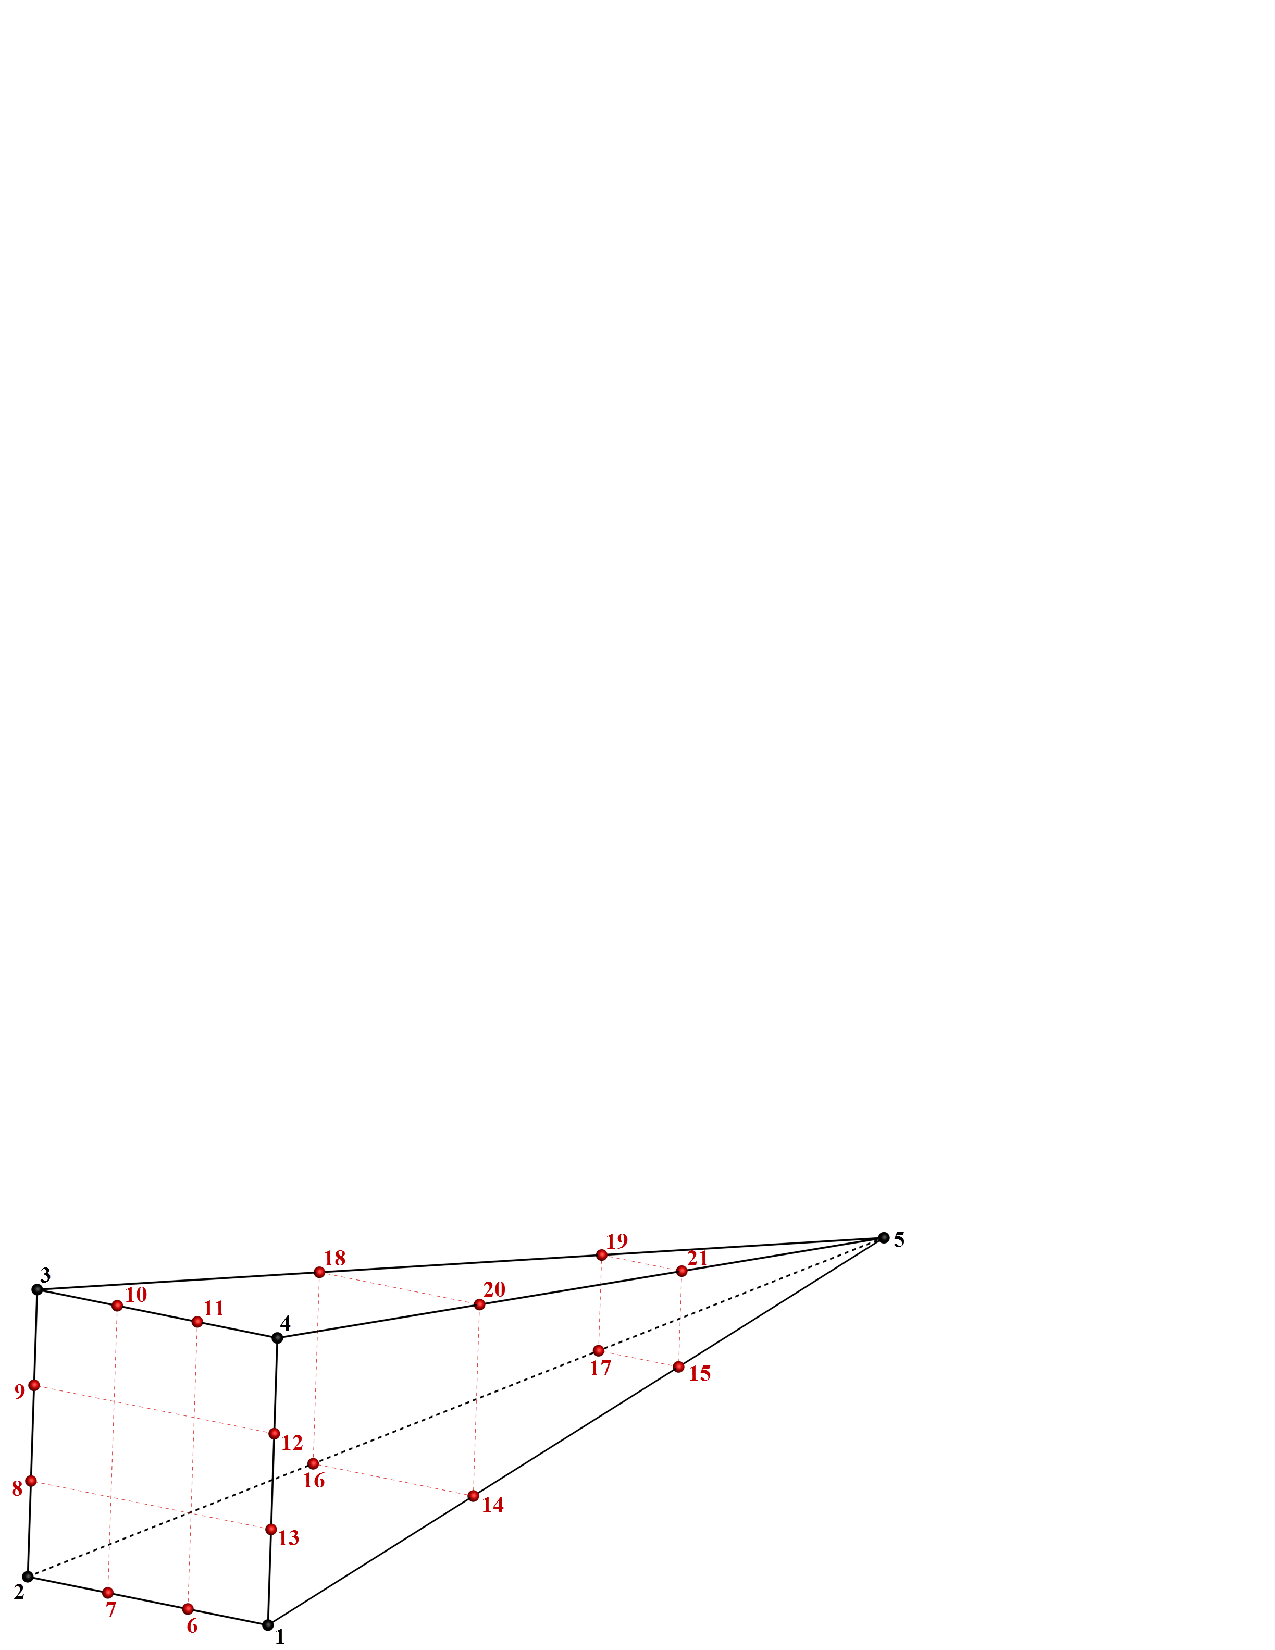
\includegraphics[width=4in]{conv.figs/TecplotFiles_Cubic_Element/All_Figures/pyramid_21}
\end{figure}

\bigskip

PYRA\_29
\begin{figure}[!htb]
%   \centering
   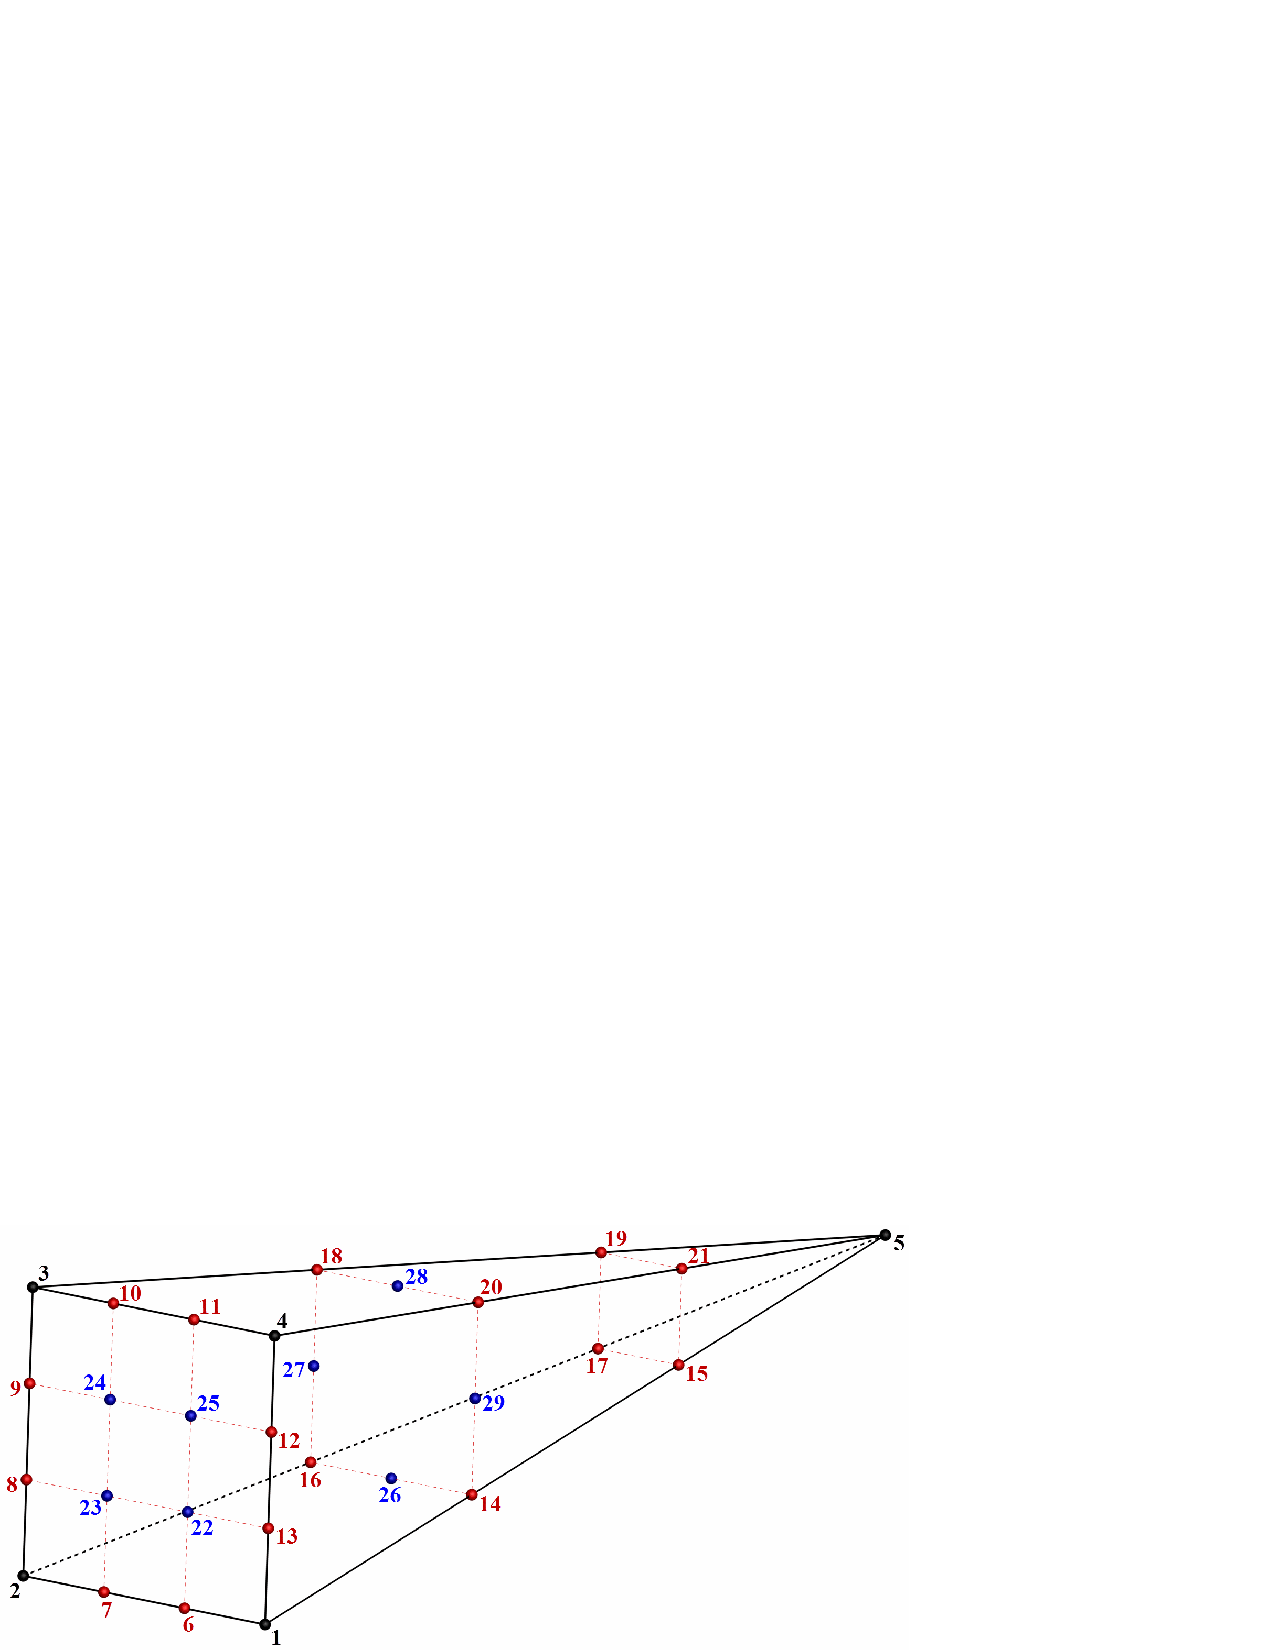
\includegraphics[width=4in]{conv.figs/TecplotFiles_Cubic_Element/All_Figures/pyramid_29}
\end{figure}

\newpage
PYRA\_30
\begin{figure}[!htb]
%   \centering
   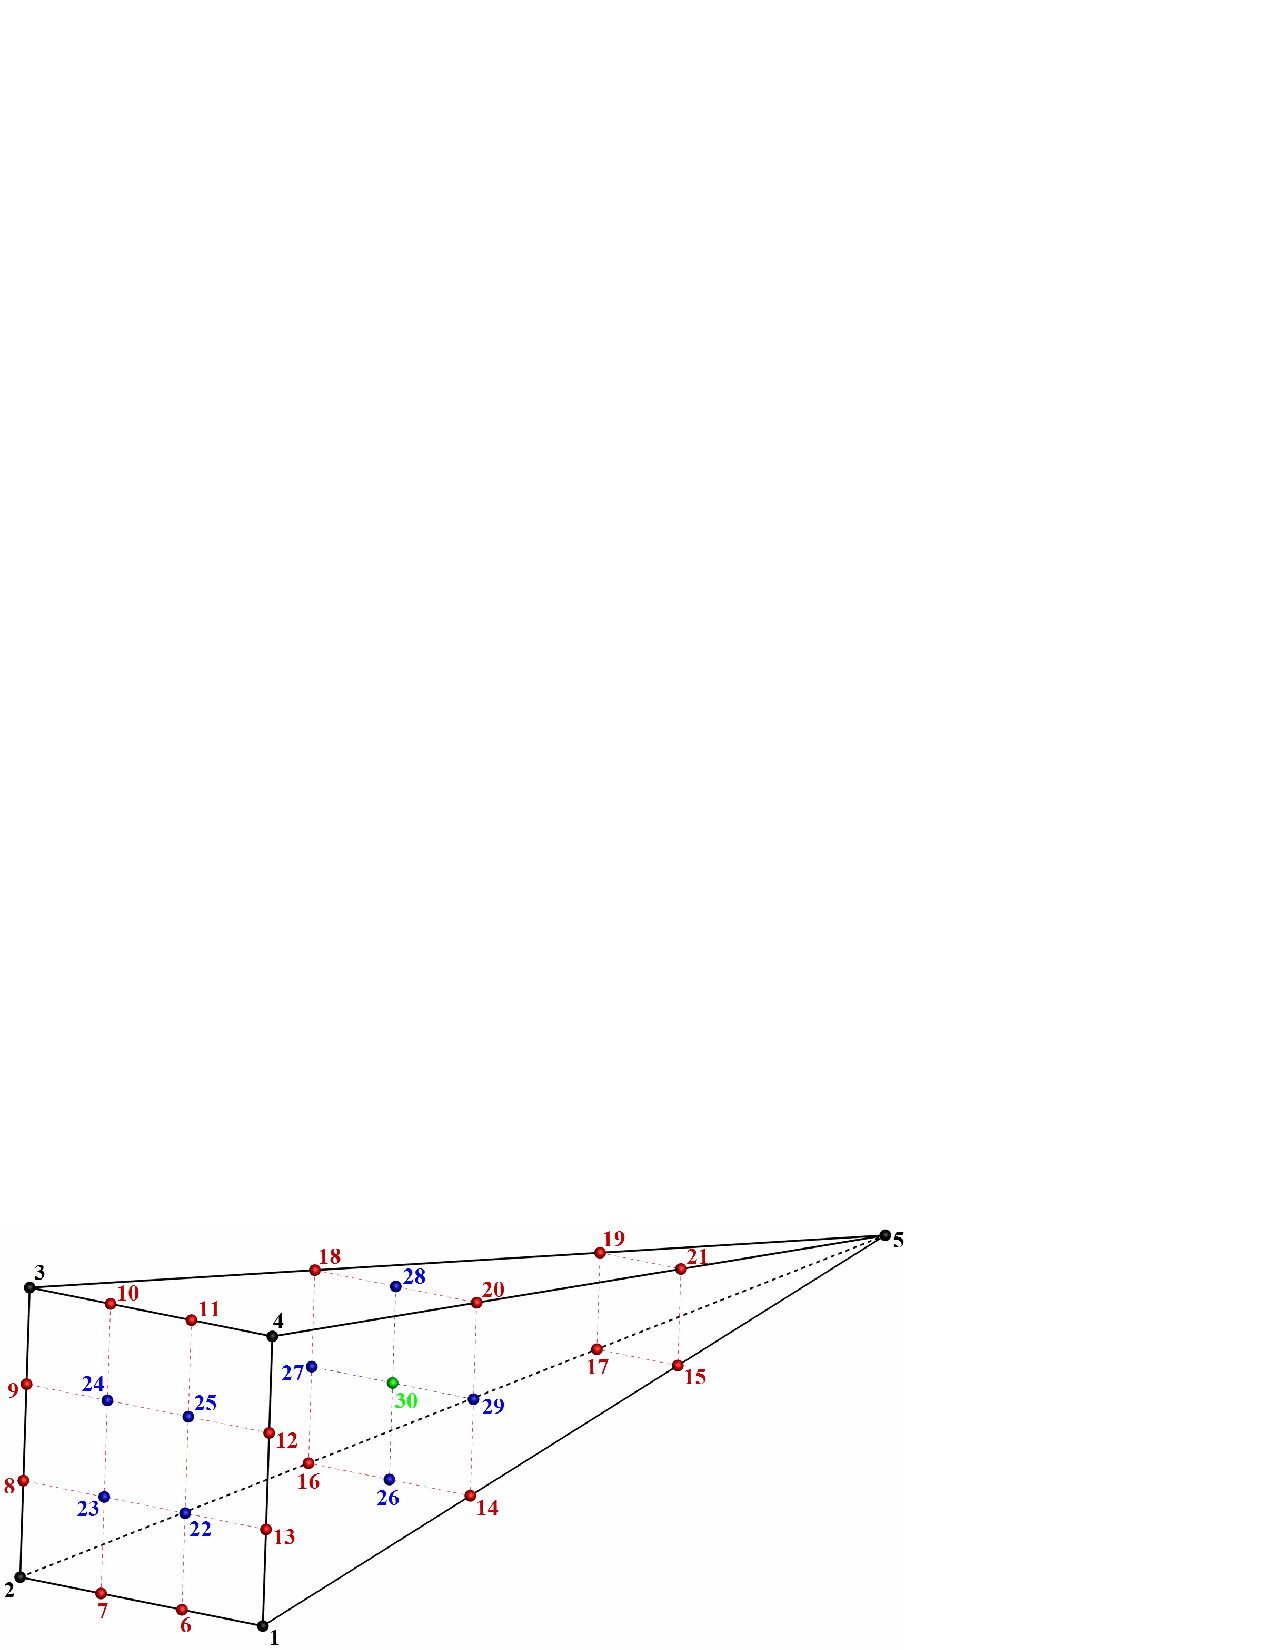
\includegraphics[width=4in]{conv.figs/TecplotFiles_Cubic_Element/All_Figures/pyramid_30}
\end{figure}

\begin{minipage}[t]{0.5\linewidth}
   \vspace{0pt}
   \centering
   \begin{tabular}{@{}>{\ttfamily}l >{\ttfamily}l >{\ttfamily\color{red}}l}
      \multicolumn{3}{@{}l}{\uline{\textit{Edge Definition}}} \\[6pt]
      \textnormal{Oriented}      & \textnormal{Corner}        & \textnormal{Mid-} \\
      \uline{\textnormal{edges}} & \uline{\textnormal{nodes}} & \uline{\textnormal{node}} \\[3pt]
      E1  & N1,N2 & N6,N7  \\
      E2  & N2,N3 & N8,N9  \\
      E3  & N3,N4 & N10,N11  \\
      E4  & N4,N1 & N12,N13  \\
      E5  & N1,N5 & N14,N15 \\
      E6  & N2,N5 & N16,N17 \\
      E7  & N3,N5 & N18,N19 \\
      E8  & N4,N5 & N20,N21
   \end{tabular}
\end{minipage}

\medskip

\begin{tabular}{@{}>{\ttfamily}c >{\ttfamily}l >{\ttfamily\color{red}}l >{\ttfamily\color{blue}}c >{\ttfamily}l}
   \multicolumn{5}{@{}l}{\uline{\textit{Face Definition}}} \\[6pt]
   \uline{\textnormal{Face}} & \uline{\textnormal{Corner nodes}} & \uline{\textnormal{Mid-edge nodes}} & \uline{\textnormal{Mid-face node}} & \uline{\textnormal{Oriented edges}} \\[3pt]
   F1 & N1,N4,N3,N2 & N13,N12,N11,N10,N9,N8,N7,N6  & N22,N25,N24,N23 & -E4,-E3,-E2,-E1 \\
   F2 & N1,N2,N5    & N6,N7,N16,N17,N15,N14        & N26    & \ E1,\ E6,-E5   \\
   F3 & N2,N3,N5    & N8,N9,N18,N19,N17,N16        & N27    & \ E2,\ E7,-E6   \\
   F4 & N3,N4,N5    & N10,N11,N20,N21,N19,N18      & N28    & \ E3,\ E8,-E7   \\
   F5 & N4,N1,N5    & N12,N13,N14,N15,N21,N20      & N29    & \ E4,\ E5,-E8
\end{tabular}

\bigskip

\uline{\textit{Notes}}%
\begin{Ventryi}{\fort{N1,\ldots,N27}}
   \item [\fort{N1,\ldots,N30}]
         Grid point identification number.
         Integer $\ge 0$ or blank, and no two values may be the same.
         Grid points \fort{N1}\ldots\fort{N4} are in consecutive order about
         the quadrilateral face.
         The cross product of a vector going from \fort{N1} to \fort{N2},
         with a vector going from \fort{N1} to \fort{N3}, must result in a
         vector oriented from face \fort{F1} toward \fort{N5}.
   \item [\fort{E1,\ldots,E8}]
         Edge identification number.
         The edges are oriented from the first to the second node.
         A negative edge (e.g., \fort{-E1}) means that the edge is used in
         its reverse direction.
   \item [\fort{F1,\ldots,F5}]
         Face identification number.
         The faces are oriented so that the cross product of a vector
         from its first to second node, with a vector from its first to
         third node, is oriented outward.
\end{Ventryi}

\paragraph{Pentahedral Elements}
CGNS supports six types of pentahedral elements, \fort{PENTA\_6},
\fort{PENTA\_15}, \fort{PENTA\_18}, \fort{PENTA\_24}, \fort{PENTA\_38}, and \fort{PENTA\_40}.
\fort{PENTA\_6} elements are composed of six nodes located at the
six geometric corners of the pentahedron.
In addition, \fort{PENTA\_15} and \fort{PENTA\_18} elements have a node
at the middle of each of the nine edges; \fort{PENTA\_18} adds a
node at the middle of each of the three quadrilateral faces.
The cubic forms of the pentahedral elements, \fort{PENTA\_24},
\fort{PENTA\_38}, and \fort{PENTA\_40}
contain two interior nodes along each edge, fourteen interior face nodes
in the case of \fort{PENTA\_38} and \fort{PENTA\_40}, and an additonal
two interior volume nodes for \fort{PENTA\_40}.

\underbar{Linear and Quadratic Elements:}

\begin{minipage}[t]{0.5\linewidth}
   \vspace{0pt}
   \centering
   \hspace*{\tmplength}\fort{PENTA\_6}\hfill\mbox{} \\[\baselineskip]
   \begin{picture}(2.0,2.75)
      \drawline(0.0,0.0)(2.0,0.0)(2.0,2.0)(0.0,2.0)(0.0,0.0)
      \drawline(0.0,2.0)(1.0,2.75)(2.0,2.0)
      \dashline{0.05}(0.0,0.0)(1.0,0.75)(2.0,0.0)
      \dashline{0.05}(1.0,0.75)(1.0,2.75)
      \put( 0.00, 0.00){\circle*{0.1}}
      \put(-0.05,-0.05){\makebox(0,0)[rt]{1}}
      \put( 2.00, 0.00){\circle*{0.1}}
      \put( 2.05,-0.05){\makebox(0,0)[lt]{2}}
      \put( 1.00, 0.75){\circle*{0.1}}
      \put( 0.90, 0.75){\makebox(0,0)[r]{3}}
      \put( 0.00, 2.00){\circle*{0.1}}
      \put(-0.05, 2.05){\makebox(0,0)[rb]{4}}
      \put( 2.00, 2.00){\circle*{0.1}}
      \put( 2.05, 2.05){\makebox(0,0)[lb]{5}}
      \put( 1.00, 2.75){\circle*{0.1}}
      \put( 1.05, 2.80){\makebox(0,0)[lb]{6}}
   \end{picture}
\end{minipage}%
\begin{minipage}[t]{0.5\linewidth}
   \vspace{0pt}
   \centering
   \hspace*{\tmplength}\fort{PENTA\_15}\hfill\mbox{} \\[\baselineskip]
   \begin{picture}(2.0,2.75)
      \drawline(0.0,0.0)(2.0,0.0)(2.0,2.0)(0.0,2.0)(0.0,0.0)
      \drawline(0.0,2.0)(1.0,2.75)(2.0,2.0)
      \dashline{0.05}(0.0,0.0)(1.0,0.75)(2.0,0.0)
      \dashline{0.05}(1.0,0.75)(1.0,2.75)
      \put( 0.00, 0.00){\circle*{0.1}}
      \put(-0.05,-0.05){\makebox(0,0)[rt]{1}}
      \put( 2.00, 0.00){\circle*{0.1}}
      \put( 2.05,-0.05){\makebox(0,0)[lt]{2}}
      \put( 1.00, 0.75){\circle*{0.1}}
      \put( 0.90, 0.75){\makebox(0,0)[r]{3}}
      \put( 0.00, 2.00){\circle*{0.1}}
      \put(-0.05, 2.05){\makebox(0,0)[rb]{4}}
      \put( 2.00, 2.00){\circle*{0.1}}
      \put( 2.05, 2.05){\makebox(0,0)[lb]{5}}
      \put( 1.00, 2.75){\circle*{0.1}}
      \put( 1.05, 2.80){\makebox(0,0)[lb]{6}}
      {\color{red}
       \dashline[25]{0.025}(1.00,0.00)(1.50,0.375)(0.50,0.375)(1.00,0.00)
       \dashline[25]{0.025}(0.00,1.00)(2.00,1.00)(1.00,1.75)(0.00,1.00)
       \dashline[25]{0.025}(1.00,2.00)(1.50,2.375)(0.50,2.375)(1.00,2.00)
      }
      \put( 1.00, 0.00 ){\color{red}\circle*{0.1}}
      \put( 0.95,-0.05 ){\color{red}\makebox(0,0)[rt]{7}}
      \put( 1.50, 0.375){\color{red}\circle*{0.1}}
      \put( 1.55, 0.425){\color{red}\makebox(0,0)[lb]{8}}
      \put( 0.50, 0.375){\color{red}\circle*{0.1}}
      \put( 0.45, 0.425){\color{red}\makebox(0,0)[rb]{9}}
      \put( 0.00, 1.00 ){\color{red}\circle*{0.1}}
      \put(-0.10, 1.00 ){\color{red}\makebox(0,0)[r]{10}}
      \put( 2.00, 1.00 ){\color{red}\circle*{0.1}}
      \put( 2.10, 1.00 ){\color{red}\makebox(0,0)[l]{11}}
      \put( 1.00, 1.75 ){\color{red}\circle*{0.1}}
      \put( 1.05, 1.80 ){\color{red}\makebox(0,0)[lb]{12}}
      \put( 1.00, 2.00 ){\color{red}\circle*{0.1}}
      \put( 0.95, 1.95 ){\color{red}\makebox(0,0)[rt]{13}}
      \put( 1.50, 2.375){\color{red}\circle*{0.1}}
      \put( 1.55, 2.425){\color{red}\makebox(0,0)[lb]{14}}
      \put( 0.50, 2.375){\color{red}\circle*{0.1}}
      \put( 0.45, 2.425){\color{red}\makebox(0,0)[rb]{15}}
   \end{picture}
\end{minipage}

\vspace{1.5\baselineskip}

\begin{minipage}[t]{0.5\linewidth}
   \vspace{0pt}
   \centering
   \hspace*{\tmplength}\fort{PENTA\_18}\hfill\mbox{} \\[\baselineskip]
   \begin{picture}(2.0,2.75)
      \drawline(0.0,0.0)(2.0,0.0)(2.0,2.0)(0.0,2.0)(0.0,0.0)
      \drawline(0.0,2.0)(1.0,2.75)(2.0,2.0)
      \dashline{0.05}(0.0,0.0)(1.0,0.75)(2.0,0.0)
      \dashline{0.05}(1.0,0.75)(1.0,2.75)
      \put( 0.00, 0.00){\circle*{0.1}}
      \put(-0.05,-0.05){\makebox(0,0)[rt]{1}}
      \put( 2.00, 0.00){\circle*{0.1}}
      \put( 2.05,-0.05){\makebox(0,0)[lt]{2}}
      \put( 1.00, 0.75){\circle*{0.1}}
      \put( 0.90, 0.75){\makebox(0,0)[r]{3}}
      \put( 0.00, 2.00){\circle*{0.1}}
      \put(-0.05, 2.05){\makebox(0,0)[rb]{4}}
      \put( 2.00, 2.00){\circle*{0.1}}
      \put( 2.05, 2.05){\makebox(0,0)[lb]{5}}
      \put( 1.00, 2.75){\circle*{0.1}}
      \put( 1.05, 2.80){\makebox(0,0)[lb]{6}}
      {\color{red}
       \dashline[25]{0.025}(1.00,0.00)(1.50,0.375)(0.50,0.375)(1.00,0.00)
       \dashline[25]{0.025}(0.00,1.00)(2.00,1.00)(1.00,1.75)(0.00,1.00)
       \dashline[25]{0.025}(1.00,2.00)(1.50,2.375)(0.50,2.375)(1.00,2.00)
      }
      \put( 1.00, 0.00 ){\color{red}\circle*{0.1}}
      \put( 0.95,-0.05 ){\color{red}\makebox(0,0)[rt]{7}}
      \put( 1.50, 0.375){\color{red}\circle*{0.1}}
      \put( 1.55, 0.425){\color{red}\makebox(0,0)[lb]{8}}
      \put( 0.50, 0.375){\color{red}\circle*{0.1}}
      \put( 0.45, 0.425){\color{red}\makebox(0,0)[rb]{9}}
      \put( 0.00, 1.00 ){\color{red}\circle*{0.1}}
      \put(-0.10, 1.00 ){\color{red}\makebox(0,0)[r]{10}}
      \put( 2.00, 1.00 ){\color{red}\circle*{0.1}}
      \put( 2.10, 1.00 ){\color{red}\makebox(0,0)[l]{11}}
      \put( 1.00, 1.75 ){\color{red}\circle*{0.1}}
      \put( 1.05, 1.80 ){\color{red}\makebox(0,0)[lb]{12}}
      \put( 1.00, 2.00 ){\color{red}\circle*{0.1}}
      \put( 0.95, 1.95 ){\color{red}\makebox(0,0)[rt]{13}}
      \put( 1.50, 2.375){\color{red}\circle*{0.1}}
      \put( 1.55, 2.425){\color{red}\makebox(0,0)[lb]{14}}
      \put( 0.50, 2.375){\color{red}\circle*{0.1}}
      \put( 0.45, 2.425){\color{red}\makebox(0,0)[rb]{15}}
      {\color{blue}
       \dashline[25]{0.025}(1.00,1.00)(1.50,1.375)(0.50,1.375)(1.00,1.00)
      }
      \put( 1.00, 1.00 ){\color{blue}\circle*{0.1}}
      \put( 1.05, 0.95 ){\color{blue}\makebox(0,0)[lt]{16}}
      \put( 1.50, 1.375){\color{blue}\circle*{0.1}}
      \put( 1.55, 1.425){\color{blue}\makebox(0,0)[lb]{17}}
      \put( 0.50, 1.375){\color{blue}\circle*{0.1}}
      \put( 0.45, 1.425){\color{blue}\makebox(0,0)[rb]{18}}
   \end{picture}
\end{minipage}%
\begin{minipage}[t]{0.5\linewidth}
   \vspace{0pt}
   \centering
   \begin{tabular}{@{}>{\ttfamily}l >{\ttfamily}l >{\ttfamily\color{red}}l}
      \multicolumn{3}{@{}l}{\uline{\textit{Edge Definition}}} \\[6pt]
      \textnormal{Oriented}      & \textnormal{Corner}        & \textnormal{Mid-} \\
      \uline{\textnormal{edges}} & \uline{\textnormal{nodes}} & \uline{\textnormal{node}} \\[3pt]
      E1  & N1,N2 & N7  \\
      E2  & N2,N3 & N8  \\
      E3  & N3,N1 & N9  \\
      E4  & N1,N4 & N10 \\
      E5  & N2,N5 & N11 \\
      E6  & N3,N6 & N12 \\
      E7  & N4,N5 & N13 \\
      E8  & N5,N6 & N14 \\
      E9  & N6,N4 & N15
   \end{tabular}
\end{minipage}

\medskip

\begin{tabular}{@{}>{\ttfamily}c >{\ttfamily}l >{\ttfamily\color{red}}l >{\ttfamily\color{blue}}c >{\ttfamily}l}
   \multicolumn{5}{@{}l}{\uline{\textit{Face Definition}}} \\[6pt]
   \uline{\textnormal{Face}} & \uline{\textnormal{Corner nodes}} & \uline{\textnormal{Mid-edge nodes}} & \uline{\textnormal{Mid-face node}} & \uline{\textnormal{Oriented edges}} \\[3pt]
   F1 & N1,N2,N5,N4 & N7,\ N11,N13,N10  & N16 & \ E1,\ E5,-E7,-E4 \\
   F2 & N2,N3,N6,N5 & N8,\ N12,N14,N11  & N17 & \ E2,\ E6,-E8,-E5 \\
   F3 & N3,N1,N4,N6 & N9,\ N10,N15,N12  & N18 & \ E3,\ E4,-E9,-E6 \\
   F4 & N1,N3,N2    & N9,\ N8,\ N7      &     & -E3,-E2,-E1       \\
   F5 & N4,N5,N6    & N13,N14,N15       &     & \ E7,\ E8,\ E9
\end{tabular}

\underbar{Cubic Elements:}

PENTA\_24
\begin{figure}[!htb]
%   \centering
   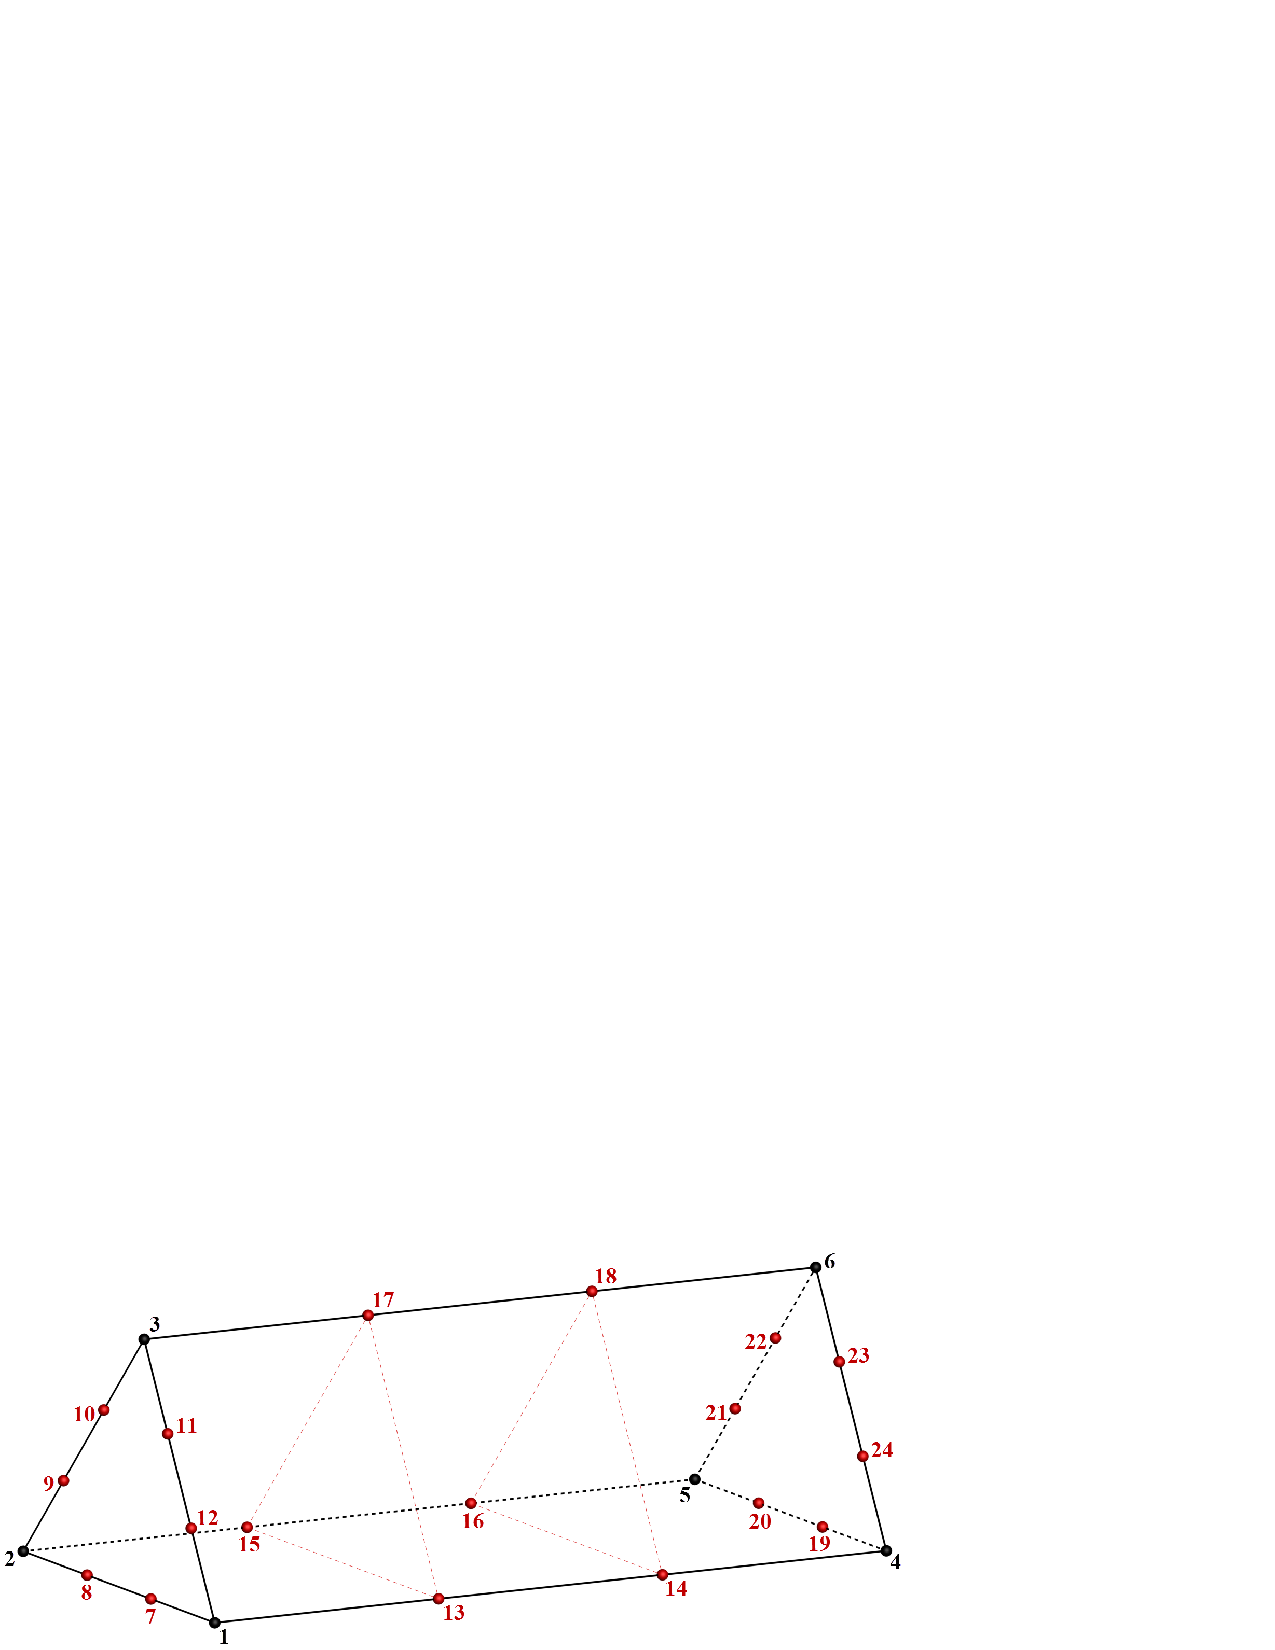
\includegraphics[width=4in]{conv.figs/TecplotFiles_Cubic_Element/All_Figures/prism_24}
\end{figure}

\bigskip

\newpage
PENTA\_38
\begin{figure}[!htb]
%   \centering
   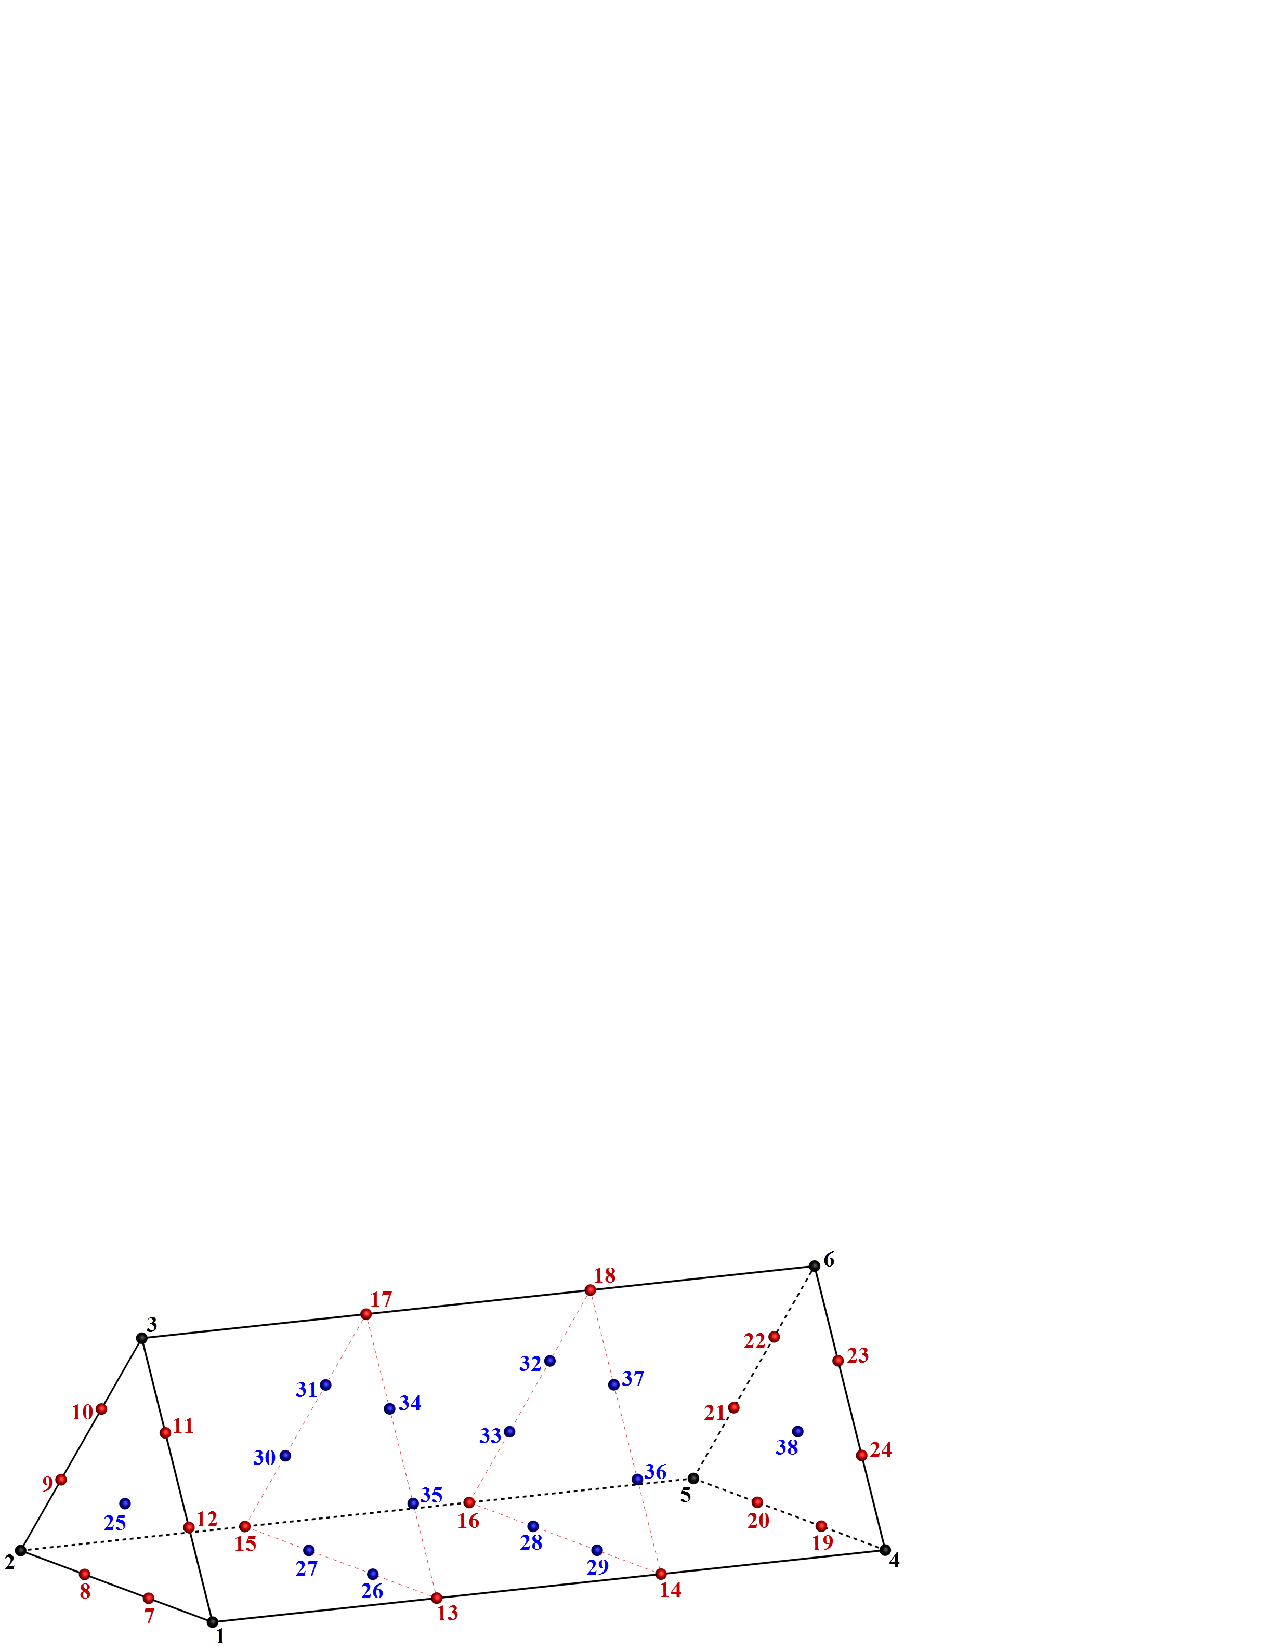
\includegraphics[width=4in]{conv.figs/TecplotFiles_Cubic_Element/All_Figures/prism_38}
\end{figure}

PENTA\_40
\begin{figure}[!htb]
%   \centering
   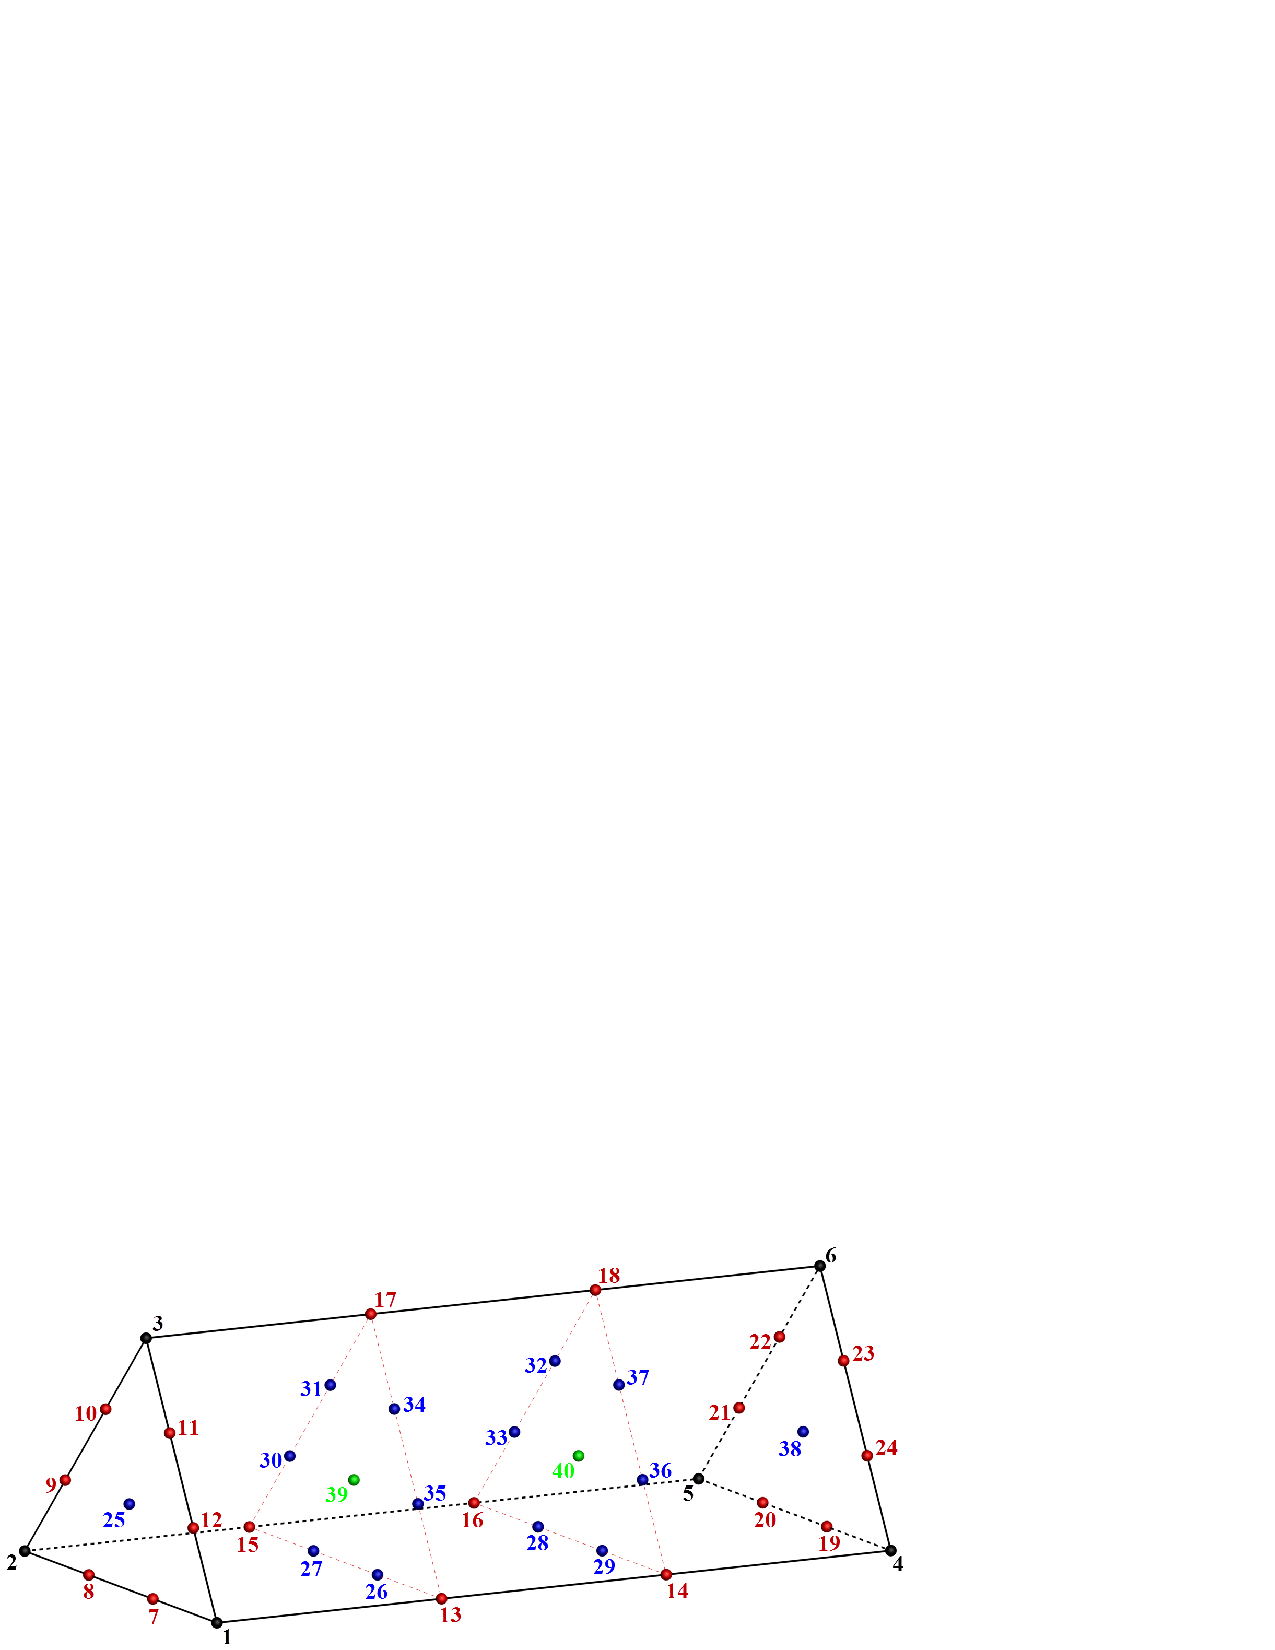
\includegraphics[width=4in]{conv.figs/TecplotFiles_Cubic_Element/All_Figures/prism_40}
\end{figure}

\begin{minipage}[t]{0.5\linewidth}
   \vspace{0pt}
   \centering
   \begin{tabular}{@{}>{\ttfamily}l >{\ttfamily}l >{\ttfamily\color{red}}l}
      \multicolumn{3}{@{}l}{\uline{\textit{Edge Definition}}} \\[6pt]
      \textnormal{Oriented}      & \textnormal{Corner}        & \textnormal{Mid-} \\
      \uline{\textnormal{edges}} & \uline{\textnormal{nodes}} & \uline{\textnormal{node}} \\[3pt]
      E1  & N1,N2 & N7,N8  \\
      E2  & N2,N3 & N9,N10  \\
      E3  & N3,N1 & N11,N12  \\
      E4  & N1,N4 & N13,N14 \\
      E5  & N2,N5 & N15,N16 \\
      E6  & N3,N6 & N17,N18 \\
      E7  & N4,N5 & N19,N20 \\
      E8  & N5,N6 & N21,N22 \\
      E9  & N6,N4 & N23,N24
   \end{tabular}
\end{minipage}

\medskip

\begin{tabular}{@{}>{\ttfamily}c >{\ttfamily}l >{\ttfamily\color{red}}l >{\ttfamily\color{blue}}c >{\ttfamily}l}
   \multicolumn{5}{@{}l}{\uline{\textit{Face Definition}}} \\[6pt]
   \uline{\textnormal{Face}} & \uline{\textnormal{Corner nodes}} & \uline{\textnormal{Mid-edge nodes}} & \uline{\textnormal{Mid-face node}} & \uline{\textnormal{Oriented edges}} \\[3pt]
   F1 & N1,N2,N5,N4 & N7,N8,N15,N16,N20,N19,N14,N13  & N26,N27,N28,N29 & \ E1,\ E5,-E7,-E4 \\
   F2 & N2,N3,N6,N5 & N9,N10,N17,N18,N22,N21,N16,N15 & N30,N31,N32,N33 & \ E2,\ E6,-E8,-E5 \\
   F3 & N3,N1,N4,N6 & N11,N12,N13,N14,N24,N23,N18,N17& N34,N35,N36,N37 & \ E3,\ E4,-E9,-E6 \\
   F4 & N1,N3,N2    & N12,N11,N10,N9,N8,N7           & N25    & -E3,-E2,-E1       \\
   F5 & N4,N5,N6    & N19,N20,N21,N22,N23,N24        & N38    & \ E7,\ E8,\ E9
\end{tabular}

\medskip

\uline{\textit{Notes}}

\begin{Ventryi}{\fort{N1,\ldots,N27}}
   \item [\fort{N1,\ldots,N40}]
         Grid point identification number.
         Integer $\ge 0$ or blank, and no two values may be the same.
         Grid points \fort{N1}\ldots\fort{N3} are in consecutive order about
         one trilateral face.
         Grid points \fort{N4}\ldots\fort{N6} are in order in the same
         direction around the opposite trilateral face.
   \item [\fort{E1,\ldots,E9}]
         Edge identification number.
         The edges are oriented from the first to the second node.
         A negative edge (e.g., \fort{-E1}) means that the edge is used in
         its reverse direction.
   \item [\fort{F1,\ldots,F5}]
         Face identification number.
         The faces are oriented so that the cross product of a vector
         from its first to second node, with a vector from its first to
         third node, is oriented outward.
\end{Ventryi}

\paragraph{Hexahedral Elements}
CGNS supports six types of hexahedral elements, \fort{HEXA\_8},
\fort{HEXA\_20}, \fort{HEXA\_27}, \fort{HEXA\_32}, \fort{HEXA\_56}, and \fort{HEXA\_64}.
\fort{HEXA\_8} elements are composed of eight nodes located at the
eight geometric corners of the hexahedron.
In addition, \fort{HEXA\_20} and \fort{HEXA\_27} elements have a node
at the middle of each of the twelve edges; \fort{HEXA\_27} adds a
node at the middle of each of the six faces, and one at the cell center.
The cubic forms of the hexahedral elements, \fort{HEXA\_32},
\fort{HEXA\_56}, and \fort{HEXA\_64}
contain two interior nodes along each edge, 24 interior face nodes
in the case of \fort{HEXA\_56} and \fort{HEXA\_64}, and an additonal
eight interior volume nodes for \fort{HEXA\_64}.

\underbar{Linear and Quadratic Elements:}

\begin{minipage}[t]{0.5\linewidth}
   \vspace{0pt}
   \centering
   \hspace*{\tmplength}\fort{HEXA\_8}\hfill\mbox{} \\[\baselineskip]
   \begin{picture}(2.0,2.0)
      \drawline(0.0,0.0)(1.5,0.0)(1.5,1.5)(0.0,1.5)(0.0,0.0)
      \drawline(1.5,0.0)(2.0,0.5)(2.0,2.0)(1.5,1.5)
      \drawline(0.0,1.5)(0.5,2.0)(2.0,2.0)
      \dashline{0.05}(0.0,0.0)(0.5,0.5)(2.0,0.5)
      \dashline{0.05}(0.5,0.5)(0.5,2.0)
      \put( 1.50, 0.00){\circle*{0.1}}
      \put( 1.55,-0.05){\makebox(0,0)[lt]{1}}
      \put( 2.00, 0.50){\circle*{0.1}}
      \put( 2.05, 0.55){\makebox(0,0)[lb]{2}}
      \put( 0.50, 0.50){\circle*{0.1}}
      \put( 0.55, 0.55){\makebox(0,0)[lb]{3}}
      \put( 0.00, 0.00){\circle*{0.1}}
      \put(-0.05,-0.05){\makebox(0,0)[rt]{4}}
      \put( 1.50, 1.50){\circle*{0.1}}
      \put( 1.45, 1.55){\makebox(0,0)[rb]{5}}
      \put( 2.00, 2.00){\circle*{0.1}}
      \put( 2.05, 2.05){\makebox(0,0)[lb]{6}}
      \put( 0.50, 2.00){\circle*{0.1}}
      \put( 0.55, 2.05){\makebox(0,0)[lb]{7}}
      \put( 0.00, 1.50){\circle*{0.1}}
      \put(-0.05, 1.55){\makebox(0,0)[rb]{8}}
   \end{picture}
\end{minipage}%
\begin{minipage}[t]{0.5\linewidth}
   \vspace{0pt}
   \centering
   \hspace*{\tmplength}\fort{HEXA\_20}\hfill\mbox{} \\[\baselineskip]
   \begin{picture}(2.0,2.0)
      \drawline(0.0,0.0)(1.5,0.0)(1.5,1.5)(0.0,1.5)(0.0,0.0)
      \drawline(1.5,0.0)(2.0,0.5)(2.0,2.0)(1.5,1.5)
      \drawline(0.0,1.5)(0.5,2.0)(2.0,2.0)
      \dashline{0.05}(0.0,0.0)(0.5,0.5)(2.0,0.5)
      \dashline{0.05}(0.5,0.5)(0.5,2.0)
      \put( 1.50, 0.00){\circle*{0.1}}
      \put( 1.55,-0.05){\makebox(0,0)[lt]{1}}
      \put( 2.00, 0.50){\circle*{0.1}}
      \put( 2.05, 0.55){\makebox(0,0)[lb]{2}}
      \put( 0.50, 0.50){\circle*{0.1}}
      \put( 0.55, 0.55){\makebox(0,0)[lb]{3}}
      \put( 0.00, 0.00){\circle*{0.1}}
      \put(-0.05,-0.05){\makebox(0,0)[rt]{4}}
      \put( 1.50, 1.50){\circle*{0.1}}
      \put( 1.45, 1.55){\makebox(0,0)[rb]{5}}
      \put( 2.00, 2.00){\circle*{0.1}}
      \put( 2.05, 2.05){\makebox(0,0)[lb]{6}}
      \put( 0.50, 2.00){\circle*{0.1}}
      \put( 0.55, 2.05){\makebox(0,0)[lb]{7}}
      \put( 0.00, 1.50){\circle*{0.1}}
      \put(-0.05, 1.55){\makebox(0,0)[rb]{8}}
      {\color{red}
       \dashline[25]{0.025}(0.25,0.25)(1.75,0.25)
       \dashline[25]{0.025}(0.75,0.00)(1.25,0.50)
       \dashline[25]{0.025}(1.50,0.75)(2.00,1.25)(0.50,1.25)(0.00,0.75)(1.50,0.75)
       \dashline[25]{0.025}(0.25,1.75)(1.75,1.75)
       \dashline[25]{0.025}(0.75,1.50)(1.25,2.00)
       \dashline[25]{0.025}(0.25,0.25)(0.25,1.75)
       \dashline[25]{0.025}(0.75,0.00)(0.75,1.50)
       \dashline[25]{0.025}(1.75,0.25)(1.75,1.75)
       \dashline[25]{0.025}(1.25,0.50)(1.25,2.00)
      }
      \put( 1.75, 0.25){\color{red}\circle*{0.1}}
      \put( 1.80, 0.20){\color{red}\makebox(0,0)[lt]{9}}
      \put( 1.25, 0.50){\color{red}\circle*{0.1}}
      \put( 1.30, 0.55){\color{red}\makebox(0,0)[lb]{10}}
      \put( 0.25, 0.25){\color{red}\circle*{0.1}}
      \put( 0.20, 0.30){\color{red}\makebox(0,0)[rb]{11}}
      \put( 0.75, 0.00){\color{red}\circle*{0.1}}
      \put( 0.70,-0.05){\color{red}\makebox(0,0)[rt]{12}}
      \put( 1.50, 0.75){\color{red}\circle*{0.1}}
      \put( 1.60, 0.75){\color{red}\makebox(0,0)[l]{13}}
      \put( 2.00, 1.25){\color{red}\circle*{0.1}}
      \put( 2.10, 1.25){\color{red}\makebox(0,0)[l]{14}}
      \put( 0.50, 1.25){\color{red}\circle*{0.1}}
      \put( 0.55, 1.30){\color{red}\makebox(0,0)[lb]{15}}
      \put( 0.00, 0.75){\color{red}\circle*{0.1}}
      \put(-0.10, 0.75){\color{red}\makebox(0,0)[r]{16}}
      \put( 1.75, 1.75){\color{red}\circle*{0.1}}
      \put( 1.80, 1.70){\color{red}\makebox(0,0)[lt]{17}}
      \put( 1.25, 2.00){\color{red}\circle*{0.1}}
      \put( 1.30, 2.05){\color{red}\makebox(0,0)[lb]{18}}
      \put( 0.25, 1.75){\color{red}\circle*{0.1}}
      \put( 0.20, 1.80){\color{red}\makebox(0,0)[rb]{19}}
      \put( 0.75, 1.50){\color{red}\circle*{0.1}}
      \put( 0.70, 1.55){\color{red}\makebox(0,0)[rb]{20}}
   \end{picture}
\end{minipage}

\vspace{1.5\baselineskip}

\begin{minipage}[t]{0.5\linewidth}
   \color{black}
   \vspace{0pt}
   \centering
   \hspace*{\tmplength}\fort{HEXA\_27}\hfill\mbox{} \\[\baselineskip]
   \begin{picture}(2.0,2.0)
      \drawline(0.0,0.0)(1.5,0.0)(1.5,1.5)(0.0,1.5)(0.0,0.0)
      \drawline(1.5,0.0)(2.0,0.5)(2.0,2.0)(1.5,1.5)
      \drawline(0.0,1.5)(0.5,2.0)(2.0,2.0)
      \dashline{0.05}(0.0,0.0)(0.5,0.5)(2.0,0.5)
      \dashline{0.05}(0.5,0.5)(0.5,2.0)
      \put( 1.50, 0.00){\circle*{0.1}}
      \put( 1.55,-0.05){\makebox(0,0)[lt]{1}}
      \put( 2.00, 0.50){\circle*{0.1}}
      \put( 2.05, 0.55){\makebox(0,0)[lb]{2}}
      \put( 0.50, 0.50){\circle*{0.1}}
      \put( 0.55, 0.55){\makebox(0,0)[lb]{3}}
      \put( 0.00, 0.00){\circle*{0.1}}
      \put(-0.05,-0.05){\makebox(0,0)[rt]{4}}
      \put( 1.50, 1.50){\circle*{0.1}}
      \put( 1.45, 1.55){\makebox(0,0)[rb]{5}}
      \put( 2.00, 2.00){\circle*{0.1}}
      \put( 2.05, 2.05){\makebox(0,0)[lb]{6}}
      \put( 0.50, 2.00){\circle*{0.1}}
      \put( 0.55, 2.05){\makebox(0,0)[lb]{7}}
      \put( 0.00, 1.50){\circle*{0.1}}
      \put(-0.05, 1.55){\makebox(0,0)[rb]{8}}
      {\color{red}
       \dashline[25]{0.025}(0.25,0.25)(1.75,0.25)
       \dashline[25]{0.025}(0.75,0.00)(1.25,0.50)
       \dashline[25]{0.025}(1.50,0.75)(2.00,1.25)(0.50,1.25)(0.00,0.75)(1.50,0.75)
       \dashline[25]{0.025}(0.25,1.75)(1.75,1.75)
       \dashline[25]{0.025}(0.75,1.50)(1.25,2.00)
       \dashline[25]{0.025}(0.25,0.25)(0.25,1.75)
       \dashline[25]{0.025}(0.75,0.00)(0.75,1.50)
       \dashline[25]{0.025}(1.75,0.25)(1.75,1.75)
       \dashline[25]{0.025}(1.25,0.50)(1.25,2.00)
      }
      \put( 1.75, 0.25){\color{red}\circle*{0.1}}
      \put( 1.80, 0.20){\color{red}\makebox(0,0)[lt]{9}}
      \put( 1.25, 0.50){\color{red}\circle*{0.1}}
      \put( 1.30, 0.55){\color{red}\makebox(0,0)[lb]{10}}
      \put( 0.25, 0.25){\color{red}\circle*{0.1}}
      \put( 0.20, 0.30){\color{red}\makebox(0,0)[rb]{11}}
      \put( 0.75, 0.00){\color{red}\circle*{0.1}}
      \put( 0.70,-0.05){\color{red}\makebox(0,0)[rt]{12}}
      \put( 1.50, 0.75){\color{red}\circle*{0.1}}
      \put( 1.60, 0.75){\color{red}\makebox(0,0)[l]{13}}
      \put( 2.00, 1.25){\color{red}\circle*{0.1}}
      \put( 2.10, 1.25){\color{red}\makebox(0,0)[l]{14}}
      \put( 0.50, 1.25){\color{red}\circle*{0.1}}
      \put( 0.55, 1.30){\color{red}\makebox(0,0)[lb]{15}}
      \put( 0.00, 0.75){\color{red}\circle*{0.1}}
      \put(-0.10, 0.75){\color{red}\makebox(0,0)[r]{16}}
      \put( 1.75, 1.75){\color{red}\circle*{0.1}}
      \put( 1.80, 1.70){\color{red}\makebox(0,0)[lt]{17}}
      \put( 1.25, 2.00){\color{red}\circle*{0.1}}
      \put( 1.30, 2.05){\color{red}\makebox(0,0)[lb]{18}}
      \put( 0.25, 1.75){\color{red}\circle*{0.1}}
      \put( 0.20, 1.80){\color{red}\makebox(0,0)[rb]{19}}
      \put( 0.75, 1.50){\color{red}\circle*{0.1}}
      \put( 0.70, 1.55){\color{red}\makebox(0,0)[rb]{20}}
      {\color{blue}
       \dashline[25]{0.025}(0.25,1.00)(1.75,1.00)
       \dashline[25]{0.025}(0.75,0.75)(1.25,1.25)
       \dashline[25]{0.025}(1.00,0.25)(1.00,1.75)
      }
      \put(1.00,0.25){\color{blue}\circle*{0.1}}
      \put(1.05,0.20){\color{blue}\makebox(0,0)[lt]{21}}
      \put(1.75,1.00){\color{blue}\circle*{0.1}}
      \put(1.80,0.95){\color{blue}\makebox(0,0)[lt]{22}}
      \put(1.25,1.25){\color{blue}\circle*{0.1}}
      \put(1.30,1.30){\color{blue}\makebox(0,0)[lb]{23}}
      \put(0.25,1.00){\color{blue}\circle*{0.1}}
      \put(0.20,1.05){\color{blue}\makebox(0,0)[rb]{24}}
      \put(0.75,0.75){\color{blue}\circle*{0.1}}
      \put(0.70,0.80){\color{blue}\makebox(0,0)[rb]{25}}
      \put(1.00,1.75){\color{blue}\circle*{0.1}}
      \put(0.95,1.80){\color{blue}\makebox(0,0)[rb]{26}}
      \put(1.00,1.00){\color{blue}\circle*{0.1}}
      \put(0.95,1.05){\color{blue}\makebox(0,0)[rb]{27}}
   \end{picture}
\end{minipage}%
\begin{minipage}[t]{0.5\linewidth}
   \vspace{0pt}
   \centering
   \begin{tabular}{@{}>{\ttfamily}l >{\ttfamily}l >{\ttfamily\color{red}}l}
      \multicolumn{3}{@{}l}{\uline{\textit{Edge Definition}}} \\[6pt]
      \textnormal{Oriented}      & \textnormal{Corner}        & \textnormal{Mid-} \\
      \uline{\textnormal{edges}} & \uline{\textnormal{nodes}} & \uline{\textnormal{node}} \\[3pt]
      E1  & N1,N2 & N9  \\
      E2  & N2,N3 & N10 \\
      E3  & N3,N4 & N11 \\
      E4  & N4,N1 & N12 \\
      E5  & N1,N5 & N13 \\
      E6  & N2,N6 & N14 \\
      E7  & N3,N7 & N15 \\
      E8  & N4,N8 & N16 \\
      E9  & N5,N6 & N17 \\
      E10 & N6,N7 & N18 \\
      E11 & N7,N8 & N19 \\
      E12 & N8,N5 & N20
   \end{tabular}
\end{minipage}

\medskip

\begin{tabular}{@{}>{\ttfamily}c >{\ttfamily}l >{\ttfamily\color{red}}l >{\ttfamily\color{blue}}c >{\ttfamily}l}
   \multicolumn{5}{@{}l}{\uline{\textit{Face Definition}}} \\[6pt]
   \uline{\textnormal{Face}} & \uline{\textnormal{Corner nodes}} & \uline{\textnormal{Mid-edge nodes}} & \uline{\textnormal{Mid-face node}} & \uline{\textnormal{Oriented edges}} \\[3pt]
   F1 & N1,N4,N3,N2 & N12,N11,N10,N9   & N21 & -E4,-E3,\ -E2,\ -E1   \\
   F2 & N1,N2,N6,N5 & N9,\ N14,N17,N13 & N22 & \ E1, E6,\ -E9,\ -E5  \\
   F3 & N2,N3,N7,N6 & N10,N15,N18,N14  & N23 & \ E2,\ E7, -E10,-E6   \\
   F4 & N3,N4,N8,N7 & N11,N16,N19,N15  & N24 & \ E3,\ E8,\ -E11,-E7  \\
   F5 & N1,N5,N8,N4 & N13,N20,N16,N12  & N25 & \ E5,-E12,-E8,\ \ E4  \\
   F6 & N5,N6,N7,N8 & N17,N18,N19,N20  & N26 & \ E9,\ E10,\ E11,\ E12
\end{tabular}

\underbar{Cubic Elements:}

HEXA\_32
\begin{figure}[!htb]
%   \centering
   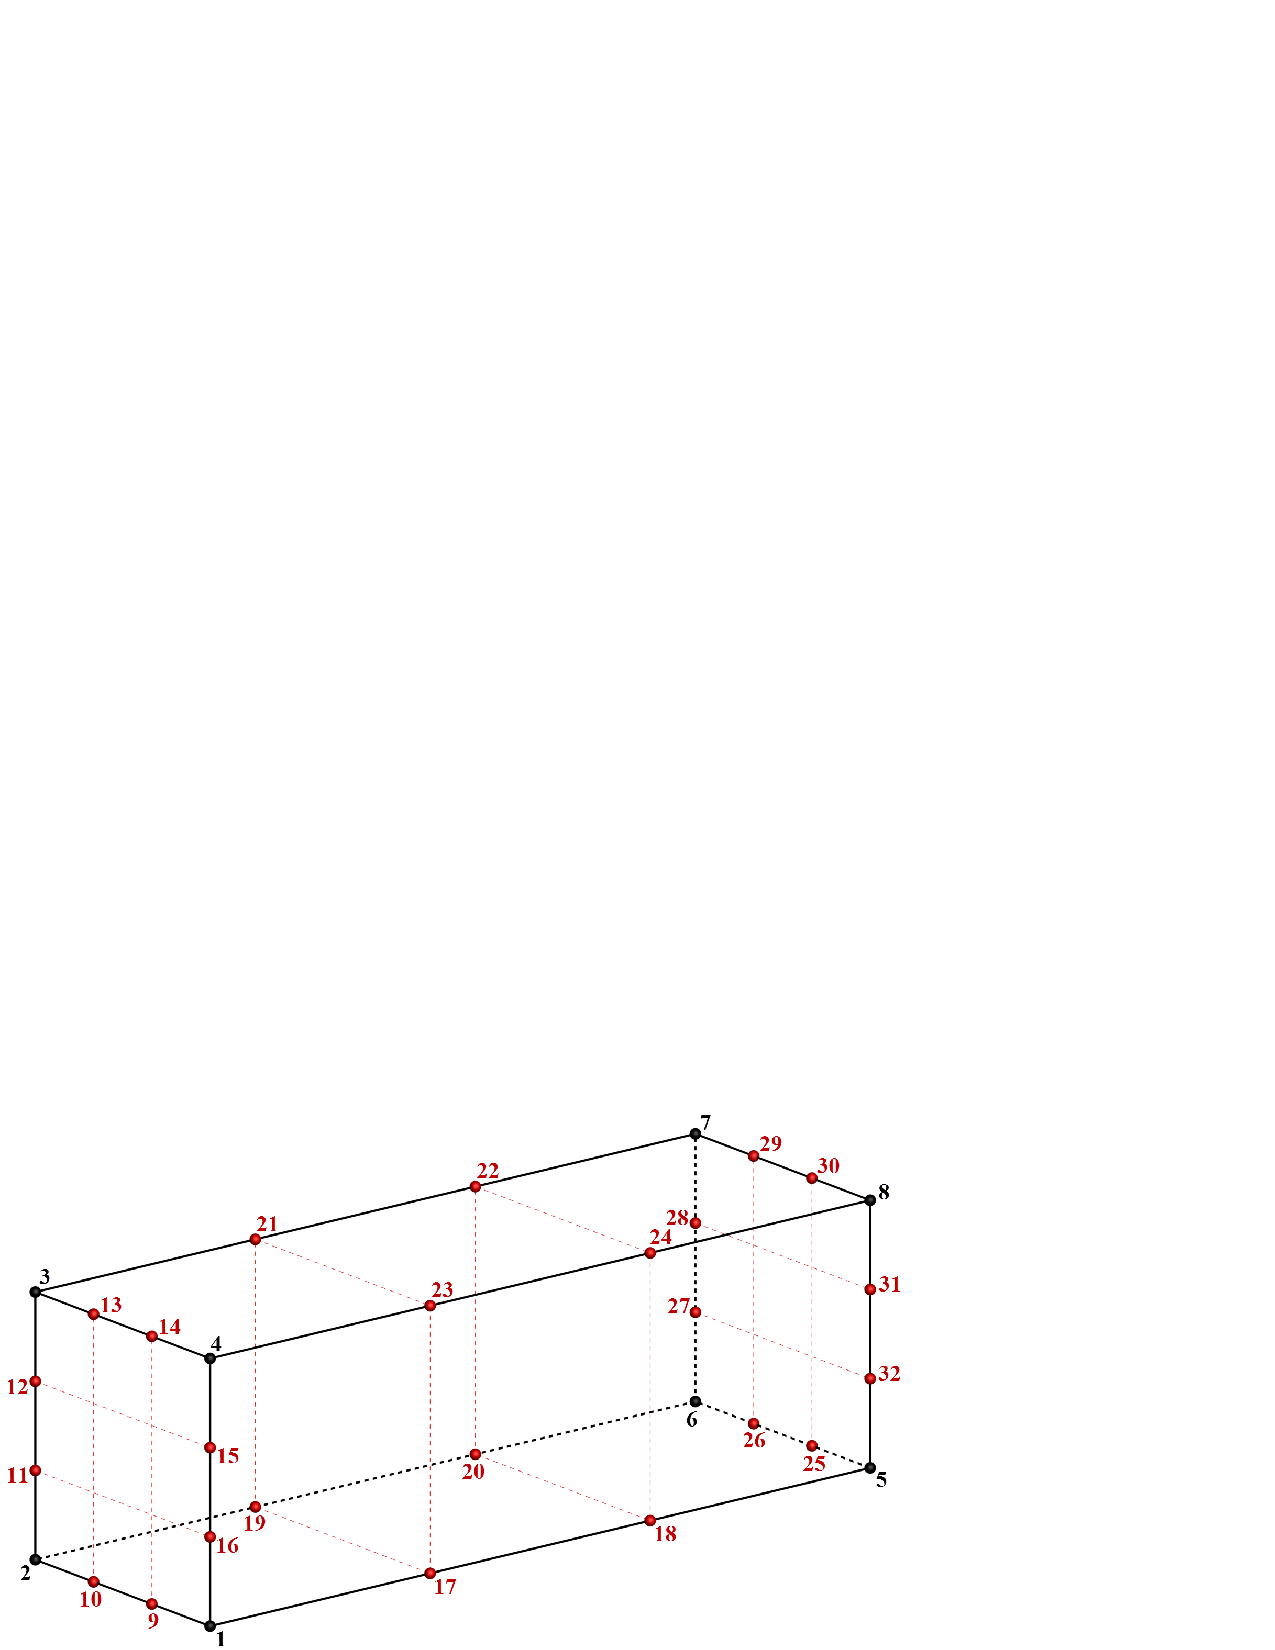
\includegraphics[width=4in]{conv.figs/TecplotFiles_Cubic_Element/All_Figures/hex_32}
\end{figure}

\bigskip

\newpage
HEXA\_56
\begin{figure}[!htb]
%   \centering
   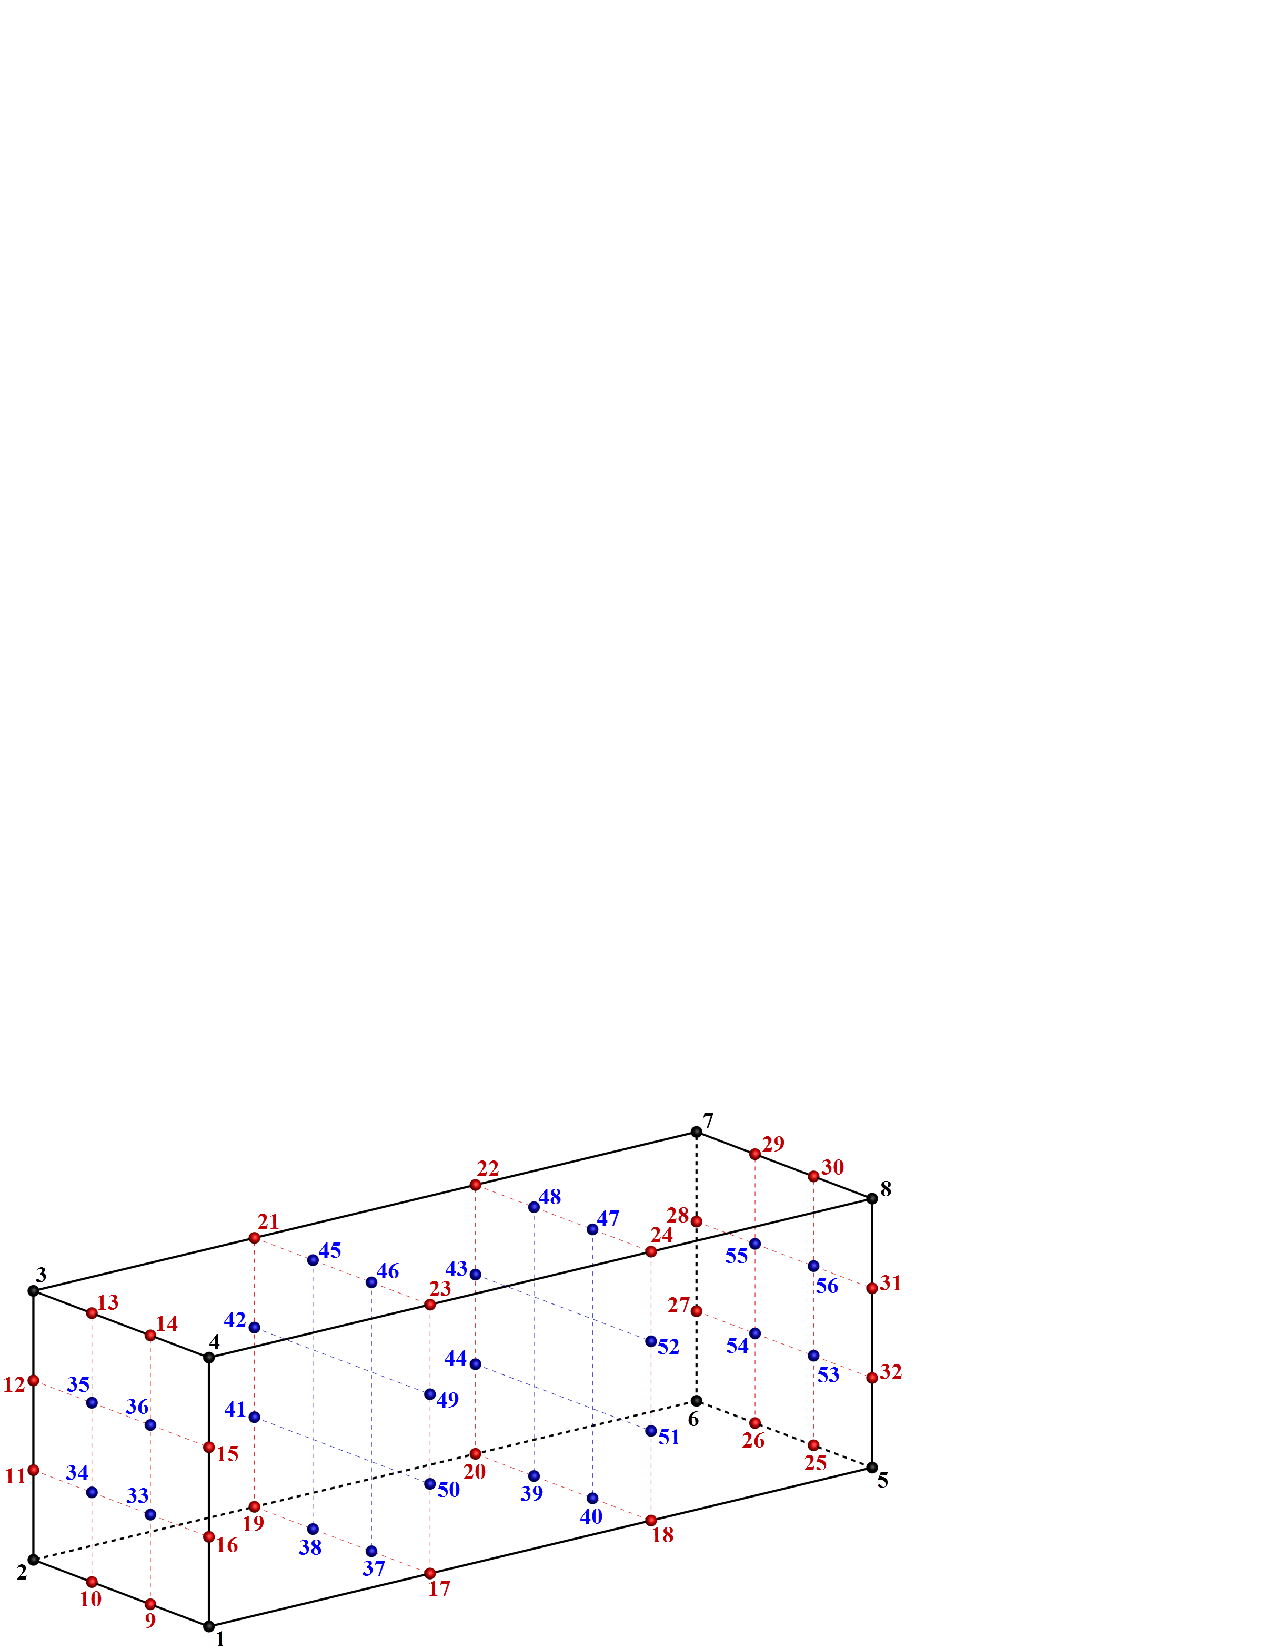
\includegraphics[width=4in]{conv.figs/TecplotFiles_Cubic_Element/All_Figures/hex_56}
\end{figure}

HEXA\_64
\begin{figure}[!htb]
%   \centering
   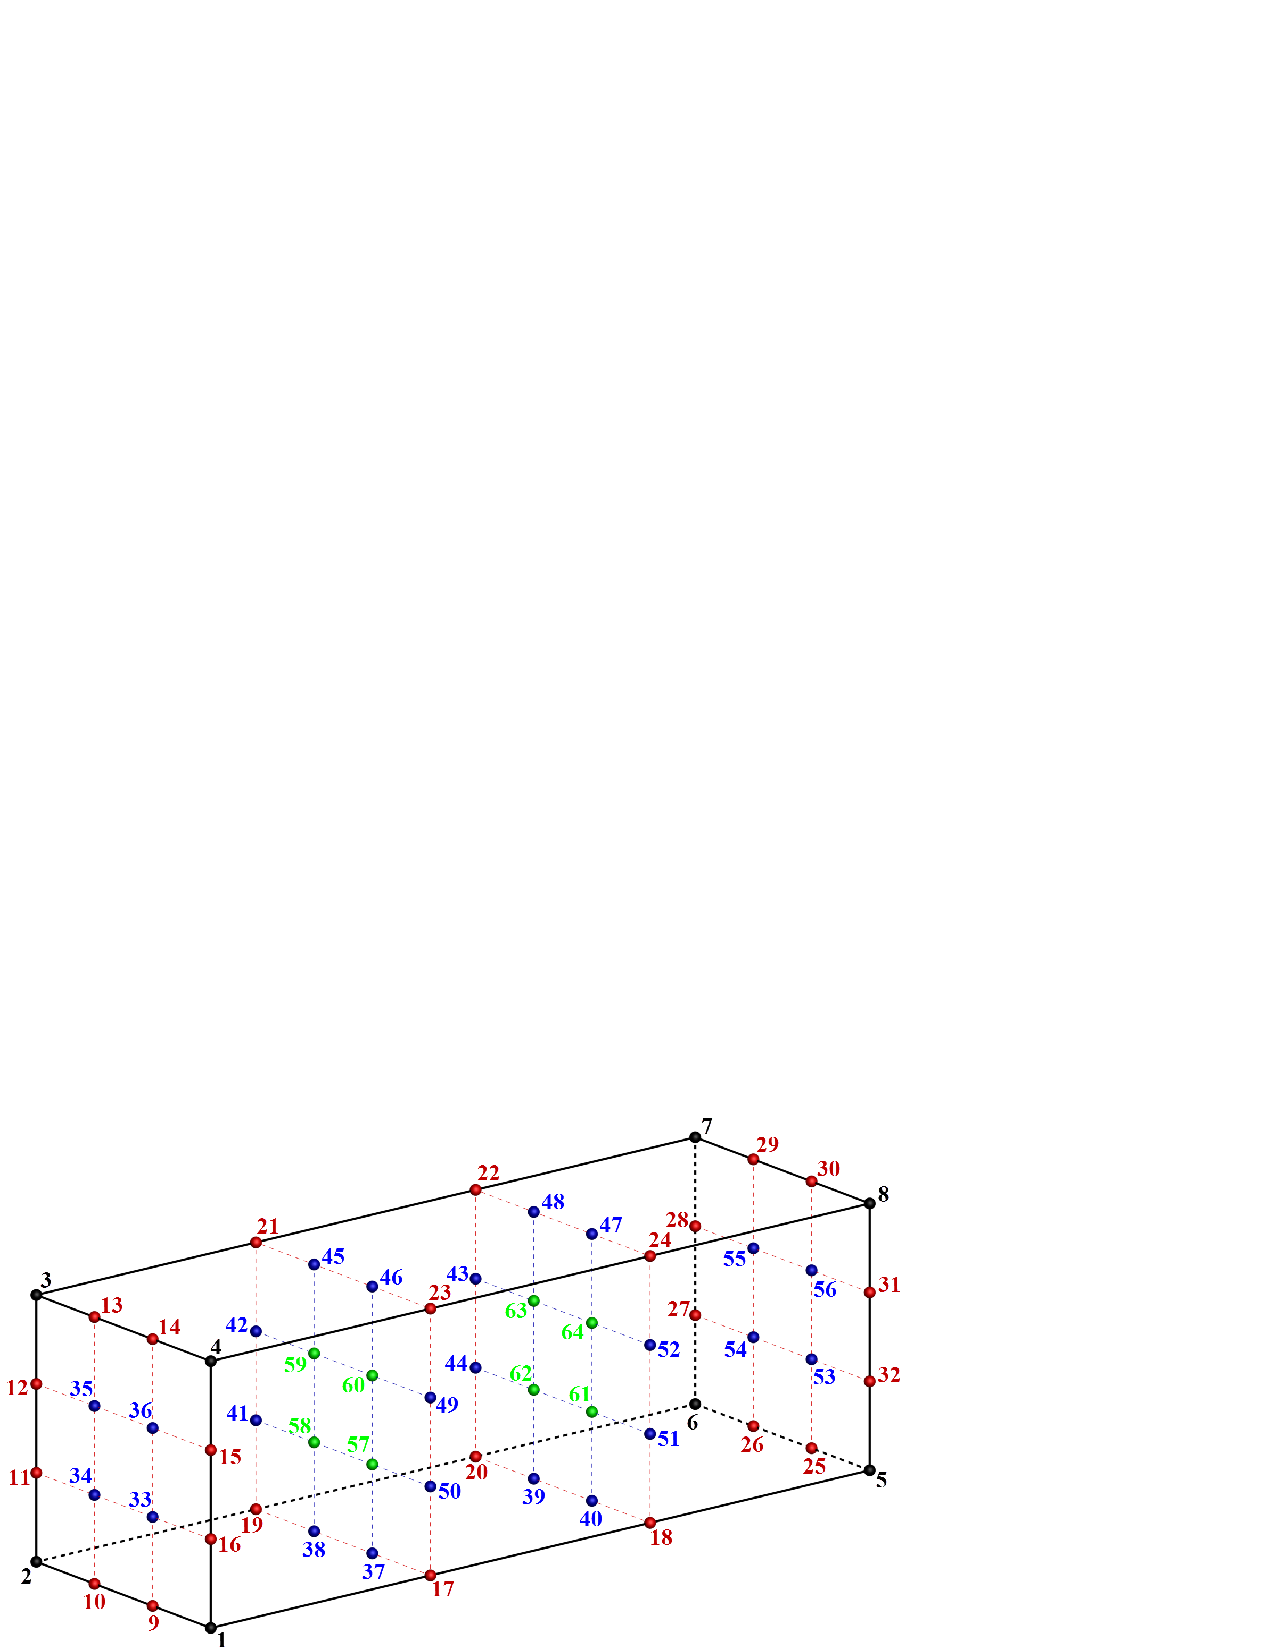
\includegraphics[width=4in]{conv.figs/TecplotFiles_Cubic_Element/All_Figures/hex_64}
\end{figure}

\begin{minipage}[t]{0.5\linewidth}
   \vspace{0pt}
   \centering
   \begin{tabular}{@{}>{\ttfamily}l >{\ttfamily}l >{\ttfamily\color{red}}l}
      \multicolumn{3}{@{}l}{\uline{\textit{Edge Definition}}} \\[6pt]
      \textnormal{Oriented}      & \textnormal{Corner}        & \textnormal{Mid-} \\
      \uline{\textnormal{edges}} & \uline{\textnormal{nodes}} & \uline{\textnormal{node}} \\[3pt]
      E1  & N1,N2 & N9,N10  \\
      E2  & N2,N3 & N11,N12 \\
      E3  & N3,N4 & N13,N14 \\
      E4  & N4,N1 & N15,N16 \\
      E5  & N1,N5 & N17,N18 \\
      E6  & N2,N6 & N19,N20 \\
      E7  & N3,N7 & N21,N22 \\
      E8  & N4,N8 & N23,N24 \\
      E9  & N5,N6 & N25,N26 \\
      E10 & N6,N7 & N27,N28 \\
      E11 & N7,N8 & N29,N30 \\
      E12 & N8,N5 & N31,N32
   \end{tabular}
\end{minipage}

\medskip

\begin{tabular}{@{}>{\ttfamily}c >{\ttfamily}l >{\ttfamily\color{red}}l >{\ttfamily\color{blue}}c >{\ttfamily}l}
   \multicolumn{5}{@{}l}{\uline{\textit{Face Definition}}} \\[6pt]
   \uline{\textnormal{Face}} & \uline{\textnormal{Corner nodes}} & \uline{\textnormal{Mid-edge nodes}} & \uline{\textnormal{Mid-face node}} & \uline{\textnormal{Oriented edges}} \\[3pt]
   F1 & N1,N4,N3,N2 & N16,N15,N14,N13,N12,N11,N10,N9   & N33,N36,N35,N34 & -E4,-E3,\ -E2,\ -E1   \\
   F2 & N1,N2,N6,N5 & N9,N10,N19,N20,N26,N25,N18,N17   & N37,N38,N39,N40 & \ E1, E6,\ -E9,\ -E5  \\
   F3 & N2,N3,N7,N6 & N11,N12,N21,N22,N28,N27,N20,N19  & N41,N42,N43,N44 & \ E2,\ E7, -E10,-E6   \\
   F4 & N3,N4,N8,N7 & N13,N14,N23,N24,N30,N29,N22,N21  & N45,N46,N47,N48 & \ E3,\ E8,\ -E11,-E7  \\
   F5 & N1,N5,N8,N4 & N17,N18,N32,N31,N24,N23,N15,N16  & N49,N50,N51,N52 & \ E5,-E12,-E8,\ \ E4  \\
   F6 & N5,N6,N7,N8 & N25,N26,N27,N28,N29,N30,N31,N32  & N53,N54,N55,N56 & \ E9,\ E10,\ E11,\ E12
\end{tabular}

\medskip

\uline{\textit{Notes}}

\begin{Ventryi}{\fort{N1,\ldots,N27}}
   \item [\fort{N1,\ldots,N64}]
         Grid point identification number.
         Integer $\ge 0$ or blank, and no two values may be the same.
         Grid points \fort{N1}\ldots\fort{N4} are in consecutive order about
         one quadrilateral face.
         Grid points \fort{N5}\ldots\fort{N8} are in order in the same
         direction around the opposite quadrilateral face.
   \item [\fort{E1,\ldots,E12}]
         Edge identification number.
         The edges are oriented from the first to the second node.
         A negative edge (e.g., \fort{-E1}) means that the edge is used in
         its reverse direction.
   \item [\fort{F1,\ldots,F6}]
         Face identification number.
         The faces are oriented so that the cross product of a vector
         from its first to second node, with a vector from its first to
         third node, is oriented outward.
\end{Ventryi}

\subsubsection{Unstructured Grid Example}
\label{s:unst_example}

Consider an unstructured zone in the shape of a cube, with each edge
of the zone having three nodes.
The resulting unstructured grid has a total of 27 nodes, as illustrated
in the exploded figure below.

\begin{center}
   \begin{picture}(4.0,4.0)(-1.0,-1.0)
%     Zone outline
      \drawline(0.0,0.0)(1.5,0.0)(1.5,1.5)(0.0,1.5)(0.0,0.0)
      \drawline(1.5,0.0)(2.0,0.5)(2.0,2.0)(1.5,1.5)
      \drawline(0.0,1.5)(0.5,2.0)(2.0,2.0)
      \dashline{0.05}(0.0,0.0)(0.5,0.5)(2.0,0.5)
      \dashline{0.05}(0.5,0.5)(0.5,2.0)
%     Remaining cell boundaries
      \drawline(0.0,0.75)(1.5,0.75)
      \drawline(0.75,0.0)(0.75,1.5)
      \drawline(1.5,0.75)(2.0,1.25)
      \drawline(1.75,0.25)(1.75,1.75)
      \drawline(0.25,1.75)(1.75,1.75)
      \drawline(0.75,1.5)(1.25,2.0)
      \dashline{0.05}(0.25,0.25)(1.75,0.25)
      \dashline{0.05}(0.75,0.0)(1.25,0.5)
      \dashline{0.05}(0.0,0.75)(0.5,1.25)
      \dashline{0.05}(0.25,0.25)(0.25,1.75)
      \dashline{0.05}(0.5,1.25)(2.0,1.25)
      \dashline{0.05}(1.25,0.5)(1.25,2.0)
      \dashline{0.05}(0.25,1.0)(1.75,1.0)
      \dashline{0.05}(0.75,0.75)(1.25,1.25)
%     Bottom nodes
      \put( 0.00, 0.00){\circle*{0.05}}
      \put(-0.05,-0.05){\makebox(0,0)[rt]{19}}
      \put( 0.75, 0.00){\circle*{0.05}}
      \put( 1.50, 0.00){\circle*{0.05}}
      \put( 1.55,-0.05){\makebox(0,0)[lt]{21}}
      \put( 0.25, 0.25){\circle*{0.05}}
      \put( 1.00, 0.25){\circle*{0.05}}
      \put( 1.75, 0.25){\circle*{0.05}}
      \put( 0.50, 0.50){\circle*{0.05}}
      \put( 0.55, 0.45){\makebox(0,0)[lt]{1}}
      \put( 1.25, 0.50){\circle*{0.05}}
      \put( 2.00, 0.50){\circle*{0.05}}
      \put( 2.05, 0.45){\makebox(0,0)[lt]{3}}
%     Middle nodes
      \put( 0.00, 0.75){\circle*{0.05}}
      \put( 0.75, 0.75){\circle*{0.05}}
      \put( 0.70, 0.70){\makebox(0,0)[rt]{23}}
      \put( 1.50, 0.75){\circle*{0.05}}
      \put( 0.25, 1.00){\circle*{0.05}}
      \put( 1.00, 1.00){\circle*{0.05}}
      \put( 1.05, 0.95){\makebox(0,0)[lt]{14}}
      \put( 1.75, 1.00){\circle*{0.05}}
      \put( 0.50, 1.25){\circle*{0.05}}
      \put( 1.25, 1.25){\circle*{0.05}}
      \put( 1.30, 1.20){\makebox(0,0)[lt]{5}}
      \put( 2.00, 1.25){\circle*{0.05}}
%     Top nodes
      \put( 0.00, 1.50){\circle*{0.05}}
      \put(-0.05, 1.55){\makebox(0,0)[rb]{25}}
      \put( 0.75, 1.50){\circle*{0.05}}
      \put( 1.50, 1.50){\circle*{0.05}}
      \put( 1.45, 1.55){\makebox(0,0)[rb]{27}}
      \put( 0.25, 1.75){\circle*{0.05}}
      \put( 1.00, 1.75){\circle*{0.05}}
      \put( 1.75, 1.75){\circle*{0.05}}
      \put( 0.50, 2.00){\circle*{0.05}}
      \put( 0.55, 2.05){\makebox(0,0)[lb]{7}}
      \put( 1.25, 2.00){\circle*{0.05}}
      \put( 2.00, 2.00){\circle*{0.05}}
      \put( 2.05, 2.05){\makebox(0,0)[lb]{9}}
%     Bottom exploded face
      \drawline(0.0,-1.0)(1.5,-1.0)(2.0,-0.5)
      \dashline{0.05}(0.0,-1.0)(0.5,-0.5)(2.0,-0.5)
      \dashline{0.05}(0.25,-0.75)(1.75,-0.75)
      \dashline{0.05}(0.75,-1.0)(1.25,-0.5)
      \put( 0.00,-1.00){\circle*{0.05}}
      \put(-0.05,-1.05){\makebox(0,0)[rt]{19}}
      \put( 0.75,-1.00){\circle*{0.05}}
      \put( 0.70,-1.05){\makebox(0,0)[rt]{20}}
      \put( 1.50,-1.00){\circle*{0.05}}
      \put( 1.55,-1.05){\makebox(0,0)[lt]{21}}
      \put( 0.25,-0.75){\circle*{0.05}}
      \put( 0.20,-0.70){\makebox(0,0)[rb]{10}}
      \put( 1.00,-0.75){\circle*{0.05}}
      \put( 0.95,-0.70){\makebox(0,0)[rb]{11}}
      \put( 1.75,-0.75){\circle*{0.05}}
      \put( 1.80,-0.80){\makebox(0,0)[lt]{12}}
      \put( 0.50,-0.50){\circle*{0.05}}
      \put( 0.45,-0.45){\makebox(0,0)[rb]{1}}
      \put( 1.25,-0.50){\circle*{0.05}}
      \put( 1.30,-0.45){\makebox(0,0)[lb]{2}}
      \put( 2.00,-0.50){\circle*{0.05}}
      \put( 2.05,-0.45){\makebox(0,0)[lb]{3}}
%     Top exploded face
      \drawline(0.0,2.5)(1.5,2.5)(2.0,3.0)
      \drawline(0.0,2.5)(0.5,3.0)(2.0,3.0)
      \drawline(0.25,2.75)(1.75,2.75)
      \drawline(0.75,2.5)(1.25,3.0)
      \put( 0.00, 2.50){\circle*{0.05}}
      \put(-0.05, 2.45){\makebox(0,0)[rt]{25}}
      \put( 0.75, 2.50){\circle*{0.05}}
      \put( 0.70, 2.45){\makebox(0,0)[rt]{26}}
      \put( 1.50, 2.50){\circle*{0.05}}
      \put( 1.55, 2.45){\makebox(0,0)[lt]{27}}
      \put( 0.25, 2.75){\circle*{0.05}}
      \put( 0.20, 2.80){\makebox(0,0)[rb]{16}}
      \put( 1.00, 2.75){\circle*{0.05}}
      \put( 0.95, 2.80){\makebox(0,0)[rb]{17}}
      \put( 1.75, 2.75){\circle*{0.05}}
      \put( 1.80, 2.70){\makebox(0,0)[lt]{18}}
      \put( 0.50, 3.00){\circle*{0.05}}
      \put( 0.45, 3.05){\makebox(0,0)[rb]{7}}
      \put( 1.25, 3.00){\circle*{0.05}}
      \put( 1.30, 3.05){\makebox(0,0)[lb]{8}}
      \put( 2.00, 3.00){\circle*{0.05}}
      \put( 2.05, 3.05){\makebox(0,0)[lb]{9}}
%     Left exploded face
      \drawline(-1.0,0.0)(-1.0,1.5)(-0.5,2.0)
      \dashline{0.05}(-1.0,0.0)(-0.5,0.5)(-0.5,2.0)
      \dashline{0.05}(-1.0,0.75)(-0.5,1.25)
      \dashline{0.05}(-0.75,0.25)(-0.75,1.75)
      \put(-1.00, 0.00){\circle*{0.05}}
      \put(-1.05,-0.05){\makebox(0,0)[rt]{19}}
      \put(-1.00, 0.75){\circle*{0.05}}
      \put(-1.05, 0.70){\makebox(0,0)[rt]{22}}
      \put(-1.00, 1.25){\circle*{0.05}}
      \put(-1.05, 1.30){\makebox(0,0)[rb]{25}}
      \put(-0.75, 0.25){\circle*{0.05}}
      \put(-0.70, 0.20){\makebox(0,0)[lt]{10}}
      \put(-0.75, 1.00){\circle*{0.05}}
      \put(-0.70, 0.95){\makebox(0,0)[lt]{13}}
      \put(-0.75, 1.75){\circle*{0.05}}
      \put(-0.80, 1.80){\makebox(0,0)[rb]{16}}
      \put(-0.50, 0.50){\circle*{0.05}}
      \put(-0.45, 0.45){\makebox(0,0)[lt]{1}}
      \put(-0.50, 1.25){\circle*{0.05}}
      \put(-0.45, 1.30){\makebox(0,0)[lb]{4}}
      \put(-0.50, 2.00){\circle*{0.05}}
      \put(-0.45, 2.05){\makebox(0,0)[lb]{7}}
%     Right exploded face
      \drawline(2.5,0.0)(2.5,1.5)(3.0,2.0)
      \drawline(2.5,0.0)(3.0,0.5)(3.0,2.0)
      \drawline(2.5,0.75)(3.0,1.25)
      \drawline(2.75,0.25)(2.75,1.75)
      \put( 2.50, 0.00){\circle*{0.05}}
      \put( 2.45,-0.05){\makebox(0,0)[rt]{21}}
      \put( 2.50, 0.75){\circle*{0.05}}
      \put( 2.45, 0.70){\makebox(0,0)[rt]{24}}
      \put( 2.50, 1.25){\circle*{0.05}}
      \put( 2.45, 1.30){\makebox(0,0)[rb]{27}}
      \put( 2.75, 0.25){\circle*{0.05}}
      \put( 2.80, 0.20){\makebox(0,0)[lt]{12}}
      \put( 2.75, 1.00){\circle*{0.05}}
      \put( 2.80, 0.95){\makebox(0,0)[lt]{15}}
      \put( 2.75, 1.75){\circle*{0.05}}
      \put( 2.70, 1.80){\makebox(0,0)[rb]{18}}
      \put( 3.00, 0.50){\circle*{0.05}}
      \put( 3.05, 0.45){\makebox(0,0)[lt]{3}}
      \put( 3.00, 1.25){\circle*{0.05}}
      \put( 3.05, 1.30){\makebox(0,0)[lb]{6}}
      \put( 3.00, 2.00){\circle*{0.05}}
      \put( 3.05, 2.05){\makebox(0,0)[lb]{9}}
   \end{picture}
\end{center}

This zone contains eight hexahedral cells, numbered 1 to 8, and the
cell connectivity is:

\begin{center}
\begin{tabular}{c >{\quad}l}
\hline\hline \\*[-2ex]
\bold{Element No.} & \bold{Element Connectivity}
\\*[1ex] \hline\hline \\*[-2ex]
1 & \phantom{0}1, \phantom{0}2, \phantom{0}5, \phantom{0}4, 10, 11, 14, 13 \\
2 & \phantom{0}2, \phantom{0}3, \phantom{0}6, \phantom{0}5, 11, 12, 15, 14 \\
3 & \phantom{0}4, \phantom{0}5, \phantom{0}8, \phantom{0}7, 13, 14, 17, 16 \\
4 & \phantom{0}5, \phantom{0}6, \phantom{0}9, \phantom{0}8, 14, 15, 18, 17 \\
5 & 10, 11, 14, 13, 19, 20, 23, 22 \\
6 & 11, 12, 15, 14, 20, 21, 24, 23 \\
7 & 13, 14, 17, 16, 22, 23, 26, 25 \\
8 & 14, 15, 18, 17, 23, 24, 27, 26
\\*[1ex] \hline\hline
\end{tabular}
\end{center}

In addition to the cells, the boundary faces could also be added to the
element definition of this unstructured zone.
There are 24 boundary faces in this zone, corresponding to element
numbers 9 to 32.
Each boundary face is of type \fort{QUAD\_4}.
The table below shows the element connectivity of each boundary face,
as well as the element number and face number of its parent cell.

\begin{center}
\begin{tabular}{l >{\quad}c >{\quad}c >{\quad}c >{\quad}c}
\\ \hline\hline \\*[-2ex]
                      &                              & \bold{Element}      & \bold{Parent} & \bold{Parent} \\
\spantwo{\bold{Face}} & \spantwo{\bold{Element No.}} & \bold{Connectivity} & \bold{Cell}   & \bold{Face}
\\*[1ex] \hline\hline \\*[-2ex]
Left   & \phantom{0}9 & \phantom{0}1, 10, 13, \phantom{0}4 & 1 & 5 \\
       &           10 & \phantom{0}4, 13, 16, \phantom{0}7 & 3 & 5 \\
       &           11 &           10, 19, 22,           13 & 5 & 5 \\
       &           12 &           13, 22, 25,           16 & 7 & 5 \\
\\
Right  & 13 & \phantom{0}3, \phantom{0}6, 15, 12 & 2 & 3 \\
       & 14 & \phantom{0}6, \phantom{0}9, 18, 15 & 4 & 3 \\
       & 15 &           12,           15, 24, 21 & 6 & 3 \\
       & 16 &           15,           18, 27, 24 & 8 & 3 \\
\\
Bottom & 17 & \phantom{0}1, \phantom{0}2, 11, 10 & 1 & 2 \\
       & 18 & \phantom{0}2, \phantom{0}3, 12, 11 & 2 & 2 \\
       & 19 &           10,           11, 20, 19 & 5 & 2 \\
       & 20 &           11,           12, 21, 20 & 6 & 2 \\
\\
Top    & 21 & \phantom{0}7, 16, 17, \phantom{0}8 & 3 & 4 \\
       & 22 & \phantom{0}8, 17, 18, \phantom{0}9 & 4 & 4 \\
       & 23 &           16, 25, 26,           17 & 7 & 4 \\
       & 24 &           17, 26, 27,           18 & 8 & 4 \\
\\
Back   & 25 & \phantom{0}1, \phantom{0}4, \phantom{0}5, \phantom{0}2 & 1 & 1 \\
       & 26 & \phantom{0}2, \phantom{0}5, \phantom{0}6, \phantom{0}3 & 2 & 1 \\
       & 27 & \phantom{0}4, \phantom{0}7, \phantom{0}8, \phantom{0}5 & 3 & 1 \\
       & 28 & \phantom{0}5, \phantom{0}8, \phantom{0}9, \phantom{0}6 & 4 & 1 \\
\\
Front  & 29 & 19, 20, 23, 22 & 5 & 6 \\
       & 30 & 20, 21, 24, 23 & 6 & 6 \\
       & 31 & 22, 23, 26, 25 & 7 & 6 \\
       & 32 & 23, 24, 27, 26 & 8 & 6 
\\*[1ex] \hline\hline
\end{tabular}
\end{center}
%\end{longtable}

\subsection{Multizone Interfaces}
\label{s:interface_types}

% interface.tex	 multizone interface types figure

\begin{figure}[htp]
\begin{picture}(6.5,6.0)
% \put(0,0){\framebox(6.5,6.0){}}

 %  1-to-1 interface
 \put(0,4.7){%
 \begin{picture}(0,0)
  \multiput(0,0)(0,0.3){ 6}{\line(1,0){2.0}}
  \multiput(0,0)(0.2,0){11}{\line(0,1){1.5}}
  \multiput(2.0,0)(0,0.3){5}{\circle*{0.04}}
  
  \multiput(2.0,0)(0,0.3){5}{\line(1,0){1.5}}
  \multiput(2.0,0)(0.3,0){6}{\line(0,1){1.2}}
  
  \put(3.7,1.0){\makebox(0,0)[lt]{%
   \begin{tabular}{c@{\quad}p{3.25in}}
    $\bullet$ & Left-zone vertices on interface
   \end{tabular}}}
 \end{picture}}
 
 \put(0,4.5){\makebox(6,0){(a) 1-to-1 Abutting Interface}}

 %  mismatch interface
 \put(0,2.7){%
 \begin{picture}(0,0)
  \multiput(0,0)(0,0.3){ 6}{\line(1,0){2.0}}
  \multiput(0,0)(0.2,0){11}{\line(0,1){1.5}}
  \multiput(2.0,0.3)(0,0.3){4}{\circle*{0.04}}
  \multiput(2.0,0.45)(0,0.3){4}{\makebox(0,0){$\times$}}
  
  \multiput(2.0,0.22)(0,0.2){7}{\line(1,0){1.5}}
  \multiput(2.0,0.22)(0.3,0){6}{\line(0,1){1.2}}
  
  \put(3.7,1.0){\makebox(0,0)[lt]{%
   \begin{tabular}{c@{\quad}p{3.25in}}
    $\bullet$ & Left-zone vertices on interface \\
    $\times$  & Left-zone face-centers on interface
   \end{tabular}}}
 \end{picture}}
 
 \put(0,2.5){\makebox(6,0){(b) Mismatched Abutting Interface}}

 %  overset interface
 \put(0,0.3){%
 \begin{picture}(0,0)
  \multiput(0,0)(0,0.3){ 6}{\line(1,0){2.0}}
  \multiput(0,0)(0.2,0){11}{\line(0,1){1.5}}
 
  \put(1.8,0  ){\circle*{0.04}}
  \put(1.6,0.3){\circle*{0.04}}
  \put(1.4,0.6){\circle*{0.04}}
  \put(1.2,0.9){\circle*{0.04}}
  \put(1.4,1.2){\circle*{0.04}}
  \put(1.6,1.2){\circle*{0.04}}
  \put(1.8,1.5){\circle*{0.04}}
  
  \multiput(2.0,0.0)(0,0.3){6}{\circle{0.06}}
  \multiput(1.8,0.3)(0,0.3){4}{\circle{0.06}}
  \put(1.6,0.6){\circle{0.06}}
  \put(1.6,0.9){\circle{0.06}}
  \put(1.4,0.9){\circle{0.06}}
  
  \multiput(1.8,-0.2)(-0.1,0.15){9}{\line(3,2){1.5}}
  \multiput(1.8,-0.2)(0.3,0.2){6}{\line(-2,3){0.8}}
  
  \put(3.7,1.0){\makebox(0,0)[lt]{%
   \begin{tabular}{c@{\quad}p{3.25in}}
    $\bullet$ & Left-zone fringe points (vertices) \\
    $\circ$   & Left-zone overset-hole points (vertices)
   \end{tabular}}}
 \end{picture}}
 
 \put(0,0){\makebox(6,0){(c) Overset Interface}}

\end{picture}
\caption{Structured-Grid Multizone Interface Types}
\label{f:interface}
\end{figure}


\autoref{f:interface} depicts three types of multizone interfaces, shown
for structured zones.
The first type is a 1-to-1 abutting interface, also referred to as
matching or C0 continuous.
The interface is a plane of vertices that are physically coincident
between the adjacent zones.
For structured zones, grid-coordinate lines perpendicular to
the interface are continuous from one zone to the next;
in 3-D, a 1-to-1 abutting interface is usually a logically rectangular
region.

The second type of interface is mismatched abutting, where two zones
touch but do not overlap (except for vertices and cell faces on the grid
plane of the interface).
Vertices on the interface may not be physically coincident between the two
zones.
\autoref{f:interface}b identifies the vertices and face centers
of the left zone that lay on the interface.
Even for structured zones in 3-D, the vertices of a zone that constitute
an interface patch may not form a logically rectangular region.

The third type of multizone interface is called overset and occurs when
two zones overlap; in 3-D, the overlap is a 3-D region.
For overset interfaces, one of the two zones takes precedence over the
other; this establishes which solution in the overlap region to retain
and which to discard.
The region in a given zone where the solution is discarded is called an
overset hole and the grid points outlining the hole are called fringe
points.
\autoref{f:interface}c depicts an overlap region between two zones.
The right zone takes precedence over the left zone, and the points
identified in the figure are the fringe points and overset-hole points
for the left zone.
In addition, for the zone taking precedence, any bounding points
(i.e., vertices on the bounding faces) of the zone that lay within the
overlap region must also be identified.

Overset interfaces may also include multiple layers of fringe points
outlining holes and at zone boundaries.

For the mismatched abutting and overset interfaces in
\autoref{f:interface}, the left zone plays the role of receiver zone and
the right plays the role of donor zone.
